\clearpage

\section {Updated results with $E_b$ parameter and \dmsq smearing}
\label{sec:results2017b}

\subsection{Findings from the 2017 fake data studies}

As part of the analysis procedure, a variety of fake data fits were performed to assess the robustness of the analysis to changes in the cross-section model \cite{FakeData:2017}. The conclusion of these fake data studies was that an additional source of uncertainty was necessary to address biases seen in \ssqthtwothree and \dmsq (\dmsqtwothree for normal hierarchy or \dmsqonethree for inverted hierarchy) in the $E_b$ fake data studies. Furthermore, the inclusion of the additional systematic parameter was insufficient to address the bias in \dmsq and therefore an additional smearing of the likelihood surface for this parameter was added.

\subsection{Systematic parameter update and smearing procedure}

The additional $E_b$ systematic parameter is implemented as a response function, based on weights determined by the ratio of near-to-far predicted fake data event rates and event rates seen in the fake data set. The ratio was calculated for 3 points; $-0.5\sigma$, $0\sigma$ and $+1\sigma$, with  a further 3 linearly extrapolated points at $-1.5\sigma$, $+3\sigma$ and $+5\sigma$ included to allow the response function to better conform to bi-linearity throughout the allowed $[-1.5\sigma, +5\sigma]$ range. \color{blue}Negative weights that can result from the extrapolation are set to zero.\color{black}

Post-fit, the \dmsq contour is inflated via a smearing procedure. In particular, the likelihood surface resulting from the fit is scaled by a factor of 10 and resampled using Catmull-Rom cubic interpolation, before each source bin in \dmsq (for a particular value of \ssqthtwothree in the 2D fit) is smeared over the remaining \dmsq bins, with the contribution weighted by a Gaussian centred on the source bin, integrated over the target bin interval.

\subsection{Results}

The results of the \RunPeriod data set fit, for an exposure of \TotalPotNuRunOneEight POT in neutrino mode and of \TotalPotNuBarRunOneEight POT in antineutrino mode, with the $E_b$ parameter and smearing applied, are shown in this chapter.  In \cref{fig:asimovpf_spectra_mc_data_2017b} the best-fit predicted spectra of $\mu$-like and $e$-like samples are compared to the observed data. In \cref{tab:num_events_run18_2017b} the expected and observed number of events in \RunPeriod data set are shown.

\begin{table}[htb]
\centering
\begin{tabular}{| c | c | c | c |}
\hline
Beam mode & Sample & Exp. Best-fit & Observed \\
\hline
$\nu$ & $\mu$-like & 270.792 & 240 \\
$\nu$ & $e$-like & 73.099 & 74 \\
$\bar{\nu}$ & $\mu$-like & 64.997 & 68 \\
$\bar{\nu}$ & $e$-like & 7.947 & 7 \\
$\nu$ & \nueCConepi-like & 6.812 & 15 \\
\hline
\end{tabular}

\caption{
The observed and best-fit expected number of events in \RunPeriod data set for an exposure of \TotalPotNuRunOneEight POT in neutrino mode and of \TotalPotNuBarRunOneEight POT in antineutrino mode are shown 
for each selected sample. The prediction is produced using the BANFF tuning.
}
\label{tab:num_events_run18_2017b}
\end{table}

The predicted and observed spectra are shown for each of the samples in \cref{fig:asimovpf_spectra_mc_data_2017b}. The $e$-like samples are broken down into $E_\text{rec}$ and $\theta$ projections in \cref{fig:asimovpf_spectra_mc_data_elike_1D_2017b}.
\begin{figure*}[htb]
	\center
	\begin{subfigure}[b]{0.49\textwidth}
		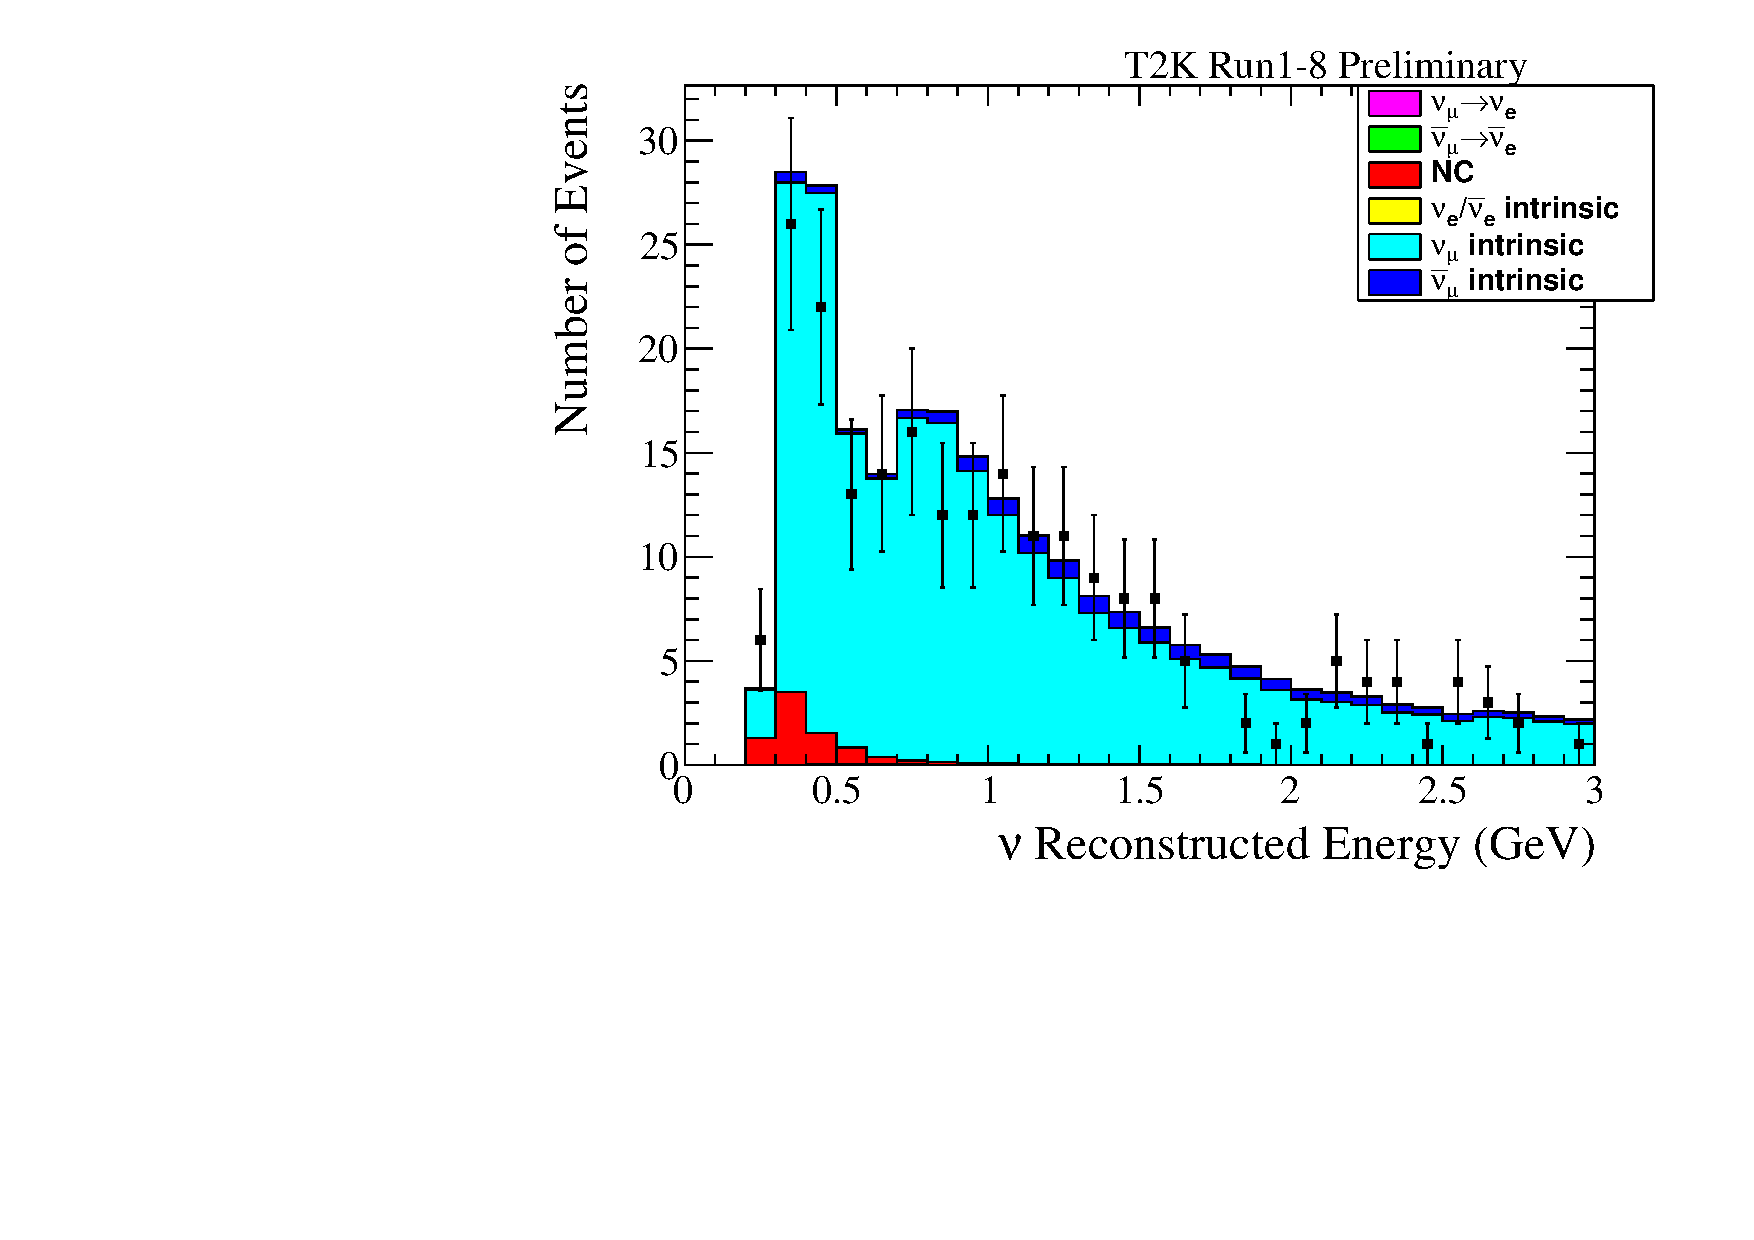
\includegraphics[width=0.9\textwidth]{spectra/2017b/spectrum_osc_asimovpf_1Rmu_data}
		\caption{Muon-like, neutrino mode}
	\end{subfigure}
	\begin{subfigure}[b]{0.49\textwidth}
		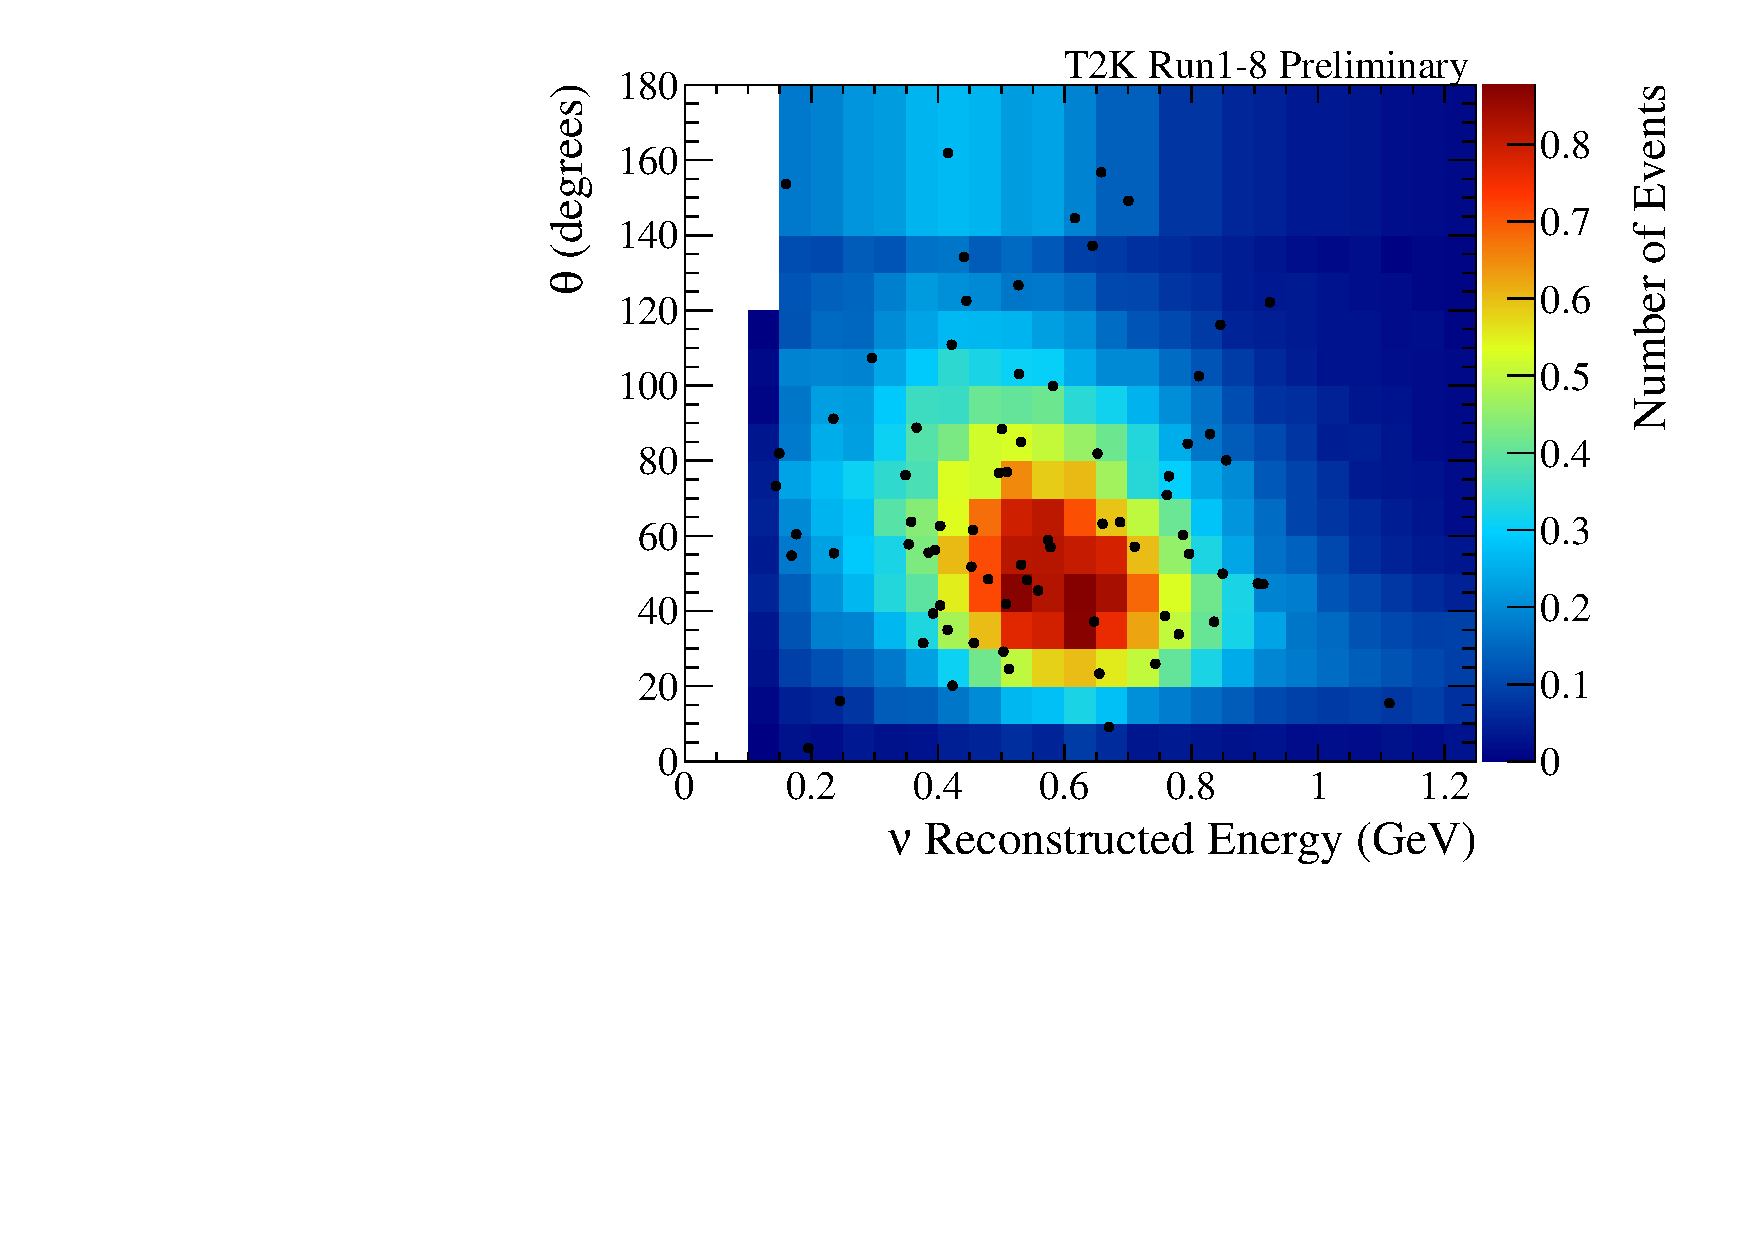
\includegraphics[width=0.9\textwidth]{spectra/2017b/spectrum_osc_asimovpf_1Re_data}
		\caption{Electron-like, neutrino mode}
	\end{subfigure}
	\begin{subfigure}[b]{0.49\textwidth}
		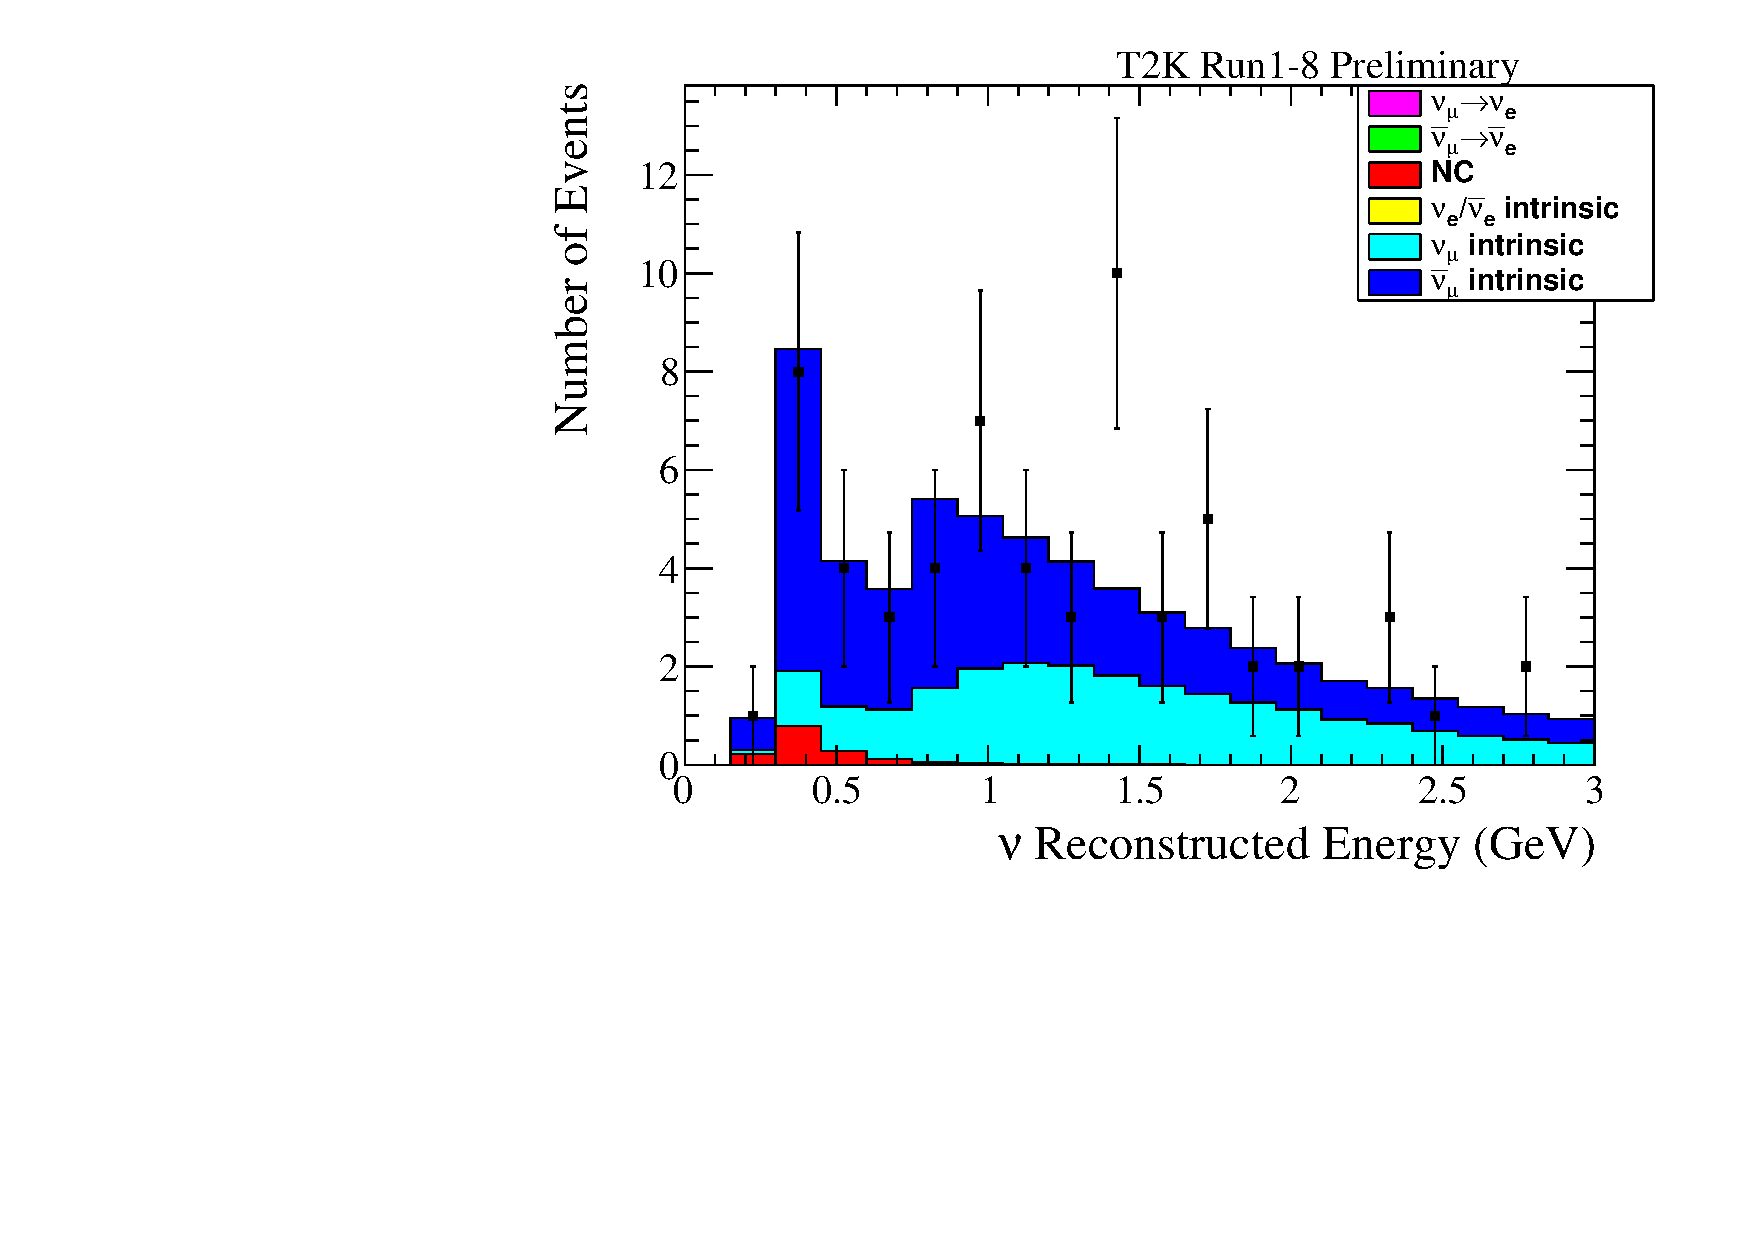
\includegraphics[width=0.9\textwidth]{spectra/2017b/spectrum_osc_asimovpf_RHC1Rmu_data}
		\caption{Muon-like, antineutrino mode}
	\end{subfigure}
	\begin{subfigure}[b]{0.49\textwidth}
		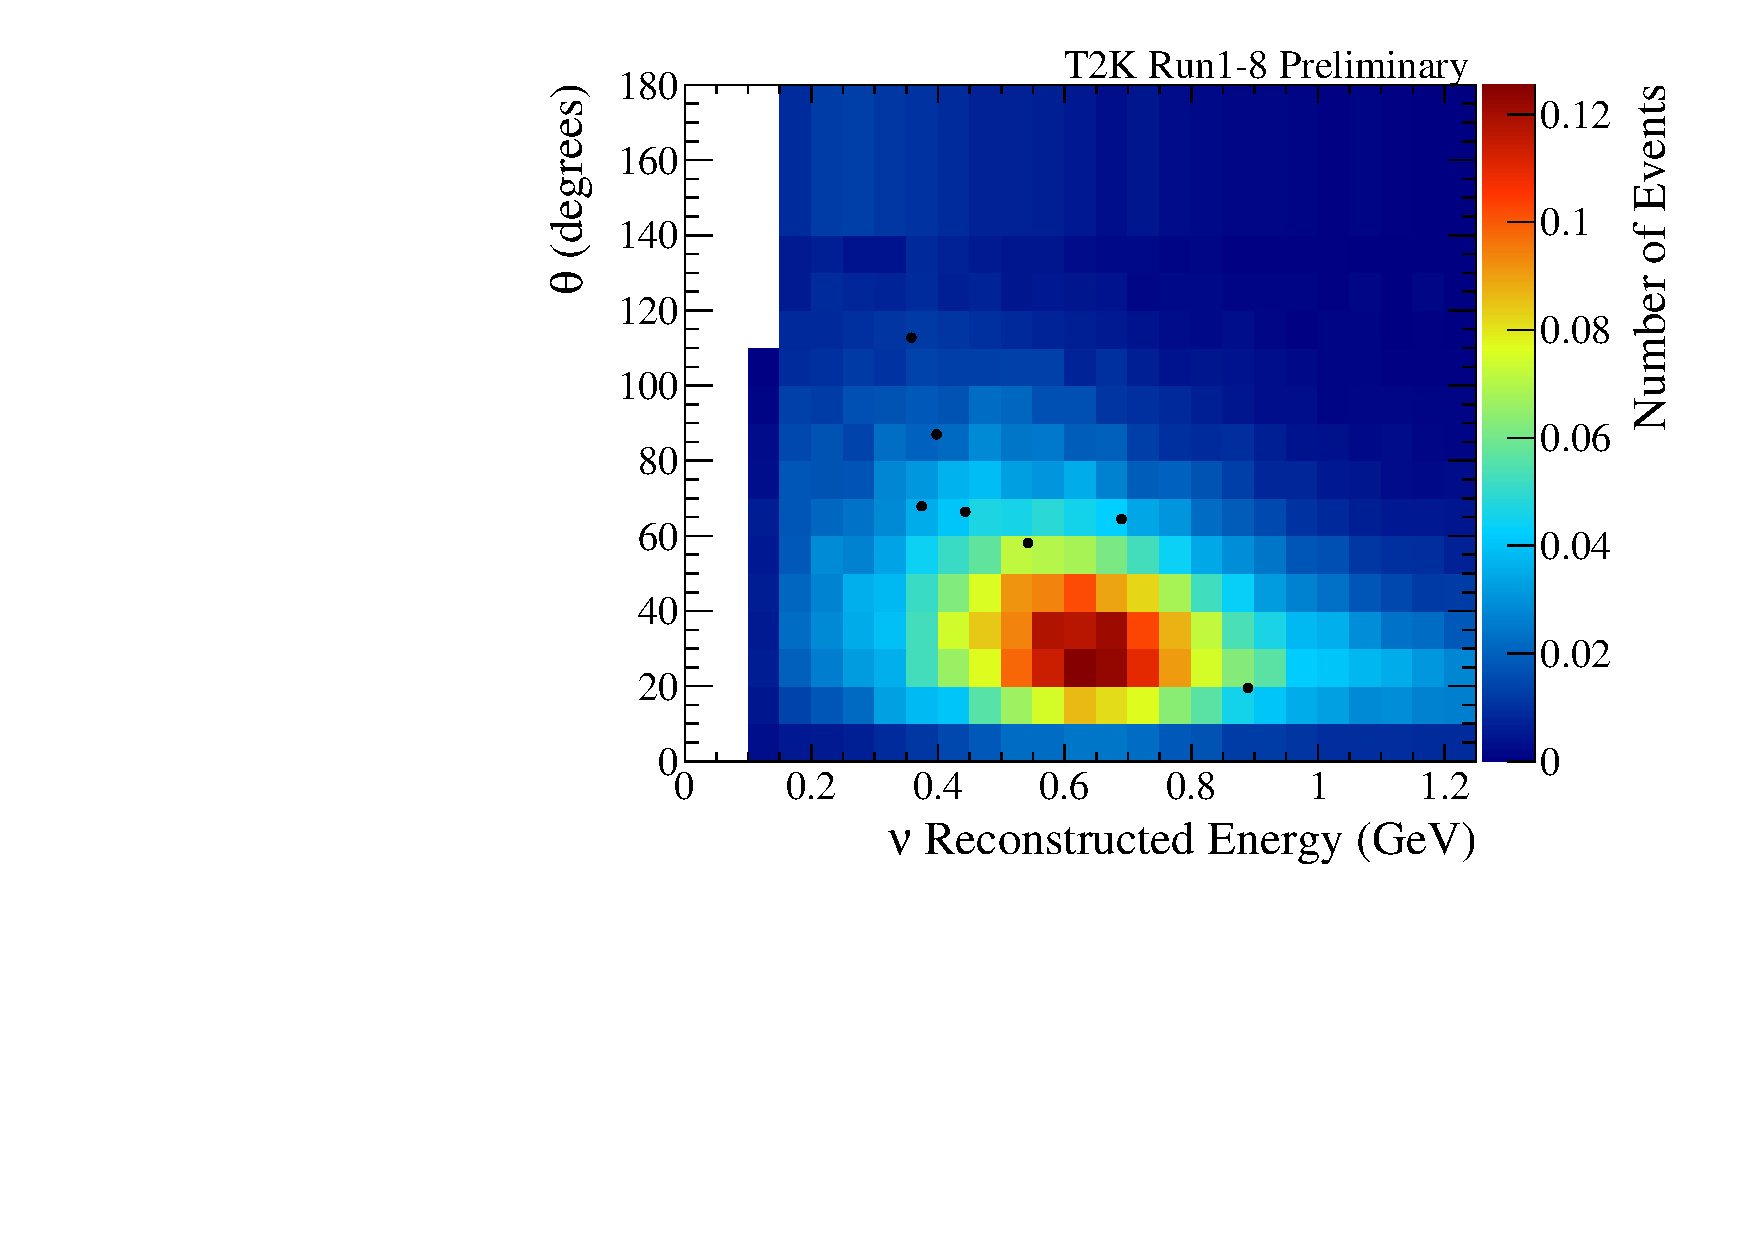
\includegraphics[width=0.9\textwidth]{spectra/2017b/spectrum_osc_asimovpf_RHC1Re_data}
		\caption{Electron-like antineutrino mode}
	\end{subfigure}
	\begin{subfigure}[b]{0.49\textwidth}
		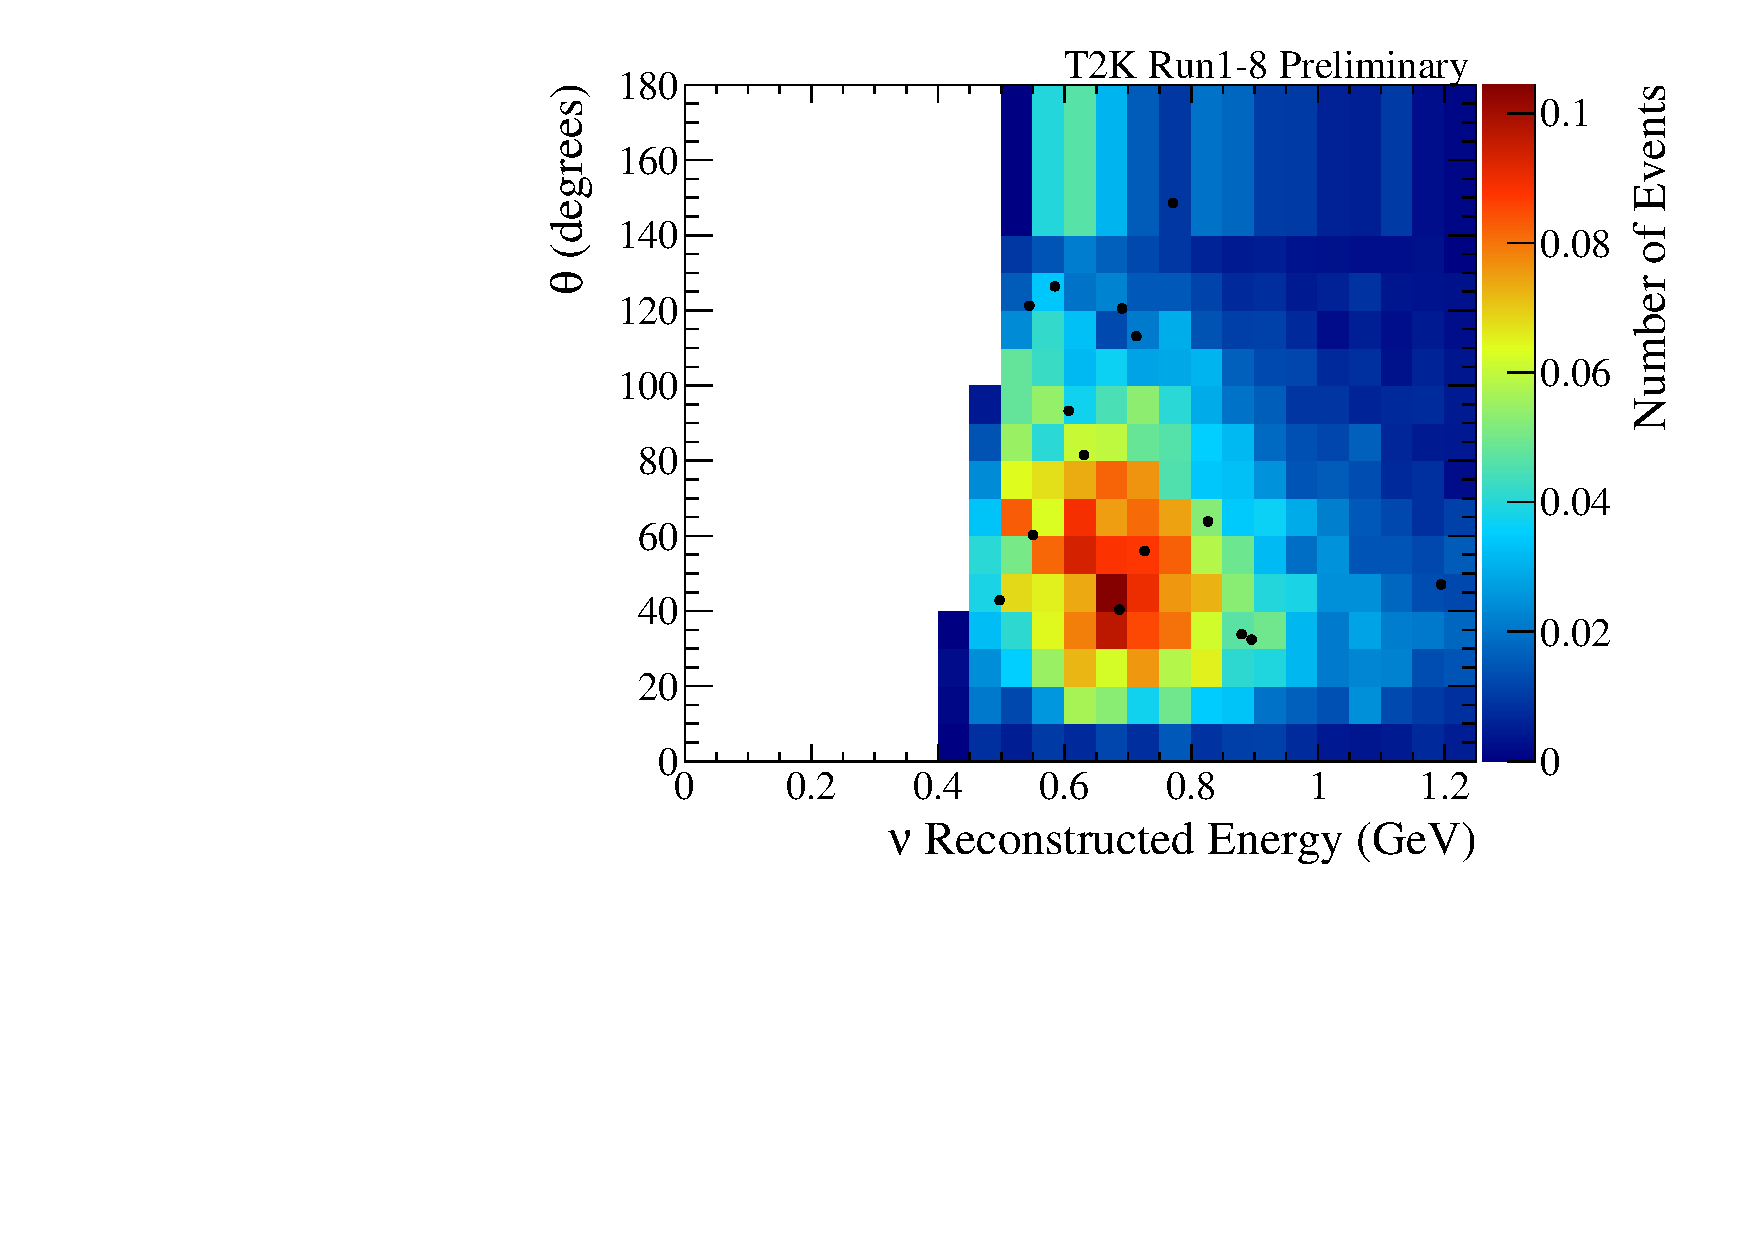
\includegraphics[width=0.9\textwidth]{spectra/2017b/spectrum_osc_asimovpf_MultiRe_data}
		\caption{\nueCConepi-like, neutrino mode}
	\end{subfigure}
	\caption {
		Predicted spectra and observed events (points). $\mu$-like distributions are a function of the reconstructed neutrino energy, while the $e$-like, including \nueCConepi, distributions are functions of both the reconstructed neutrino energy and the reconstructed angle between the outgoing lepton and the neutrino direction. The distributions correspond to the statistics collected in the full \RunPeriod data set. The spectra are generated with the systematic parameters described in \cref{sec:systematics} and the oscillation parameters corresponding to the best-fit values from the data fit (solar parameters at PDG 2016).
	}
	\label{fig:asimovpf_spectra_mc_data_2017b}
\end{figure*}
\clearpage
\begin{figure*}[htb]
	\center

	\begin{subfigure}[b]{0.49\textwidth}
		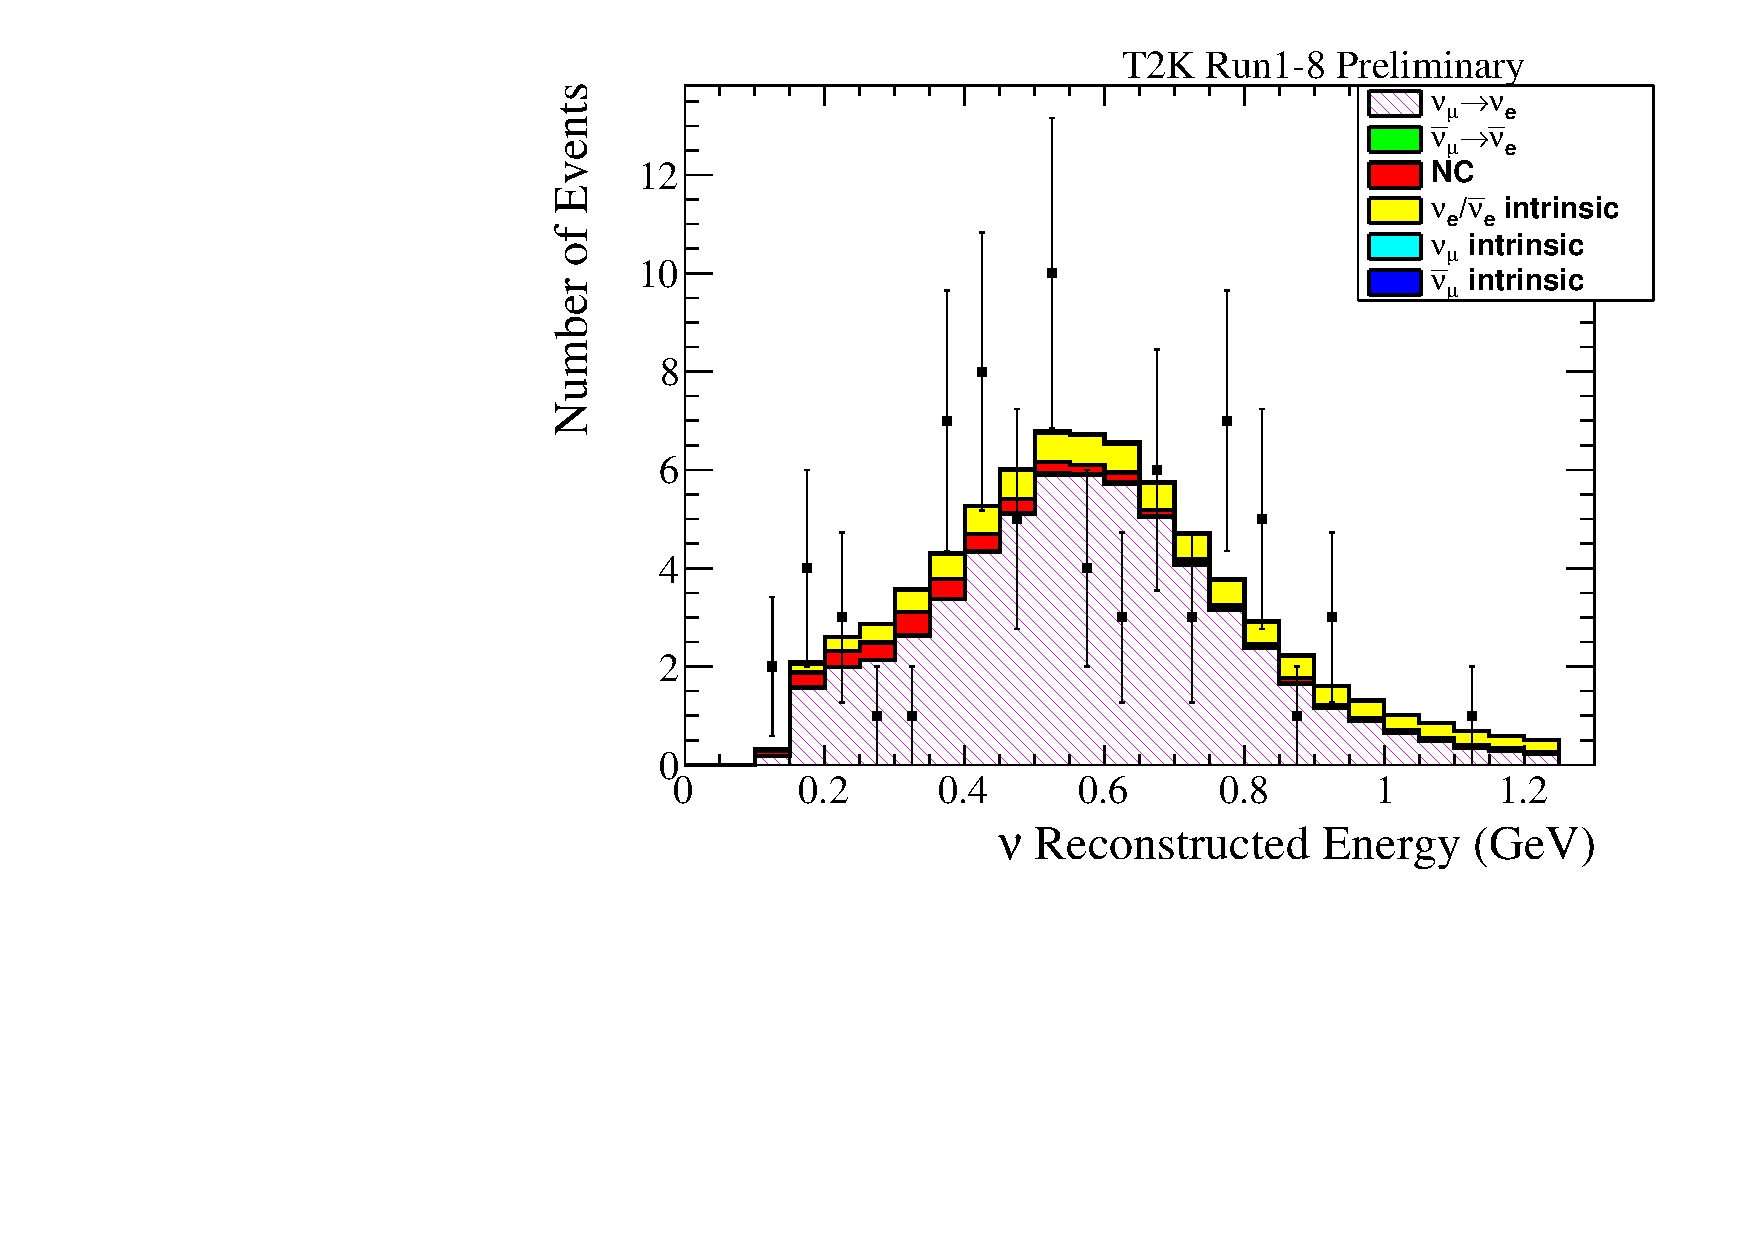
\includegraphics[width=0.9\textwidth]{spectra/2017b/erec_spectrum_osc_asimovpf_1Re_data}
		\caption{Electron-like, neutrino mode}
	\end{subfigure}
	\begin{subfigure}[b]{0.49\textwidth}
		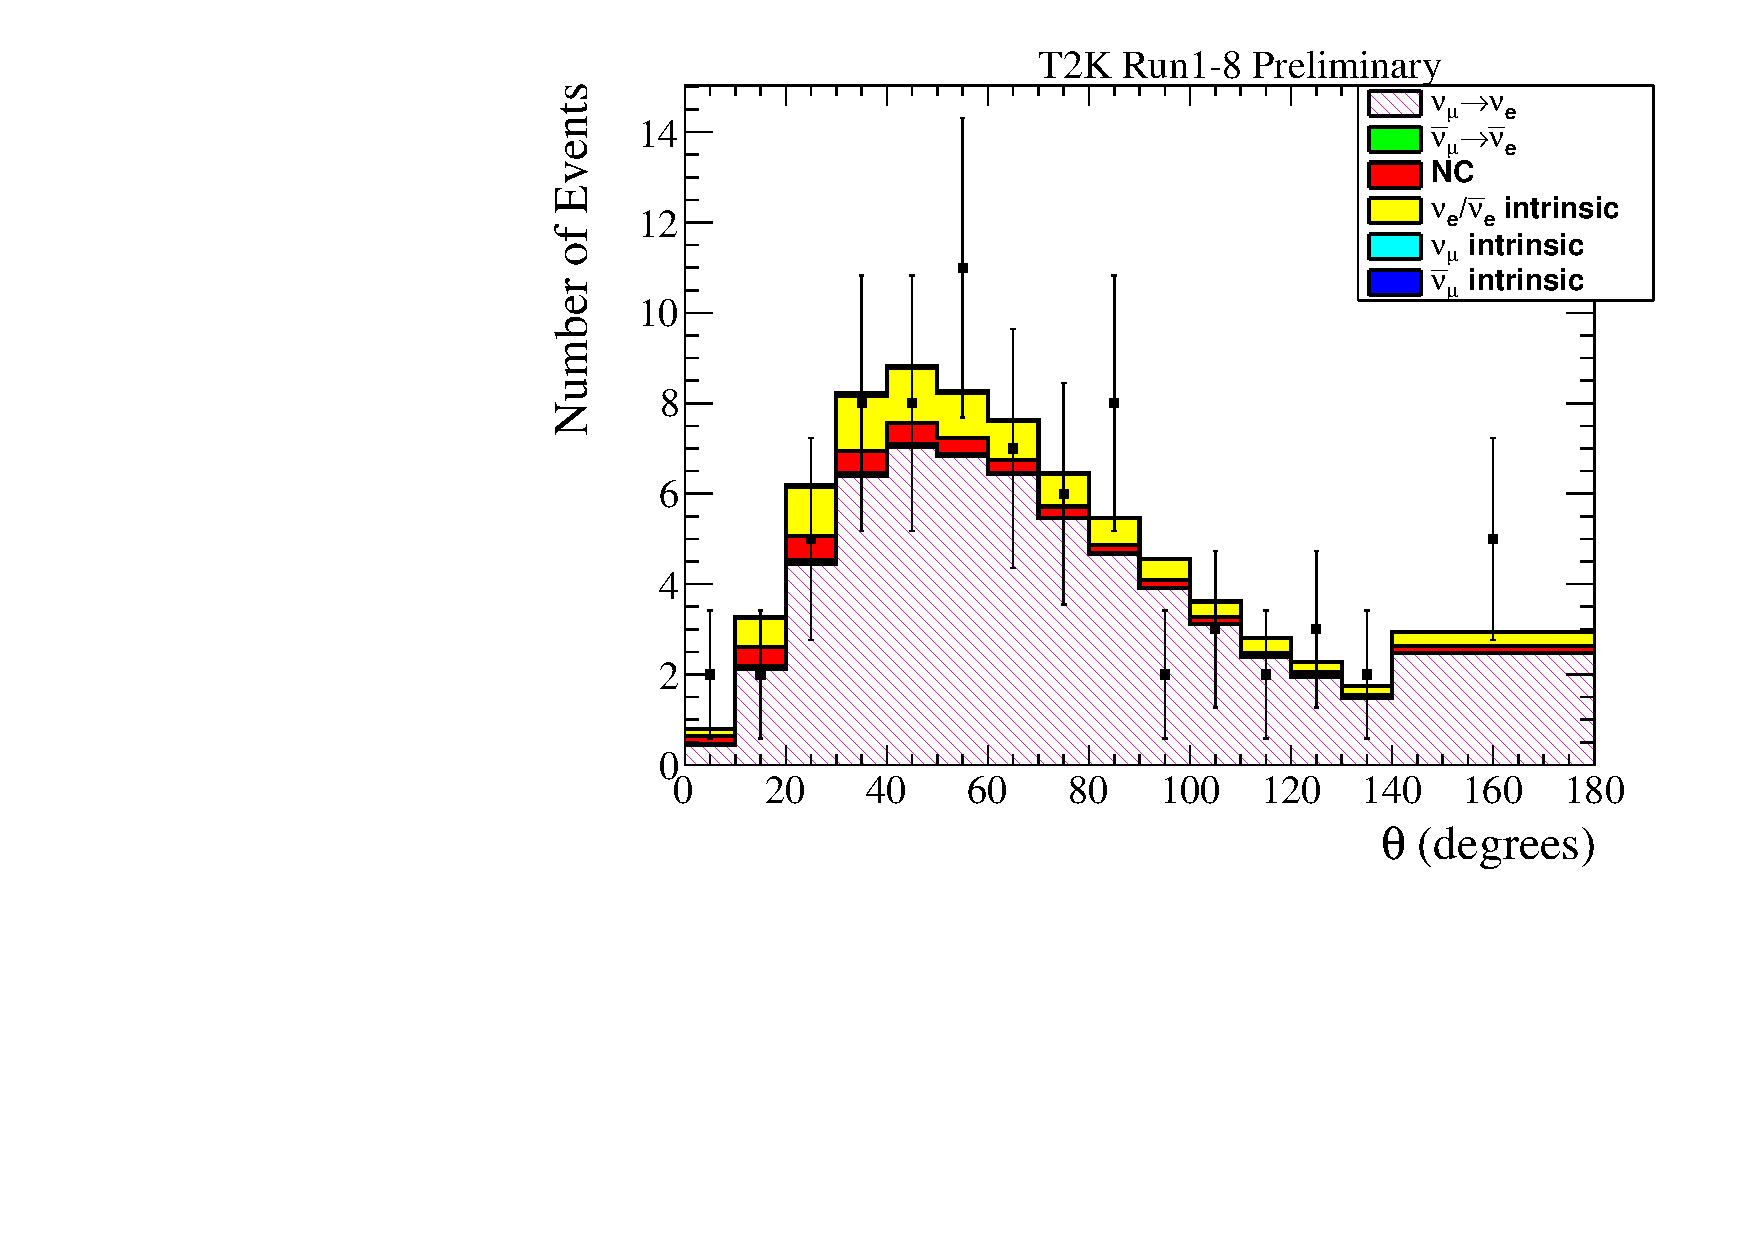
\includegraphics[width=0.9\textwidth]{spectra/2017b/theta_spectrum_osc_asimovpf_1Re_data}
		\caption{Electron-like, neutrino mode}
	\end{subfigure}

	\begin{subfigure}[b]{0.49\textwidth}
		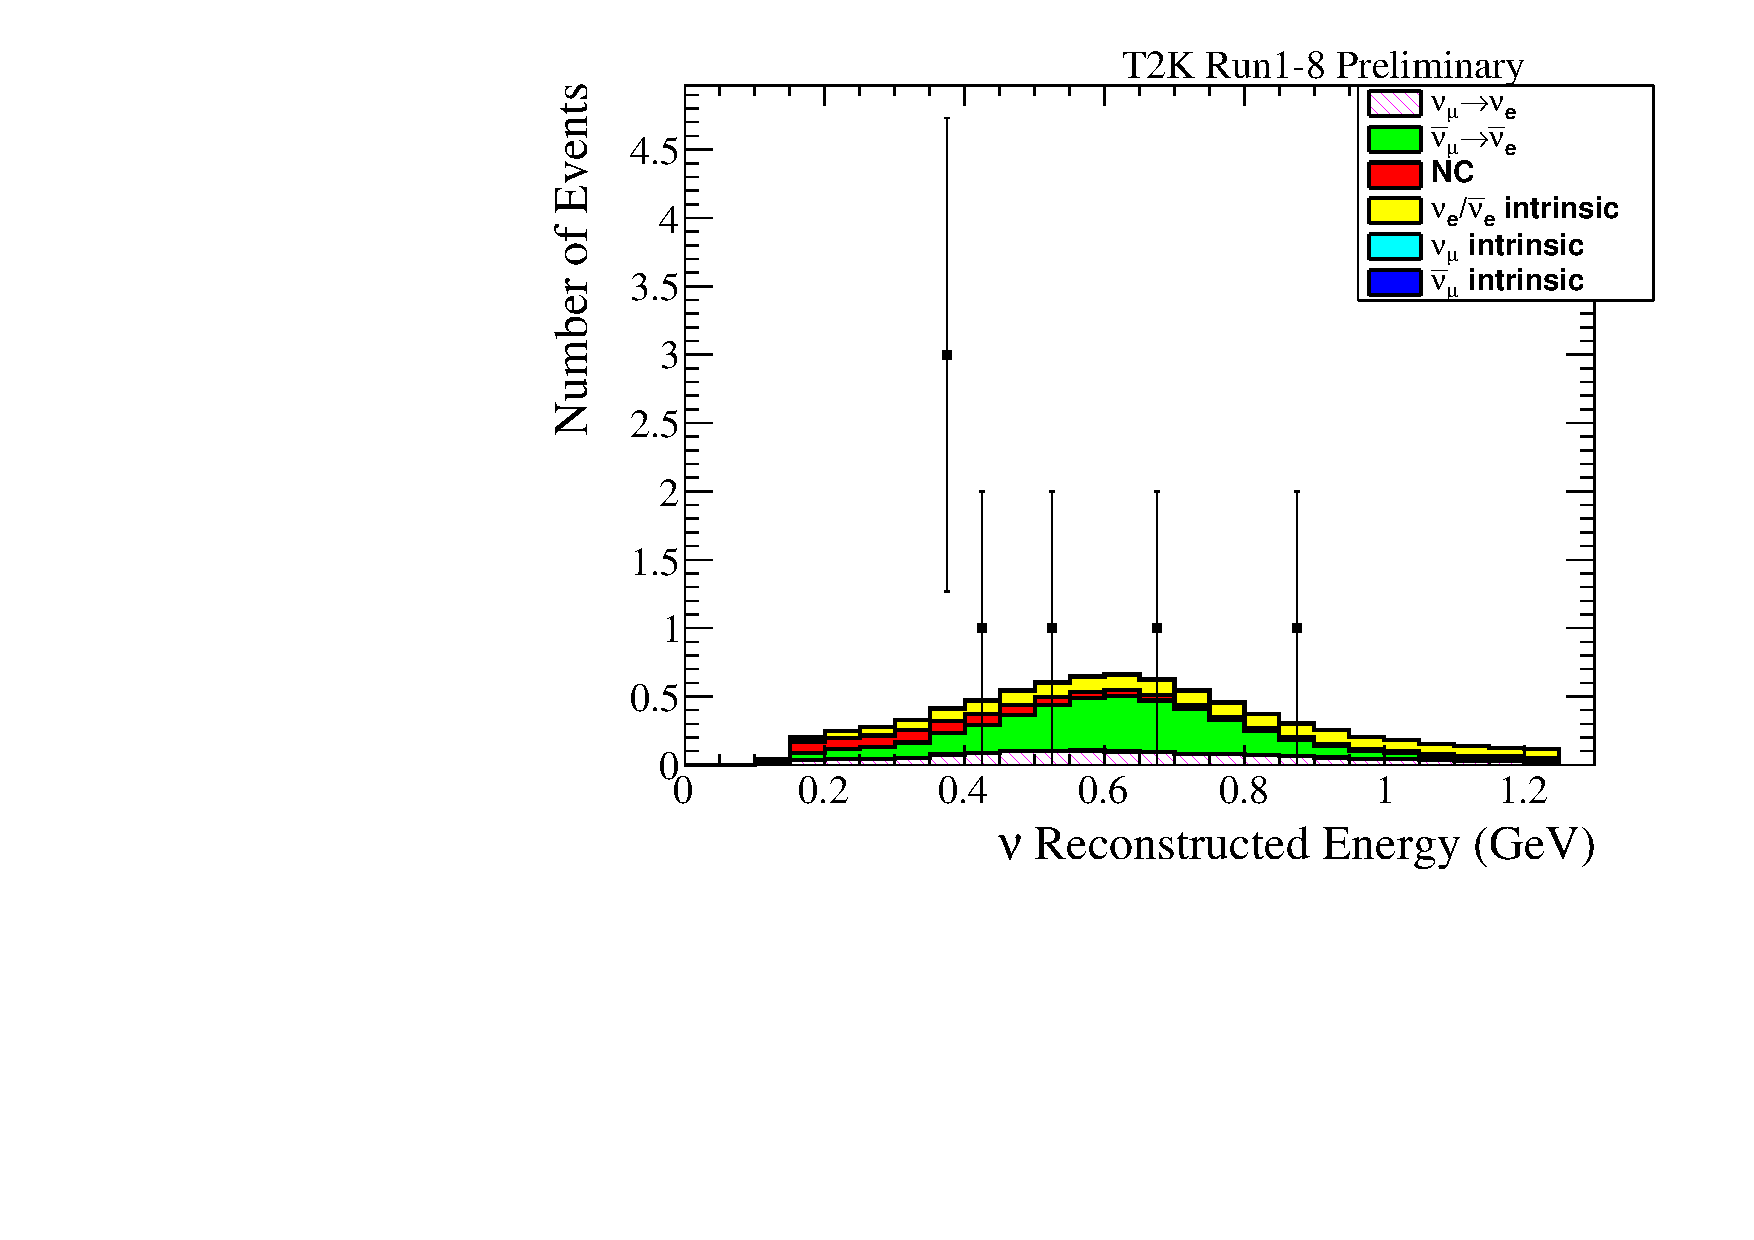
\includegraphics[width=0.9\textwidth]{spectra/2017b/erec_spectrum_osc_asimovpf_RHC1Re_data}
		\caption{Electron-like antineutrino mode}
	\end{subfigure}
	\begin{subfigure}[b]{0.49\textwidth}
		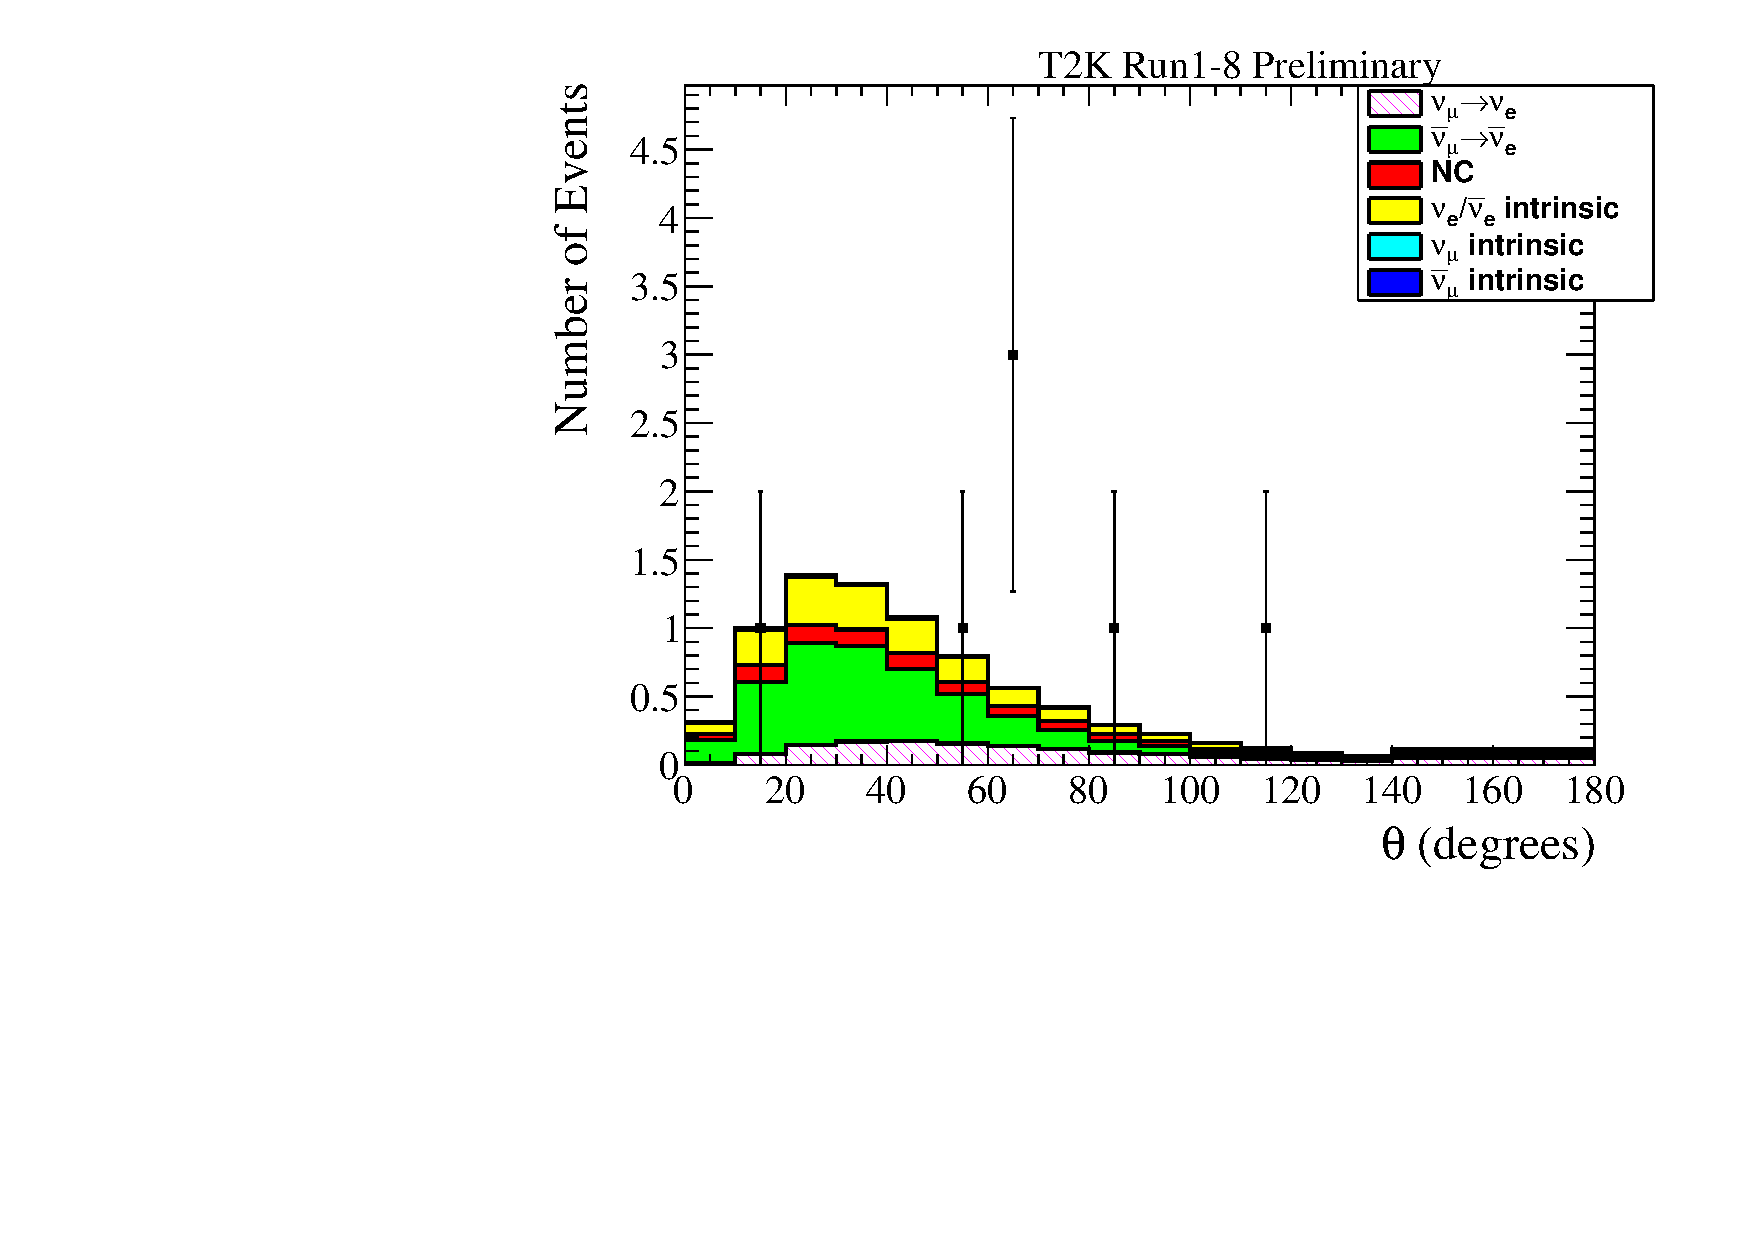
\includegraphics[width=0.9\textwidth]{spectra/2017b/theta_spectrum_osc_asimovpf_RHC1Re_data}
		\caption{Electron-like antineutrino mode}
	\end{subfigure}

	\begin{subfigure}[b]{0.49\textwidth}
		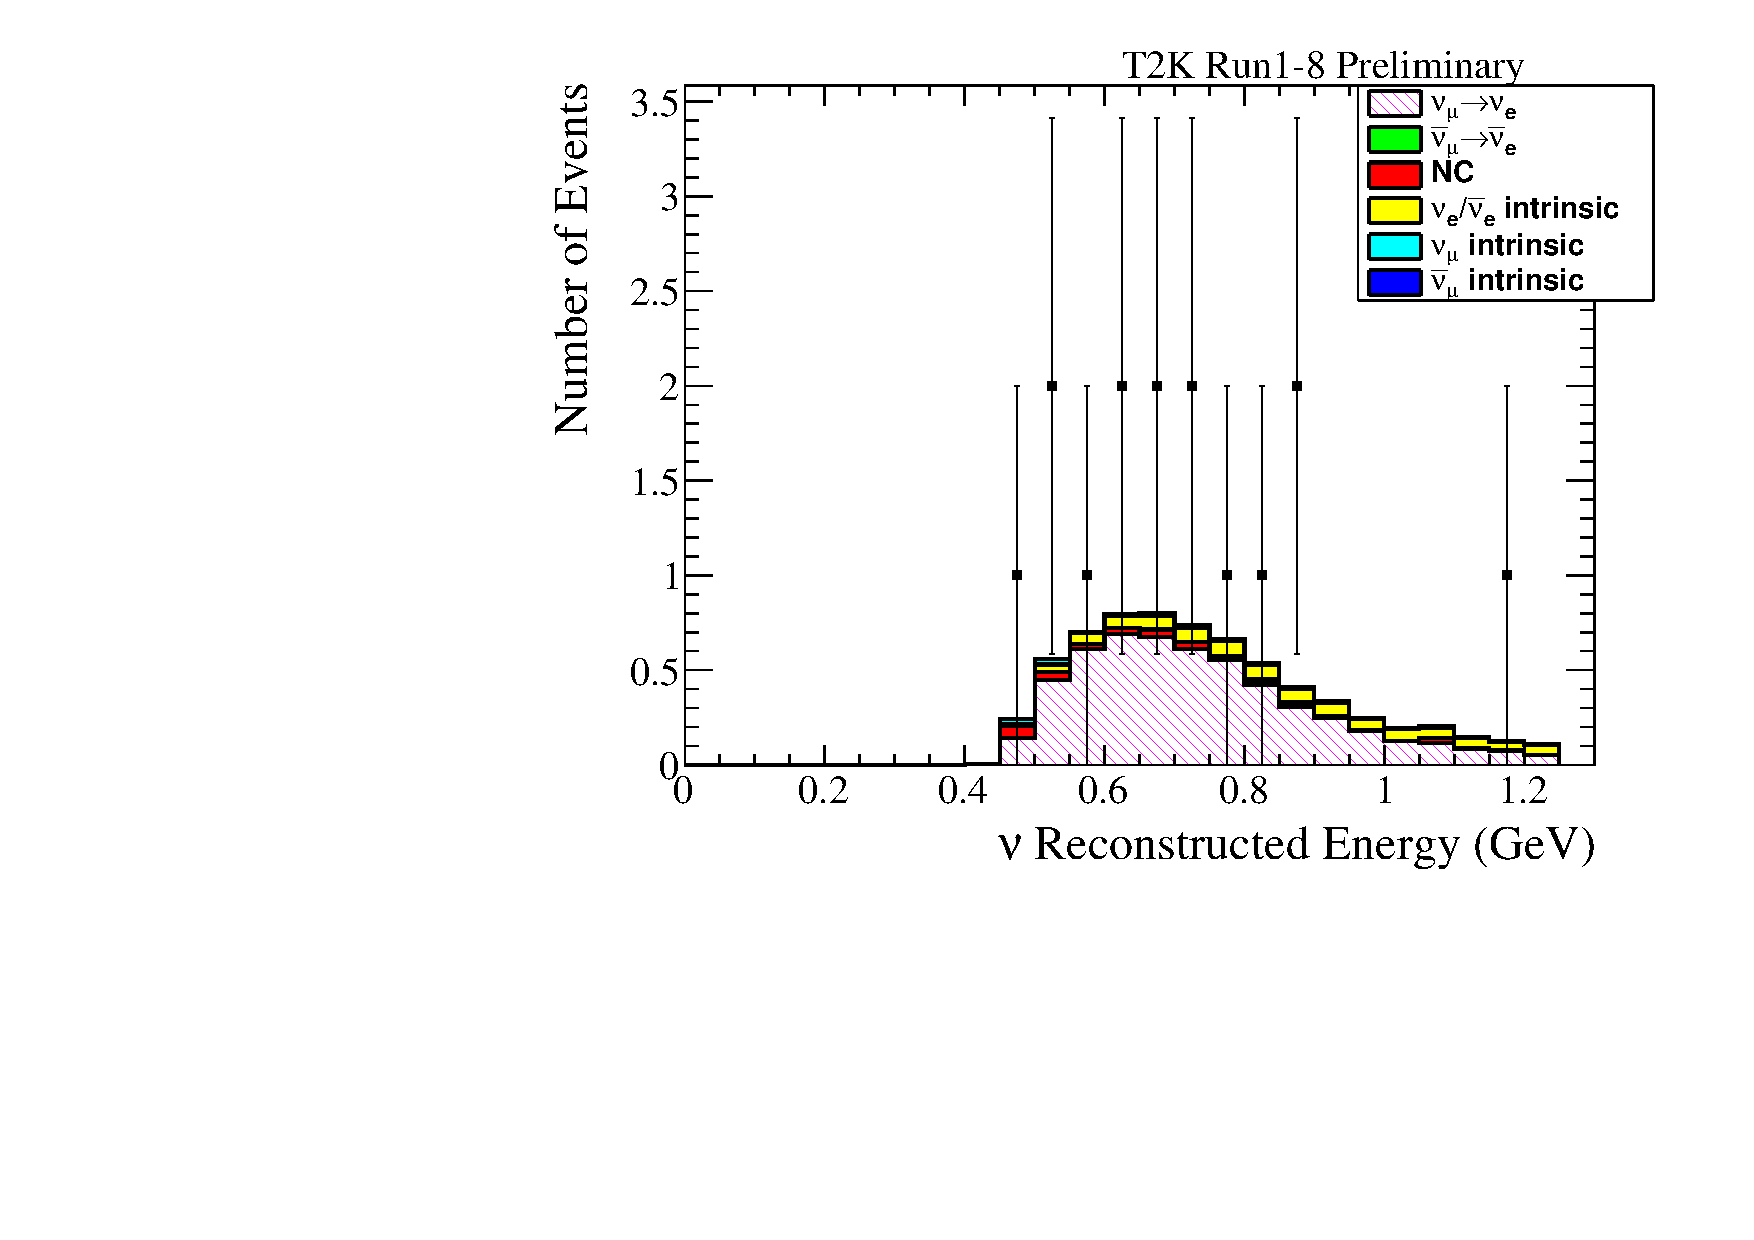
\includegraphics[width=0.9\textwidth]{spectra/2017b/erec_spectrum_osc_asimovpf_MultiRe_data}
		\caption{\nueCConepi-like, neutrino mode}
	\end{subfigure}
	\begin{subfigure}[b]{0.49\textwidth}
		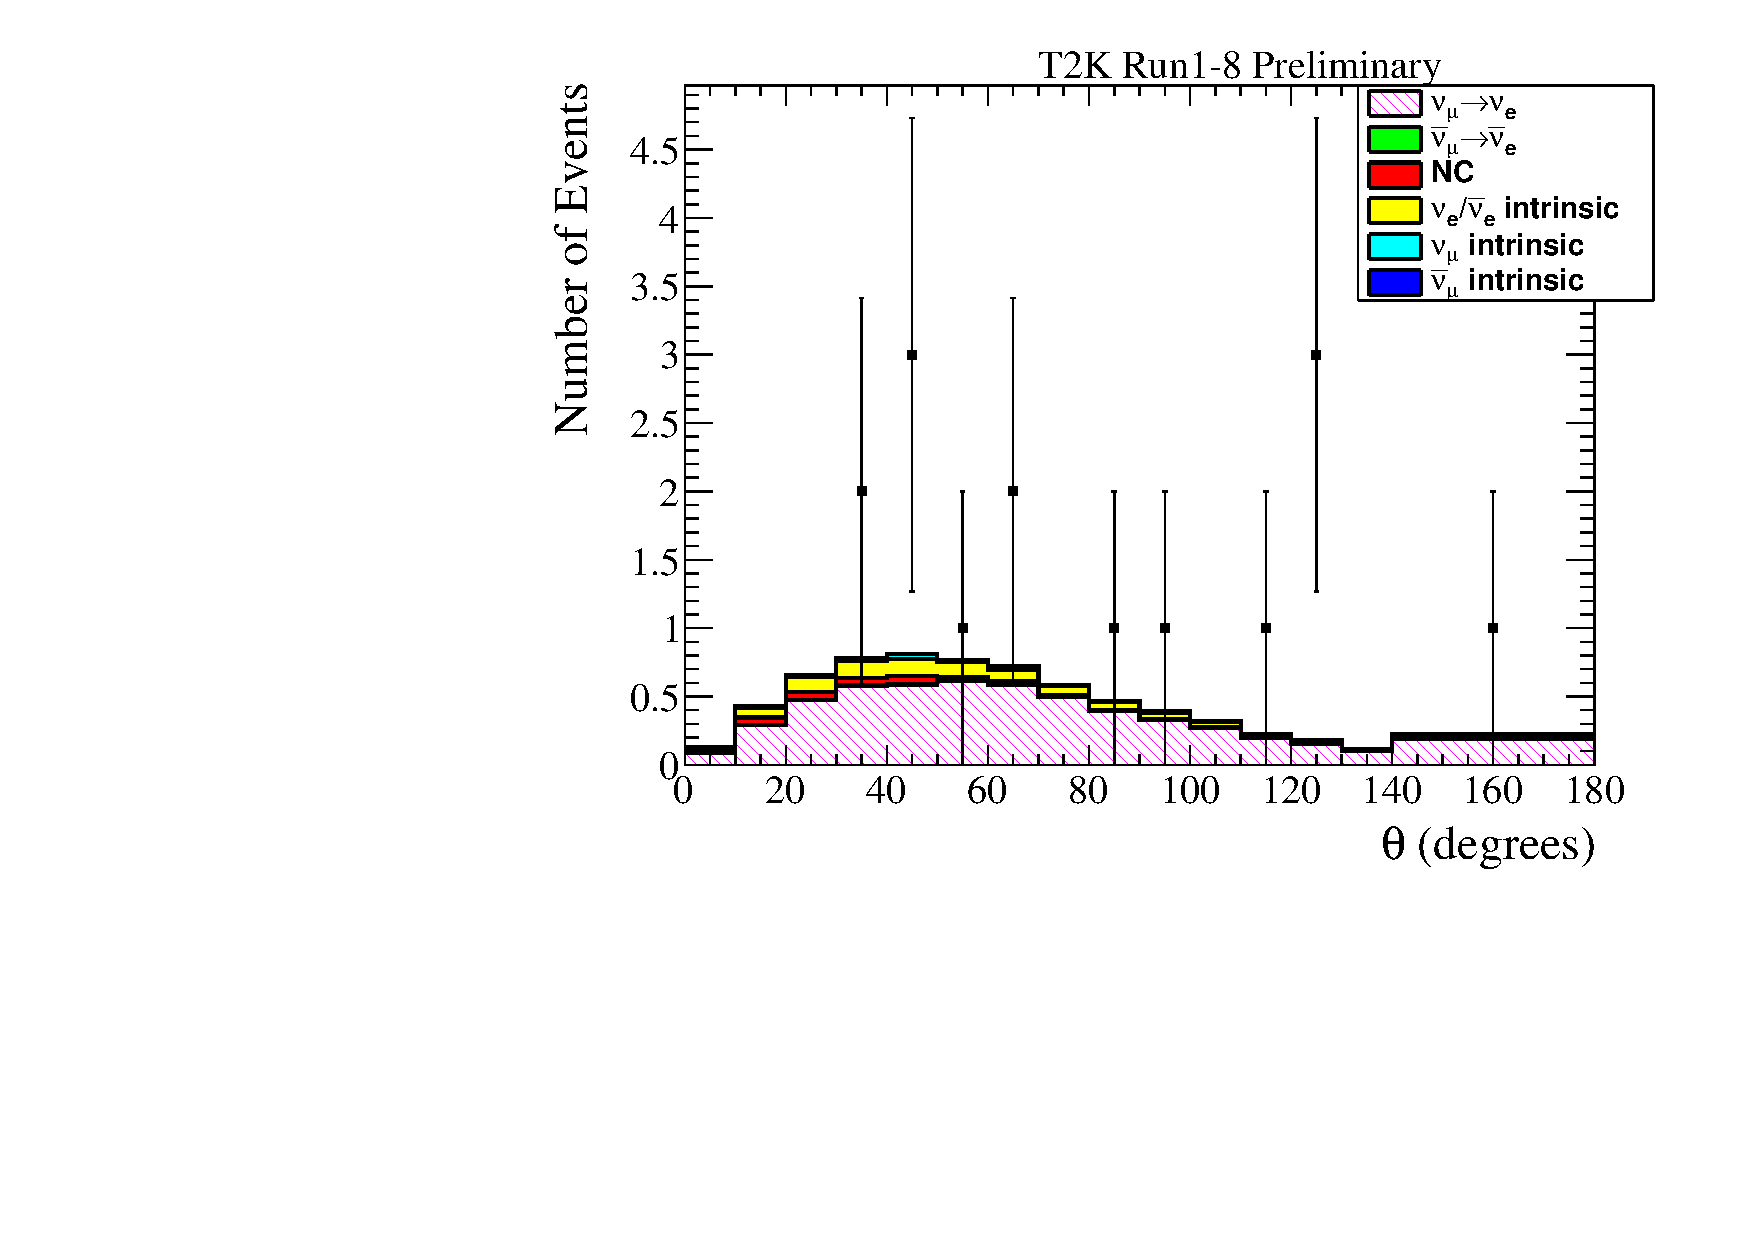
\includegraphics[width=0.9\textwidth]{spectra/2017b/theta_spectrum_osc_asimovpf_MultiRe_data}
		\caption{\nueCConepi-like, neutrino mode}
	\end{subfigure}
	\caption {
		Predicted spectra and observed events (points). The $e$-like, including \nueCConepi, distributions are functions of both the reconstructed neutrino energy and the reconstructed angle between the outgoing lepton and the neutrino direction, with the projections in each variable shown here. The distributions correspond to the statistics collected in the full \RunPeriod data set. The spectra are generated with the systematic parameters described in \cref{sec:systematics} and the oscillation parameters corresponding to the best-fit values from the data fit (solar parameters at PDG 2016).
	}
	\label{fig:asimovpf_spectra_mc_data_elike_1D_2017b}
\end{figure*}
\clearpage

The best-fit values and $1\sigma$ ranges for each oscillation parameter are shown in \cref{tab:data_bestfit_2017b} for normal hierarchy (which is preferred in all data fits). The $1\sigma$ ranges are extracted for each oscillation parameter from the 1-dimensional $\Delta \chi^2$ distributions shown in \crefrange{fig:dcp_data_2017b}{fig:dmsq23_data_2017b}.

The 1-dimensional contours are plotted with respect to the global minimum from normal and inverted hierarchies, while the 2-dimensional confidence intervals are shown drawing the normal and inverted hierarchy contours independently, i.e. each contour is produced with respect to the global minimum under that hierarchy hypothesis.

\begin{table}
\centering
\begin{tabular}{| c | c | c | c | c | c |}
\hline
Parameter & Reactor & Best-fit (NH) & $\pm1\sigma$ (NH) & Best-fit (IH) & $\pm1\sigma$ (IH) \\
\hline
\deltacp & Yes & \BestFitDeltacpwRCb & [\MOneSigmaDeltacpwRCb,\POneSigmaDeltacpwRCb] & \BestFitDeltacpwRCIHb & [\MOneSigmaDeltacpwRCIHb,\POneSigmaDeltacpwRCIHb] \\
\deltacp & No & \BestFitDeltacpwoRCb & [\MOneSigmaDeltacpwoRCb,\POneSigmaDeltacpwoRCb] & \BestFitDeltacpwoRCIHb & [\MOneSigmaDeltacpwoRCIHb,\POneSigmaDeltacpwoRCIHb] \\
\ssqthonethree & No & \BestFitMixingOneThreewoRCb & [\MOneMixingOneThreewoRCb,\POneMixingOneThreewoRCb] & \BestFitMixingOneThreewoRCIHb & [\MOneMixingOneThreewoRCIHb,\POneMixingOneThreewoRCIHb] \\
\ssqthtwothree & Yes & \BestFitMixingTwoThreewRCb & [\MOneMixingTwoThreewRCb,\POneMixingTwoThreewRCb] & \BestFitMixingTwoThreewRCIHb & [\MOneMixingTwoThreewRCIHb,\POneMixingTwoThreewRCIHb] \\
\dmsqtwothree or \dmsqonethree & Yes & \BestFitDmTwoThreewRCb & [\MOneDmTwoThreewRCb,\POneDmTwoThreewRCb] & \BestFitDmTwoThreewRCIHb & [\MOneDmTwoThreewRCIHb,\POneDmTwoThreewRCIHb] \\
 ($10^{-3}\text{ eV}^2\text{/c}^4$) & & & & & \\
\hline
\end{tabular}

\caption{
The \RunPeriod measured oscillation parameter best-fit and the $\pm 1\sigma$ intervals are shown for normal and inverted hierarchies with respect to the hierarchy best-fit. The $\pm 1\sigma$ interval is obtained by using the constant $\Delta \chi^2$ method. For each parameter normal hierarchy is the global best-fit.
}
\label{tab:data_bestfit_2017b}
\end{table}

\clearpage

\subsubsection{Results for \appearance}
In \cref{fig:ssqth13_vs_dcp_data_2017b} the result for \appearance with reactor constraint and T2K only is shown.

\begin{figure*}[htb]
	\center
	\begin{subfigure}[b]{0.49\textwidth}
		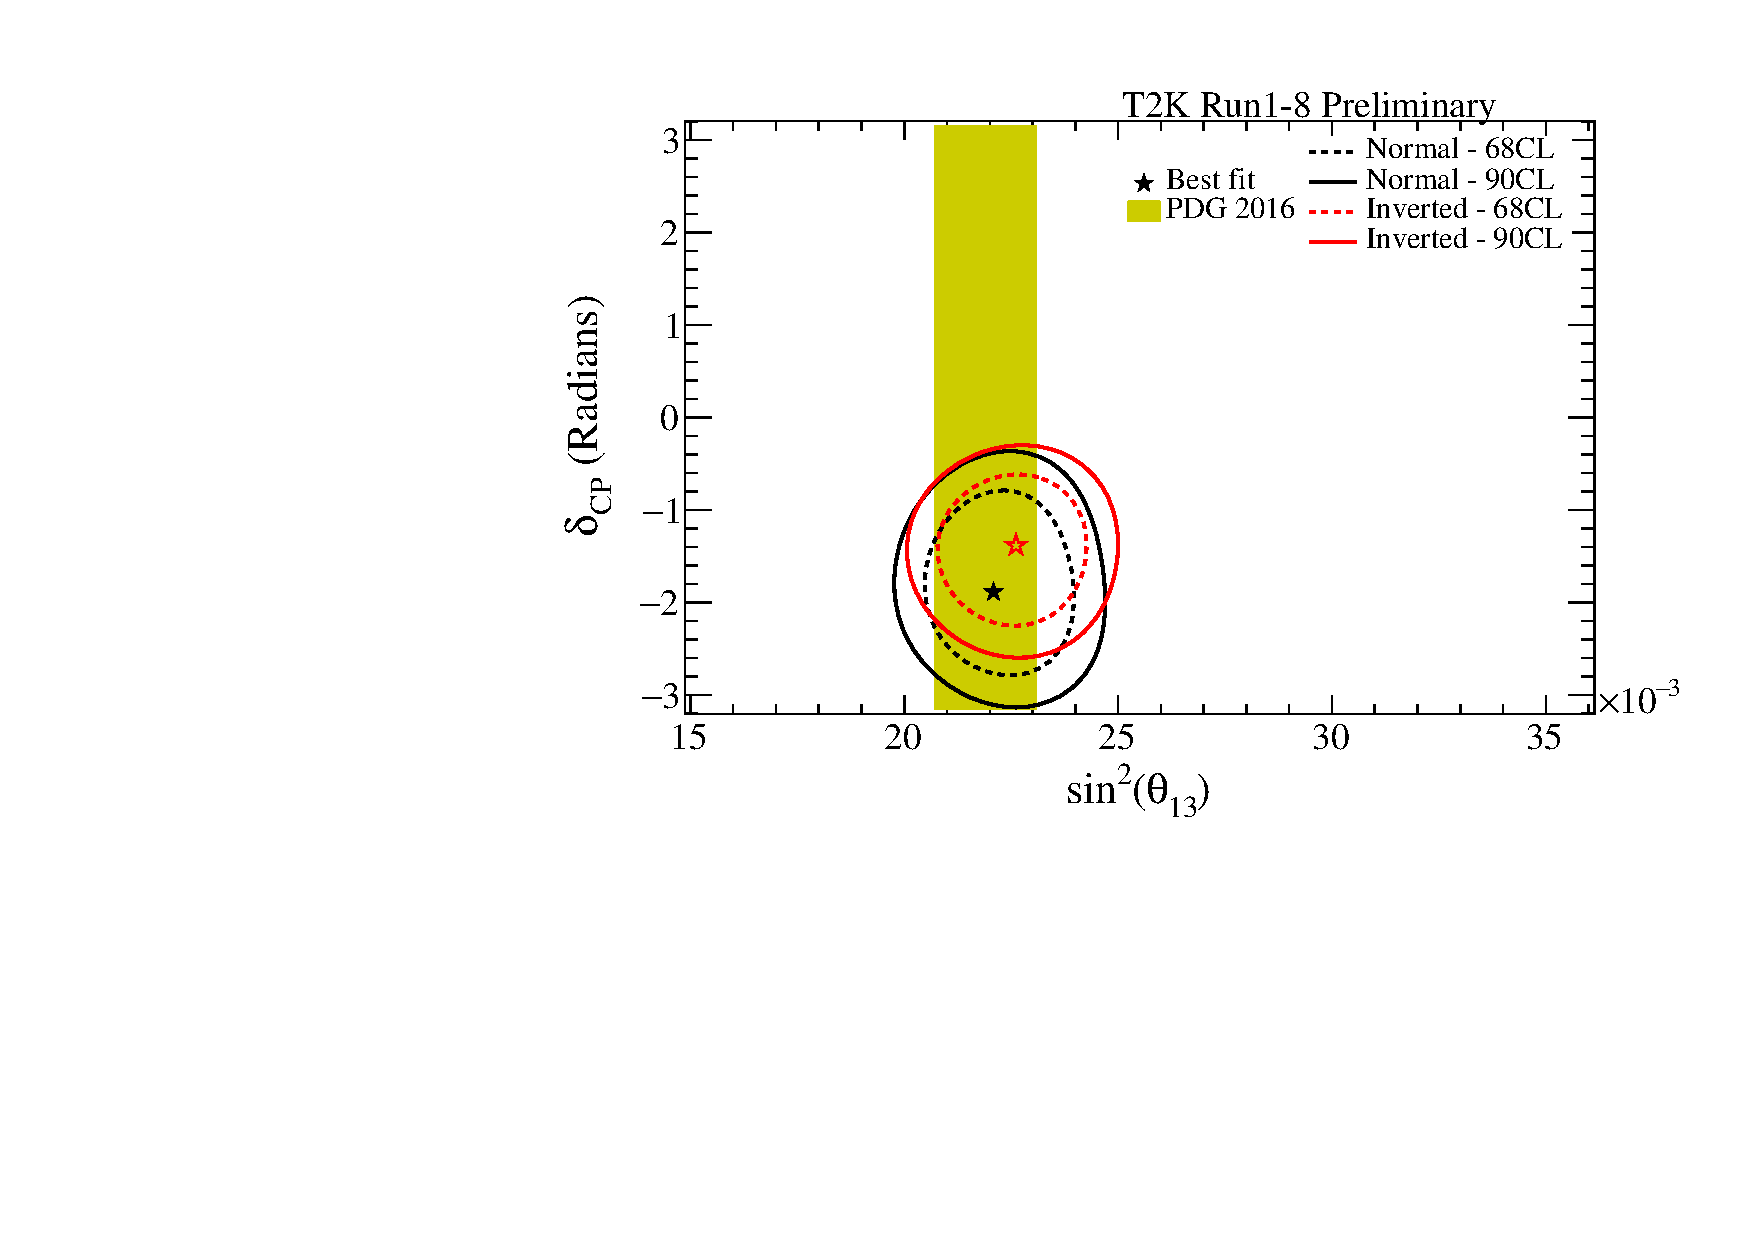
\includegraphics[width=0.9\textwidth]{data/reactor/2017b/mixing13_deltacp_data_reactor_global}
		\caption{\appearance with reactor constraint}
	\end{subfigure}
	\begin{subfigure}[b]{0.49\textwidth}
		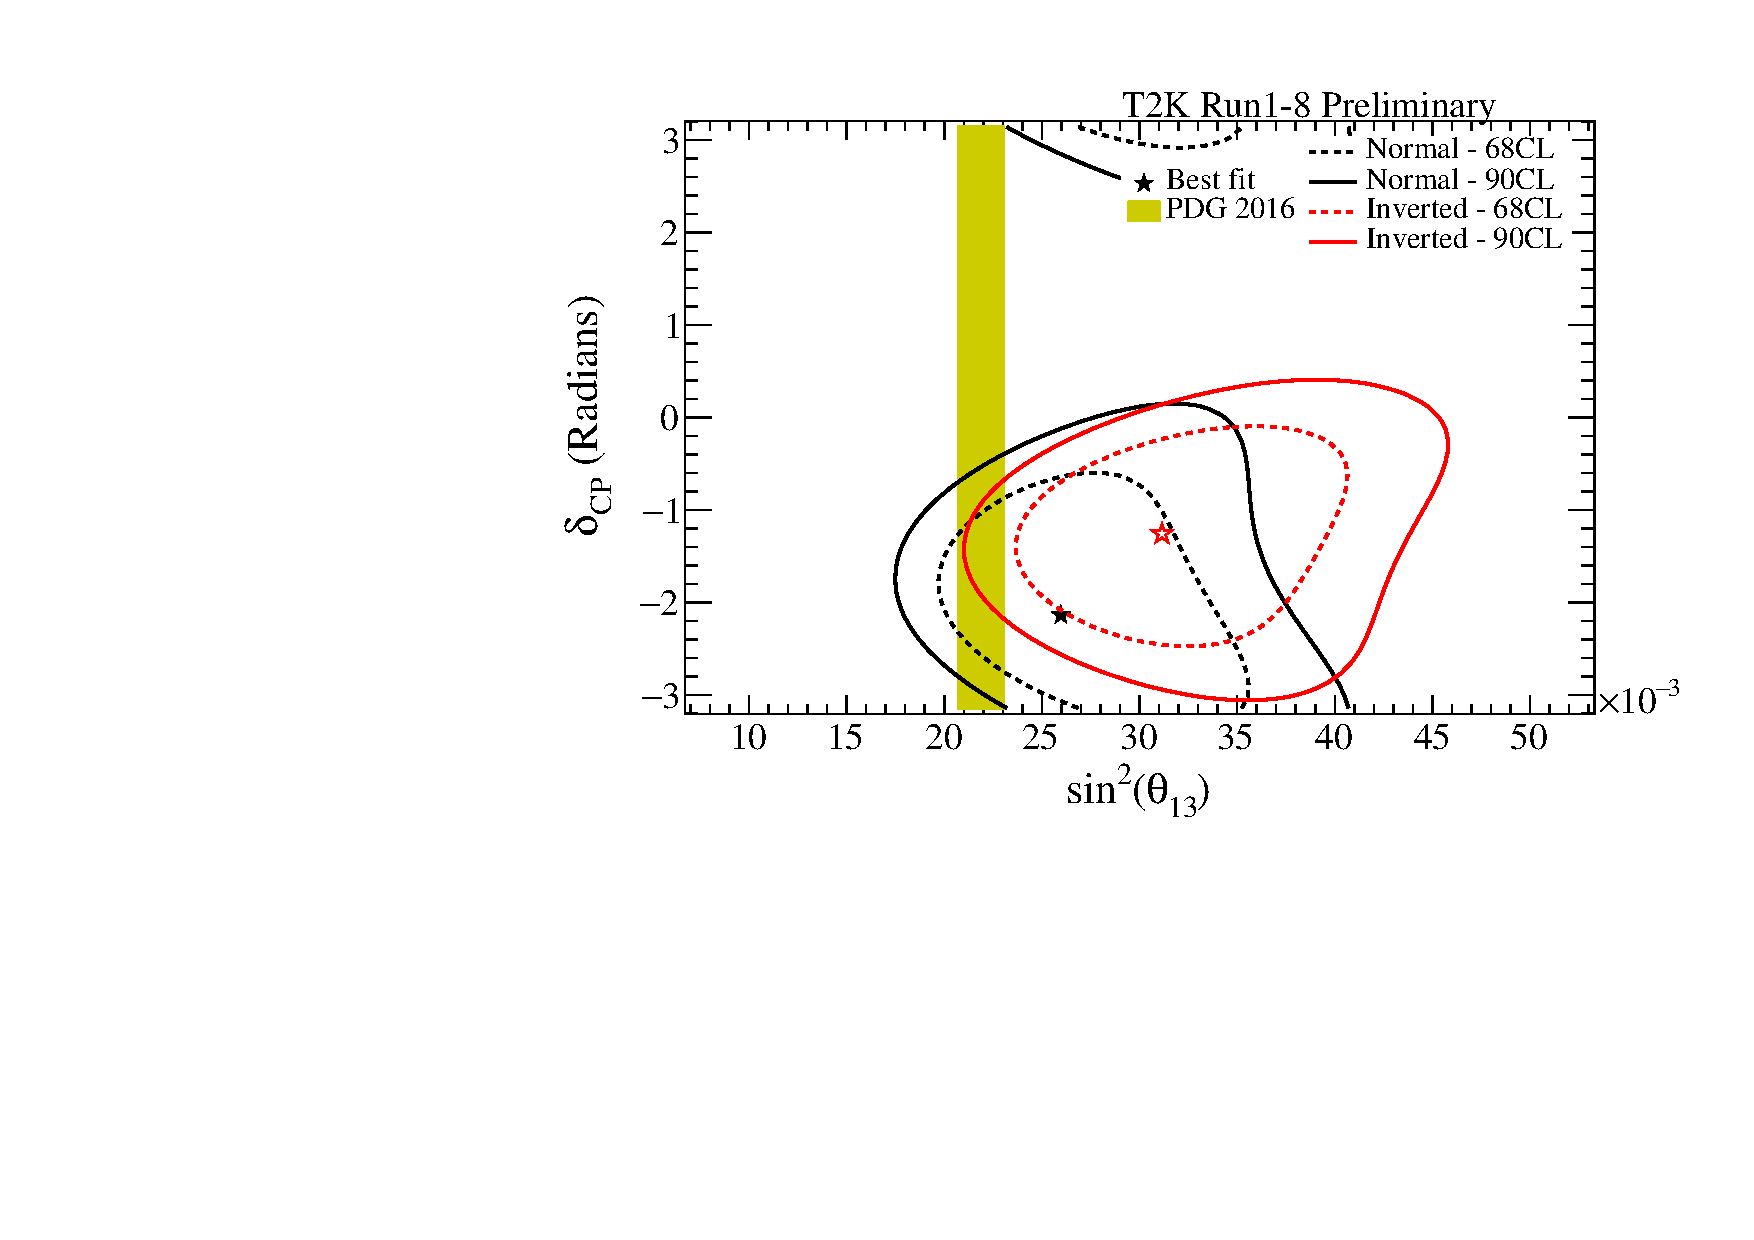
\includegraphics[width=0.9\textwidth]{data/t2k/2017b/mixing13_deltacp_data_t2k_global}
		\caption{\appearance T2K only}
	\end{subfigure}
	\caption {
		Contours at 68\% and 90\% CL for \appearance with and without reactor constraint. Normal and inverted hierarchy contours are independent. All 5 samples were used to produce these fits.
	}
	\label{fig:ssqth13_vs_dcp_data_2017b}
\end{figure*}

\subsubsection{Results for \disappearance}

The result for \disappearance with reactor constraint and T2K only is shown in fig.~\ref{fig:ssqth23_vs_dmsq23_data_2017b}.

\begin{figure*}[htb]
	\center
	\begin{subfigure}[b]{0.49\textwidth}
		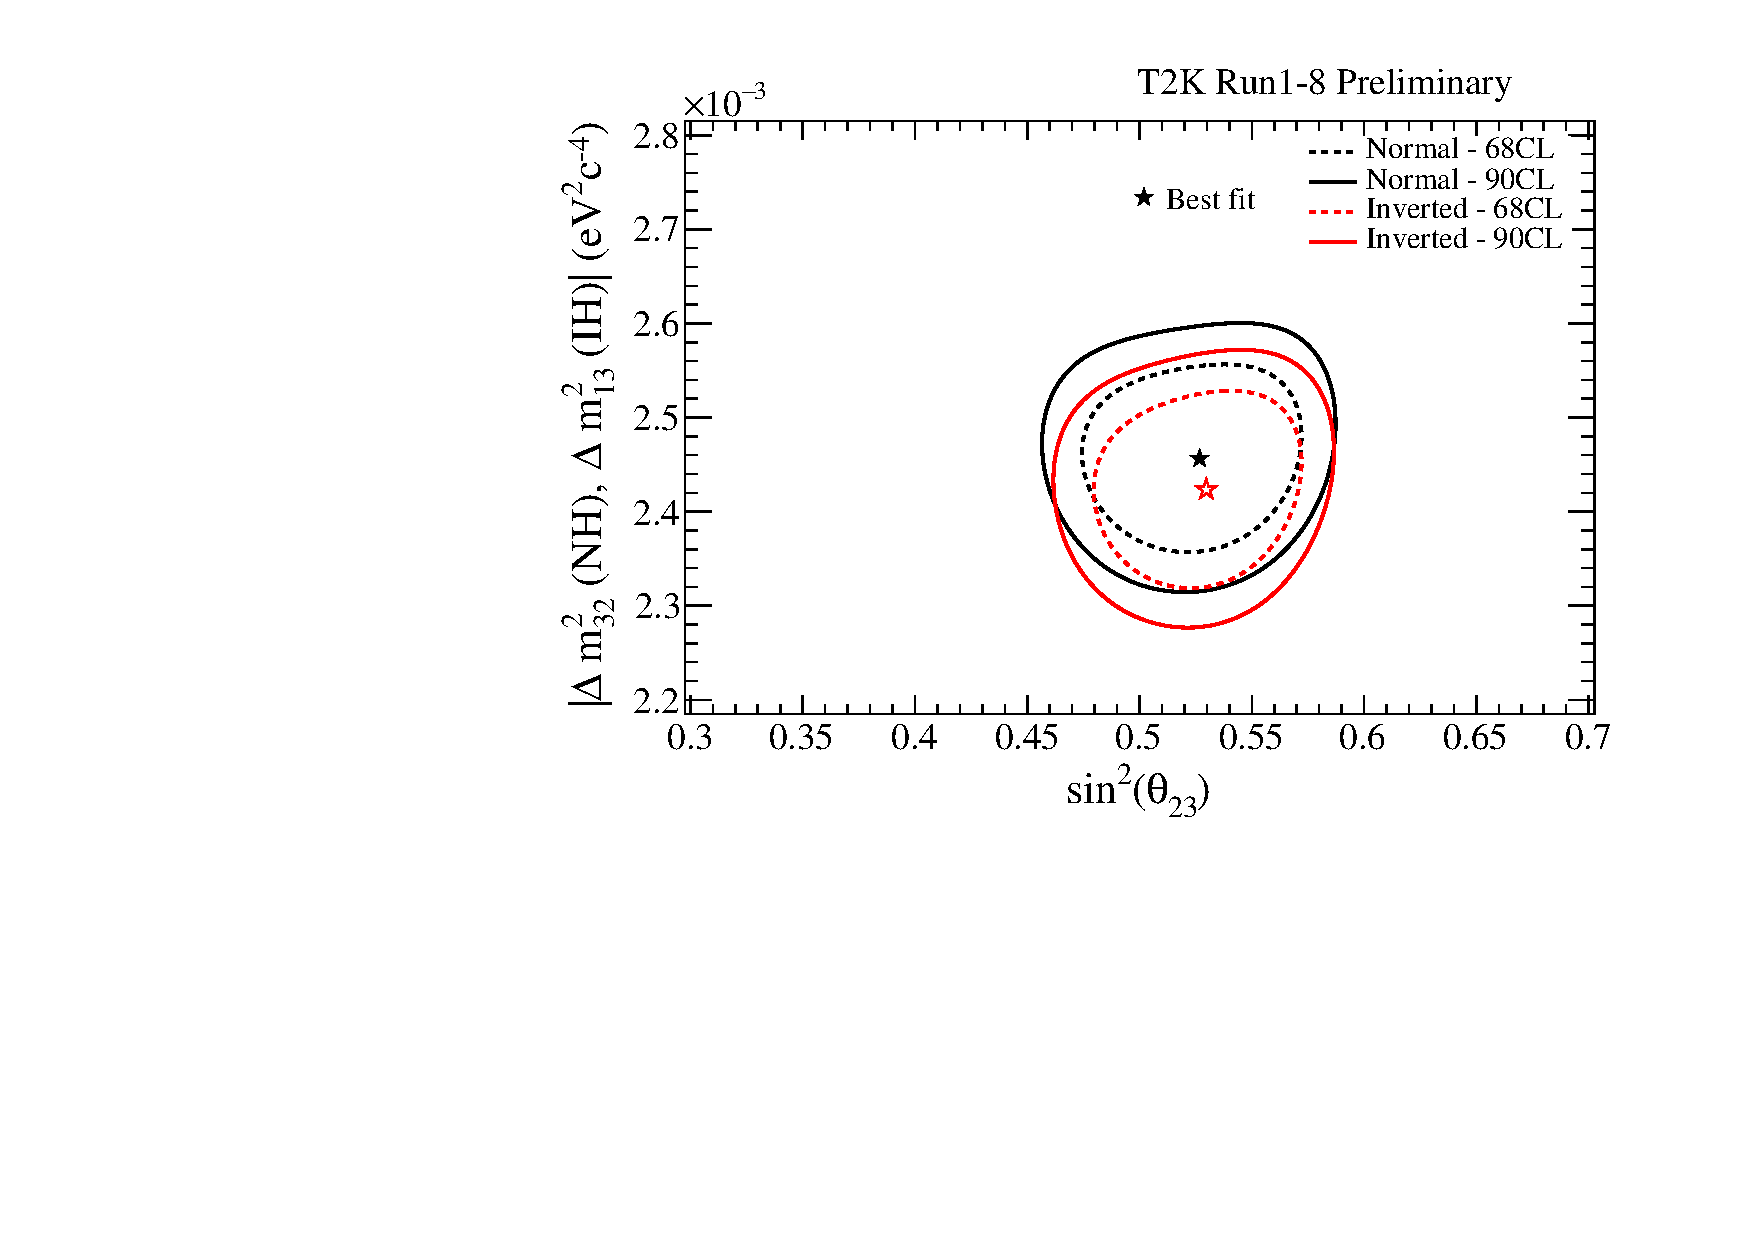
\includegraphics[width=0.9\textwidth]{data/reactor/2017b/mixing23_dmsq23_data_reactor_global}
		\caption{\disappearance with reactor constraint}
	\end{subfigure}
	\begin{subfigure}[b]{0.49\textwidth}
		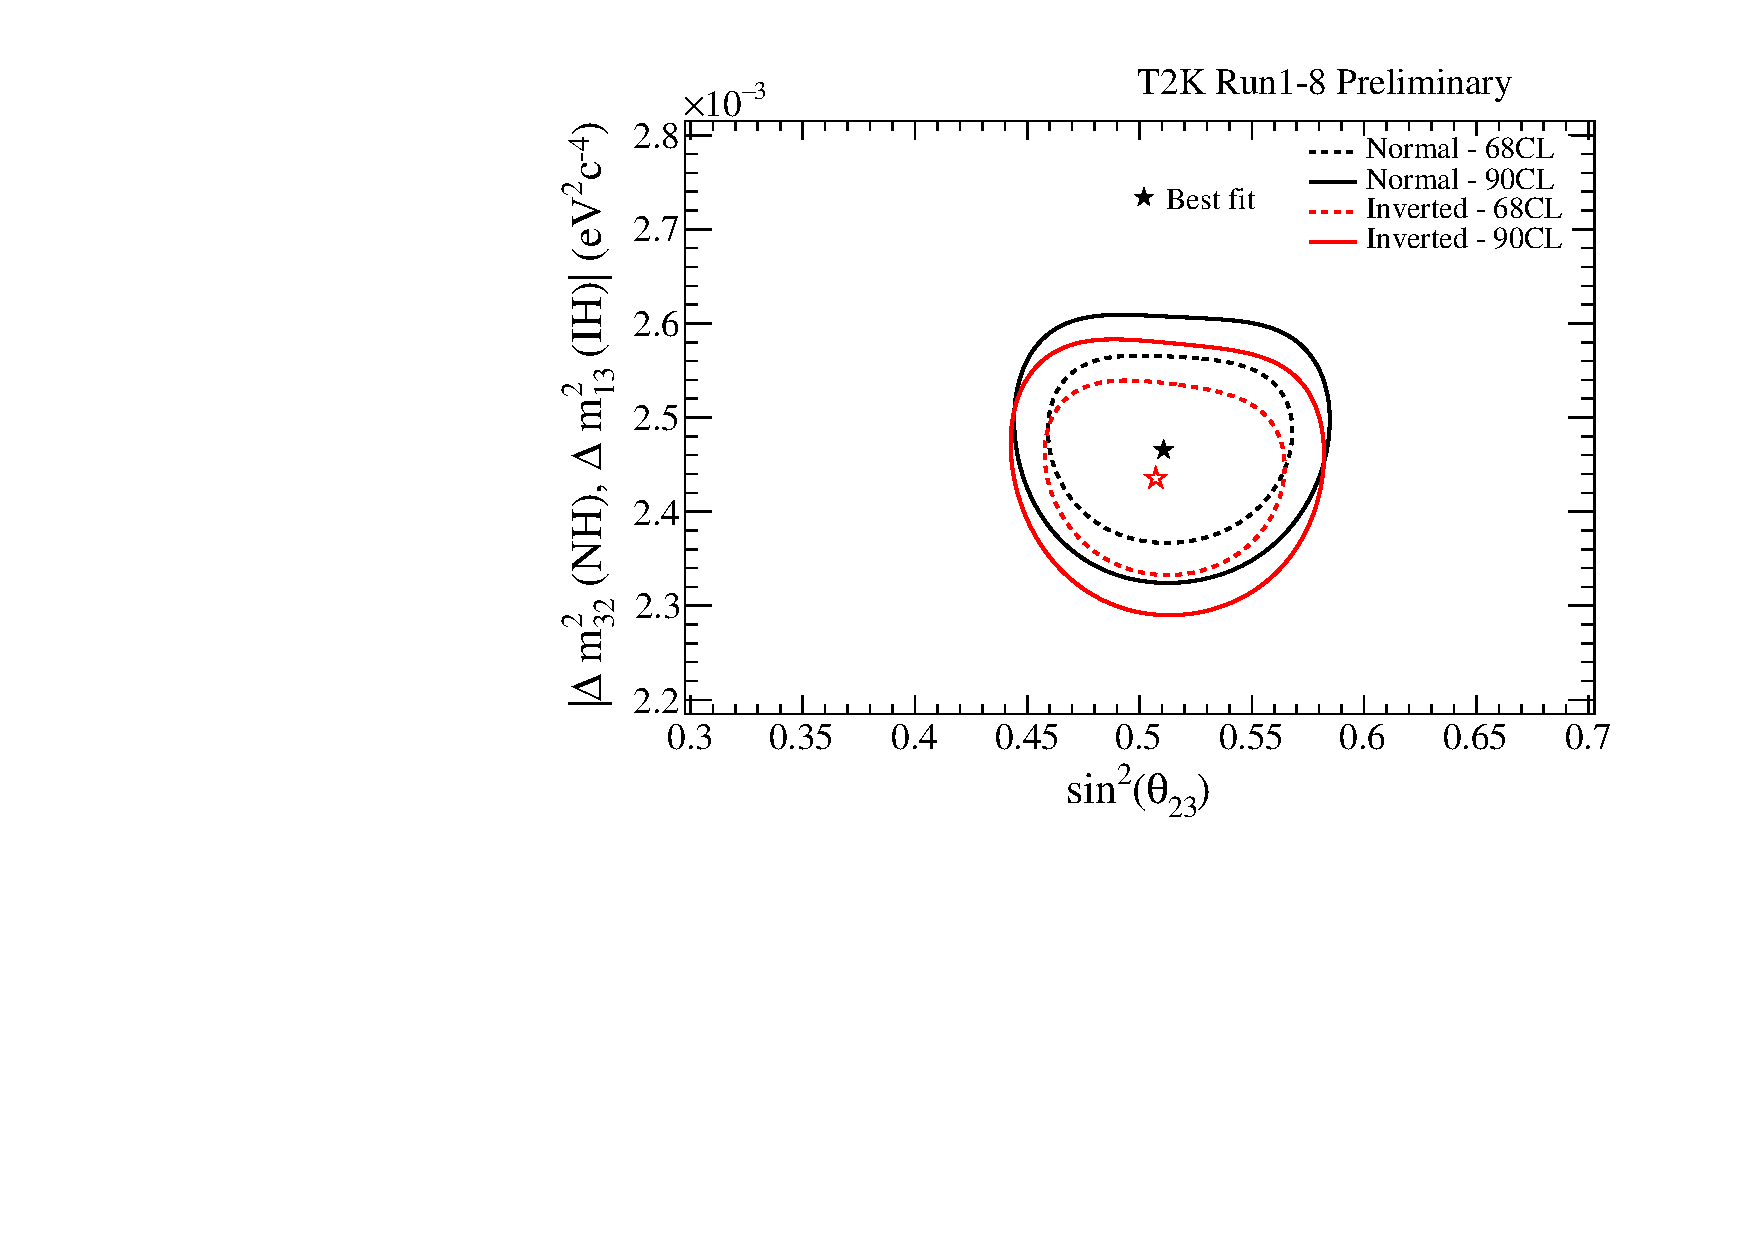
\includegraphics[width=0.9\textwidth]{data/t2k/2017b/mixing23_dmsq23_data_t2k_global}
		\caption{\disappearance T2K only}
	\end{subfigure}
	\caption {
		Contours at 68\% and 90\% CL for \disappearance with and without reactor constraint. Normal and inverted hierarchy contours are independent. All 5 samples were used to produce these fits.
	}
	\label{fig:ssqth23_vs_dmsq23_data_2017b}
\end{figure*}

\clearpage

\subsubsection{Results for \deltacp}

The result for \deltacp with reactor constraint and T2K only is shown in fig.~\ref{fig:dcp_data_2017b}.

\begin{figure*}[htb]
	\center
	\begin{subfigure}[b]{0.49\textwidth}
		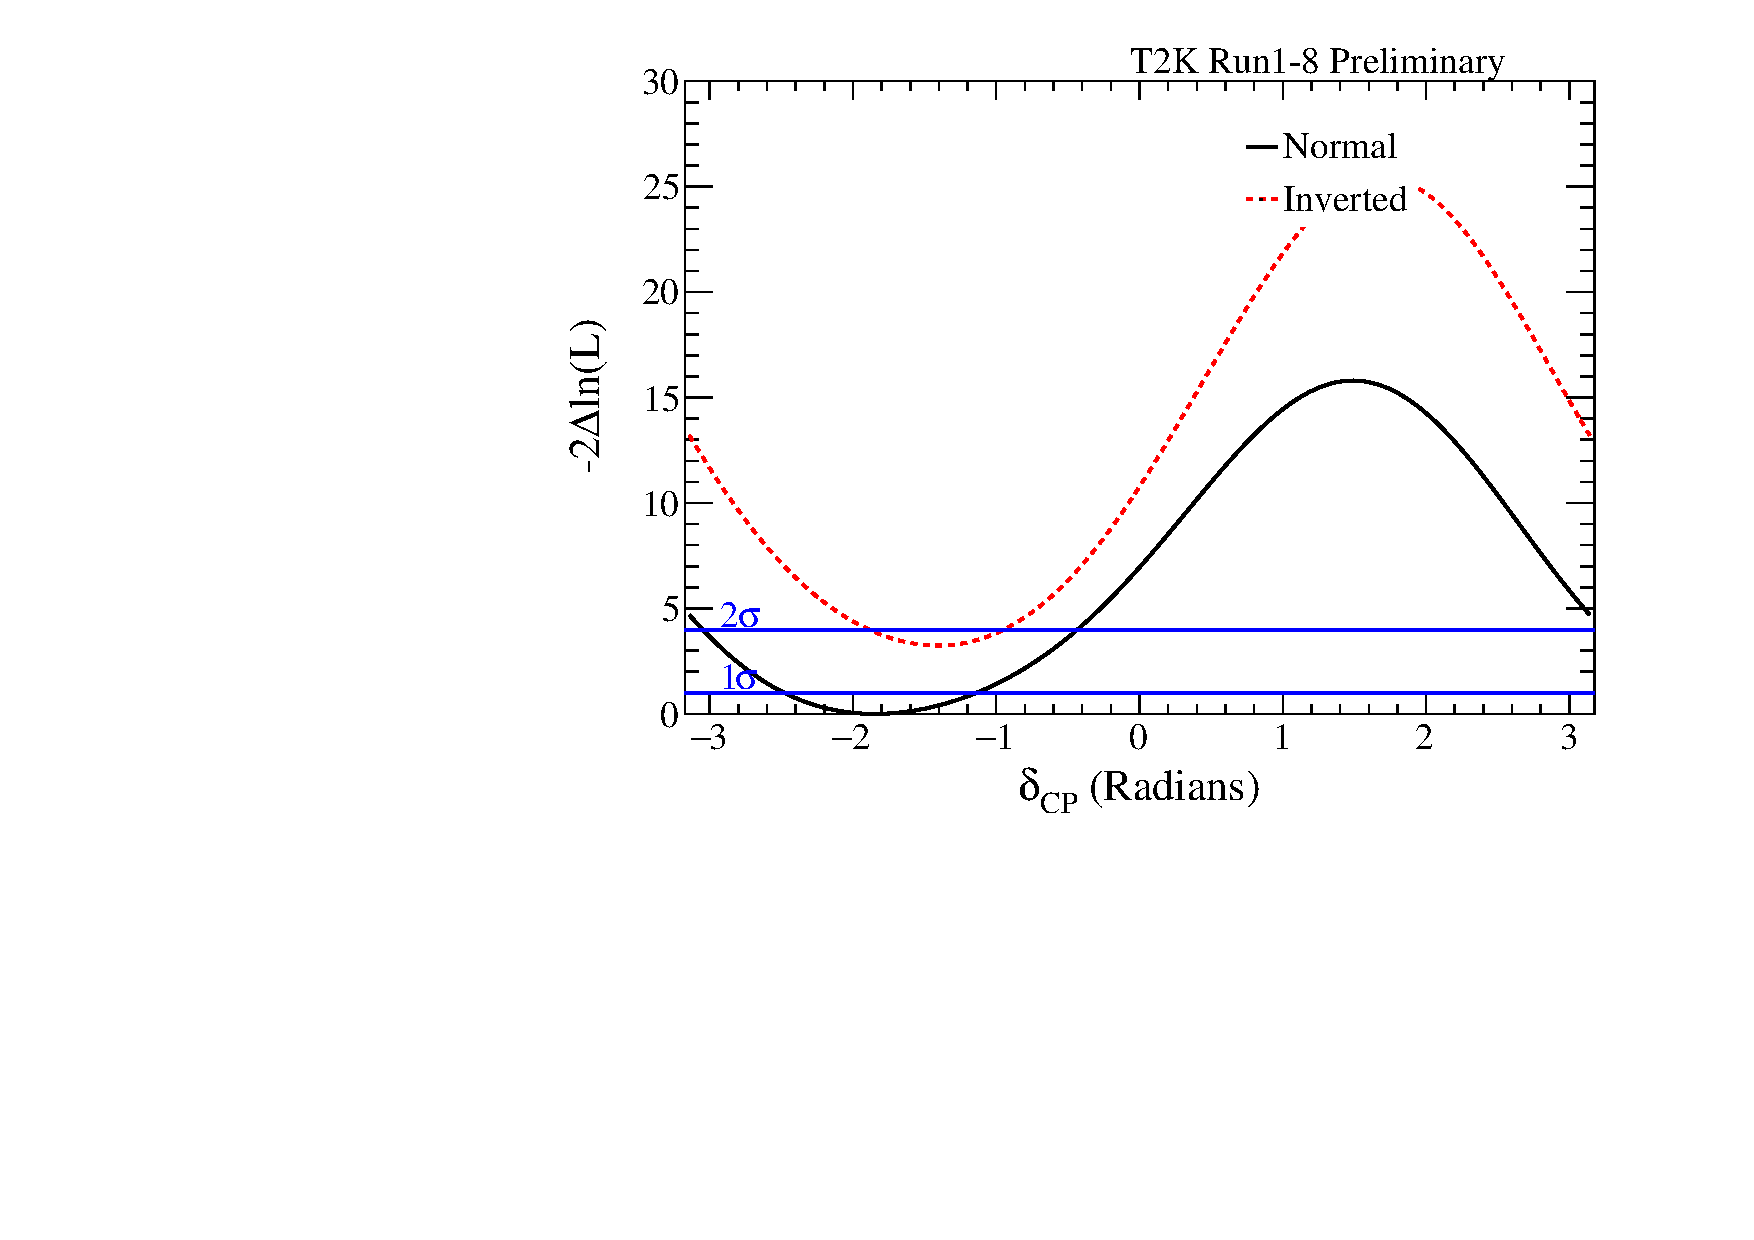
\includegraphics[width=0.9\textwidth]{data/reactor/2017b/deltacp_data_reactor_global}
		\caption{\deltacp with reactor constraint}
	\end{subfigure}
	\begin{subfigure}[b]{0.49\textwidth}
		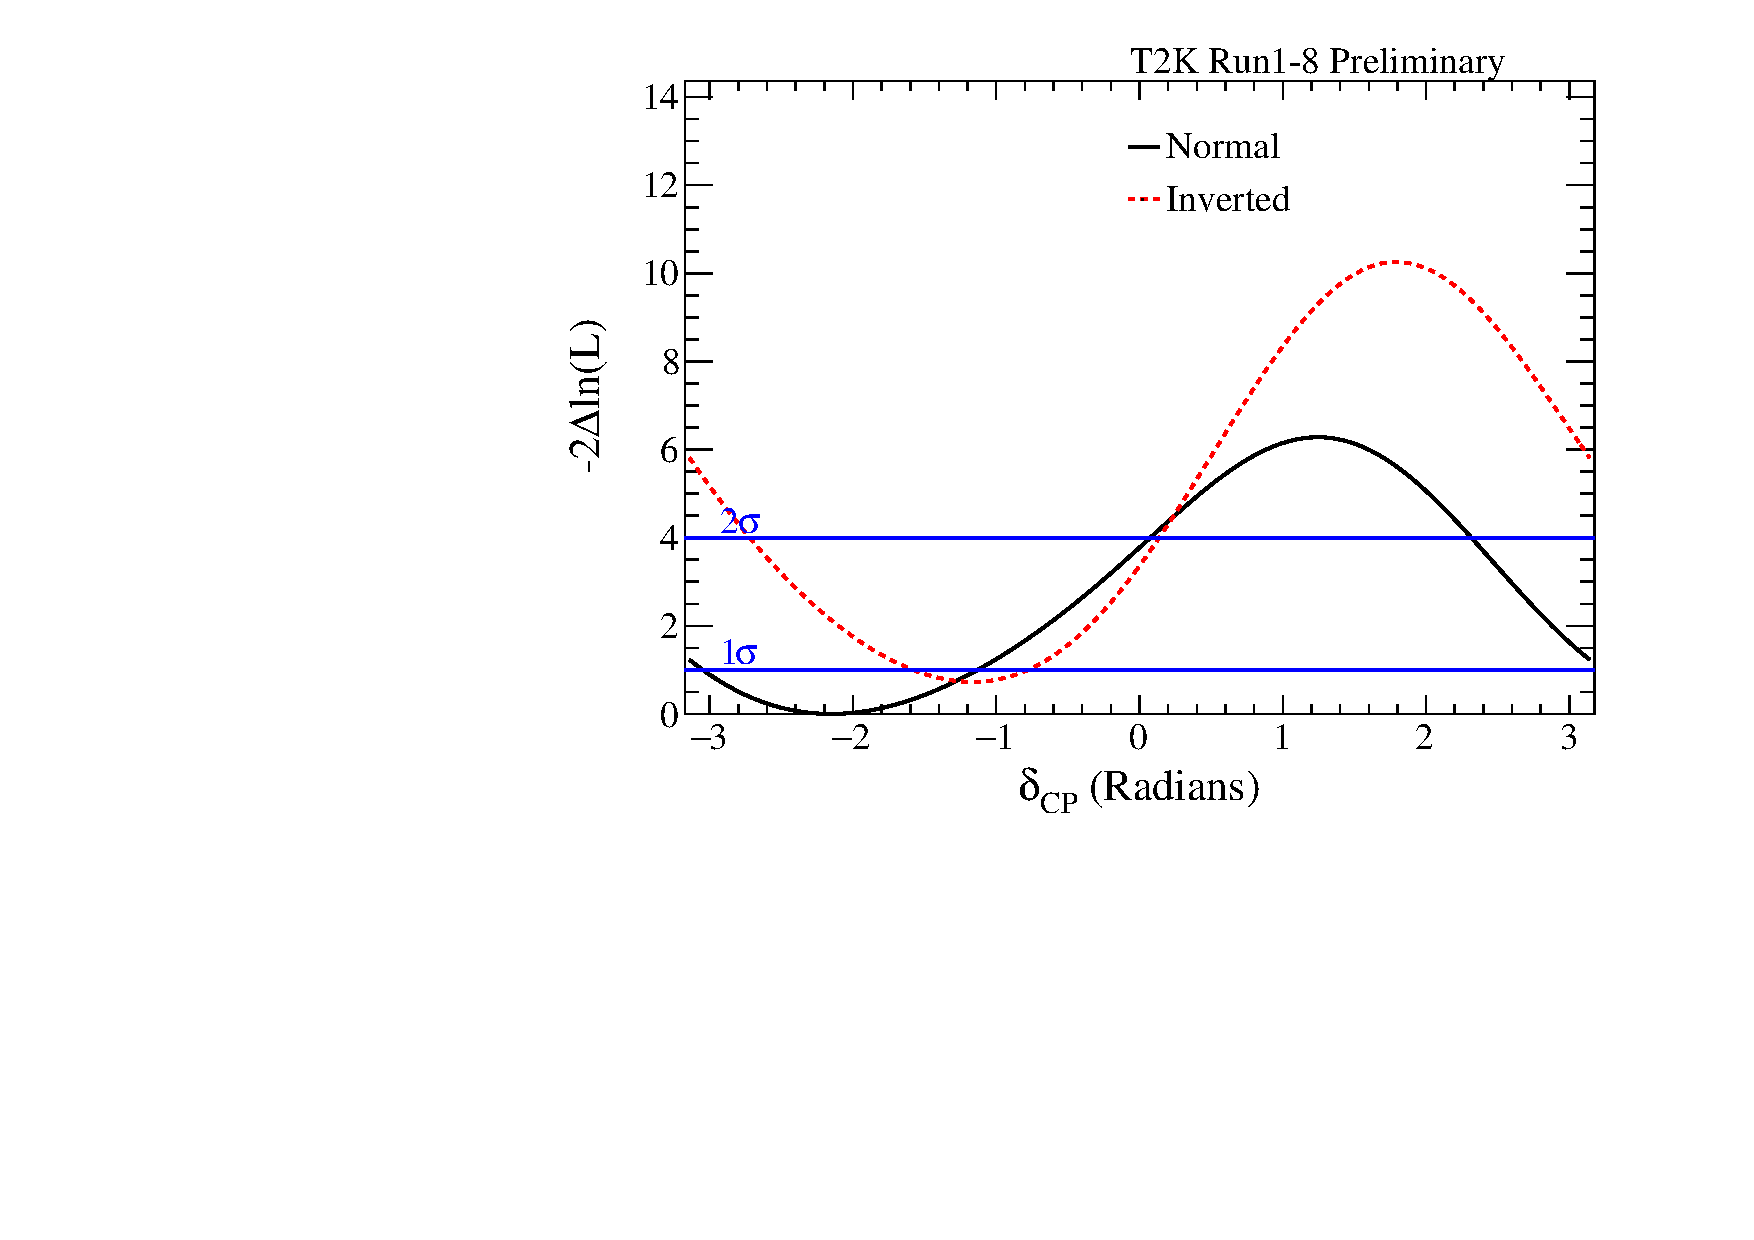
\includegraphics[width=0.9\textwidth]{data/t2k/2017b/deltacp_data_t2k_global}
		\caption{\deltacp T2K only}
	\end{subfigure}
	\caption {
		The expected $\Delta\chi^2$ distribution as a function of \deltacp with and without reactor constraint. The mass hierarchy is minimized, with normal and inverted hierarchy $\Delta\chi^2$ distributions shifted to the same global best-fit $\chi^2$ value, which is taken to be the minimum between normal and inverted hierarchy. All 5 samples were used to produce these fits.
	}
	\label{fig:dcp_data_2017b}
\end{figure*}

\subsubsection{Results for \ssqthonethree}

The result for \ssqthonethree (without reactor constraint) is shown in fig.~\ref{fig:th13_data_2017b}.

\begin{figure*}[htb]
	\center
	\begin{subfigure}[b]{0.49\textwidth}
		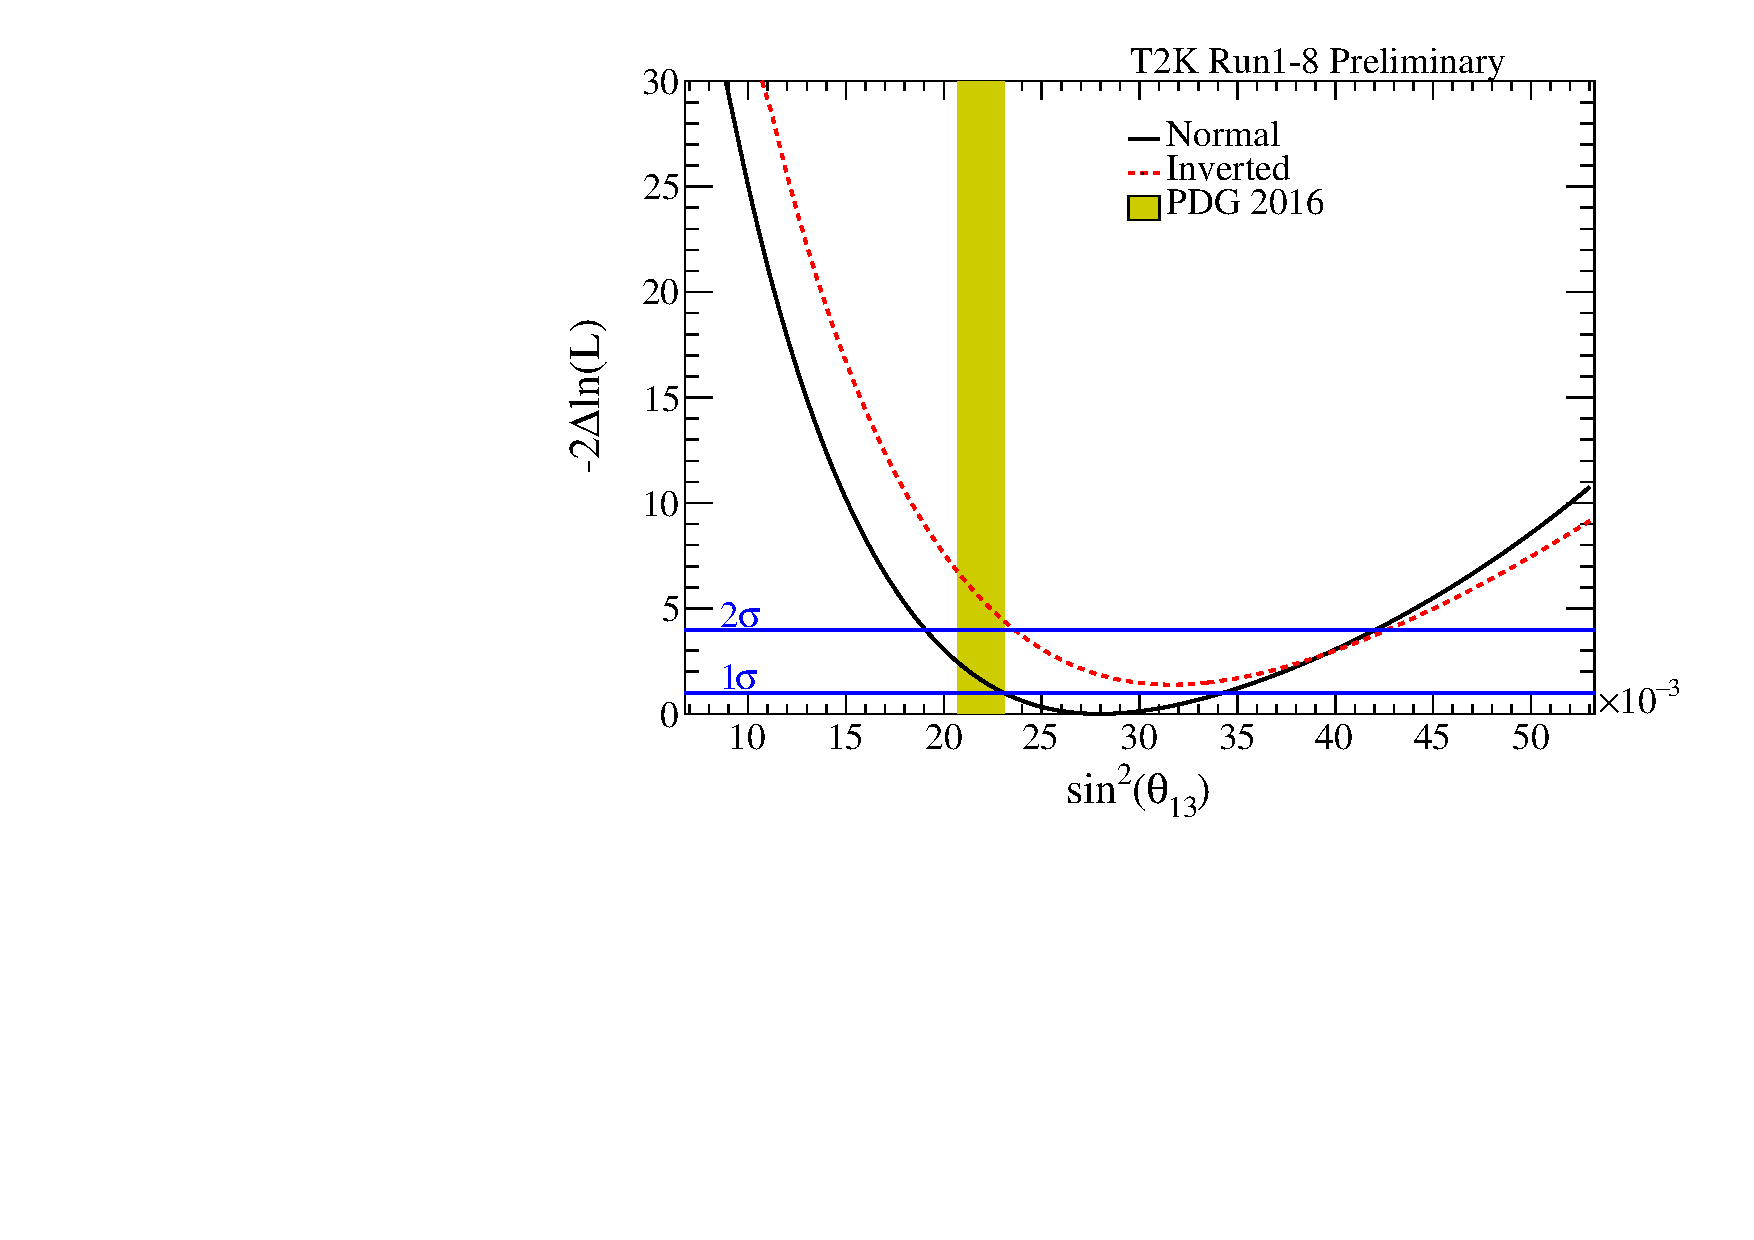
\includegraphics[width=0.9\textwidth]{data/t2k/2017b/mixing13_data_t2k_global}
		\caption{\ssqthonethree T2K only}
	\end{subfigure}
	\caption {
		The expected $\Delta\chi^2$ distribution as a function of \ssqthonethree without reactor constraint. The mass hierarchy is minimized, with normal and inverted hierarchy $\Delta\chi^2$ distributions shifted to the same global best-fit $\chi^2$ value, which is taken to be the minimum between normal and inverted hierarchy. All 5 samples were used to produce these fits.
	}
	\label{fig:th13_data_2017b}
\end{figure*}

\clearpage

\subsubsection{Results for \ssqthtwothree}

The result for \ssqthtwothree with reactor constraint and T2K only is shown in fig.~\ref{fig:th23_data_2017b}.

\begin{figure*}[htb]
	\center
	\begin{subfigure}[b]{0.49\textwidth}
		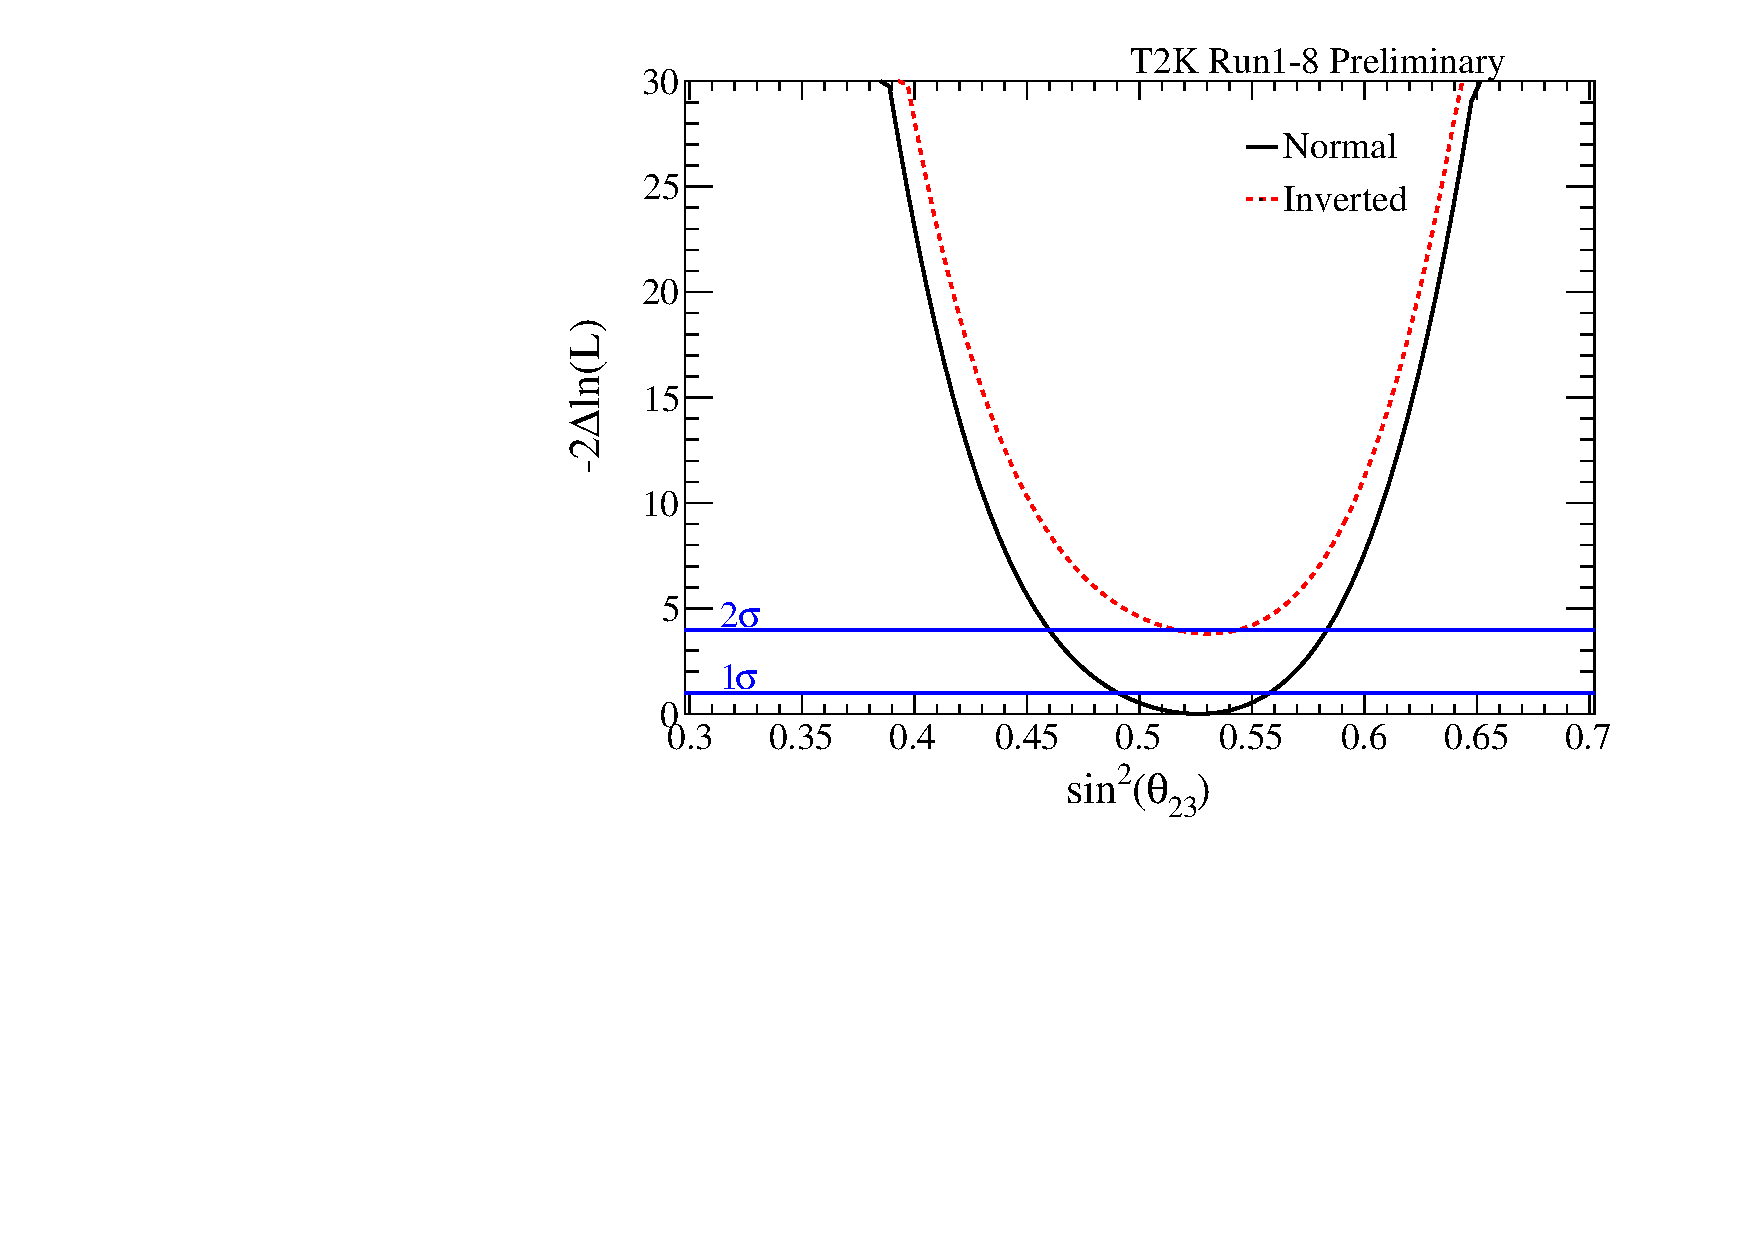
\includegraphics[width=0.9\textwidth]{data/reactor/2017b/mixing23_data_reactor_global}
		\caption{\ssqthtwothree with reactor constraint}
	\end{subfigure}
	\begin{subfigure}[b]{0.49\textwidth}
		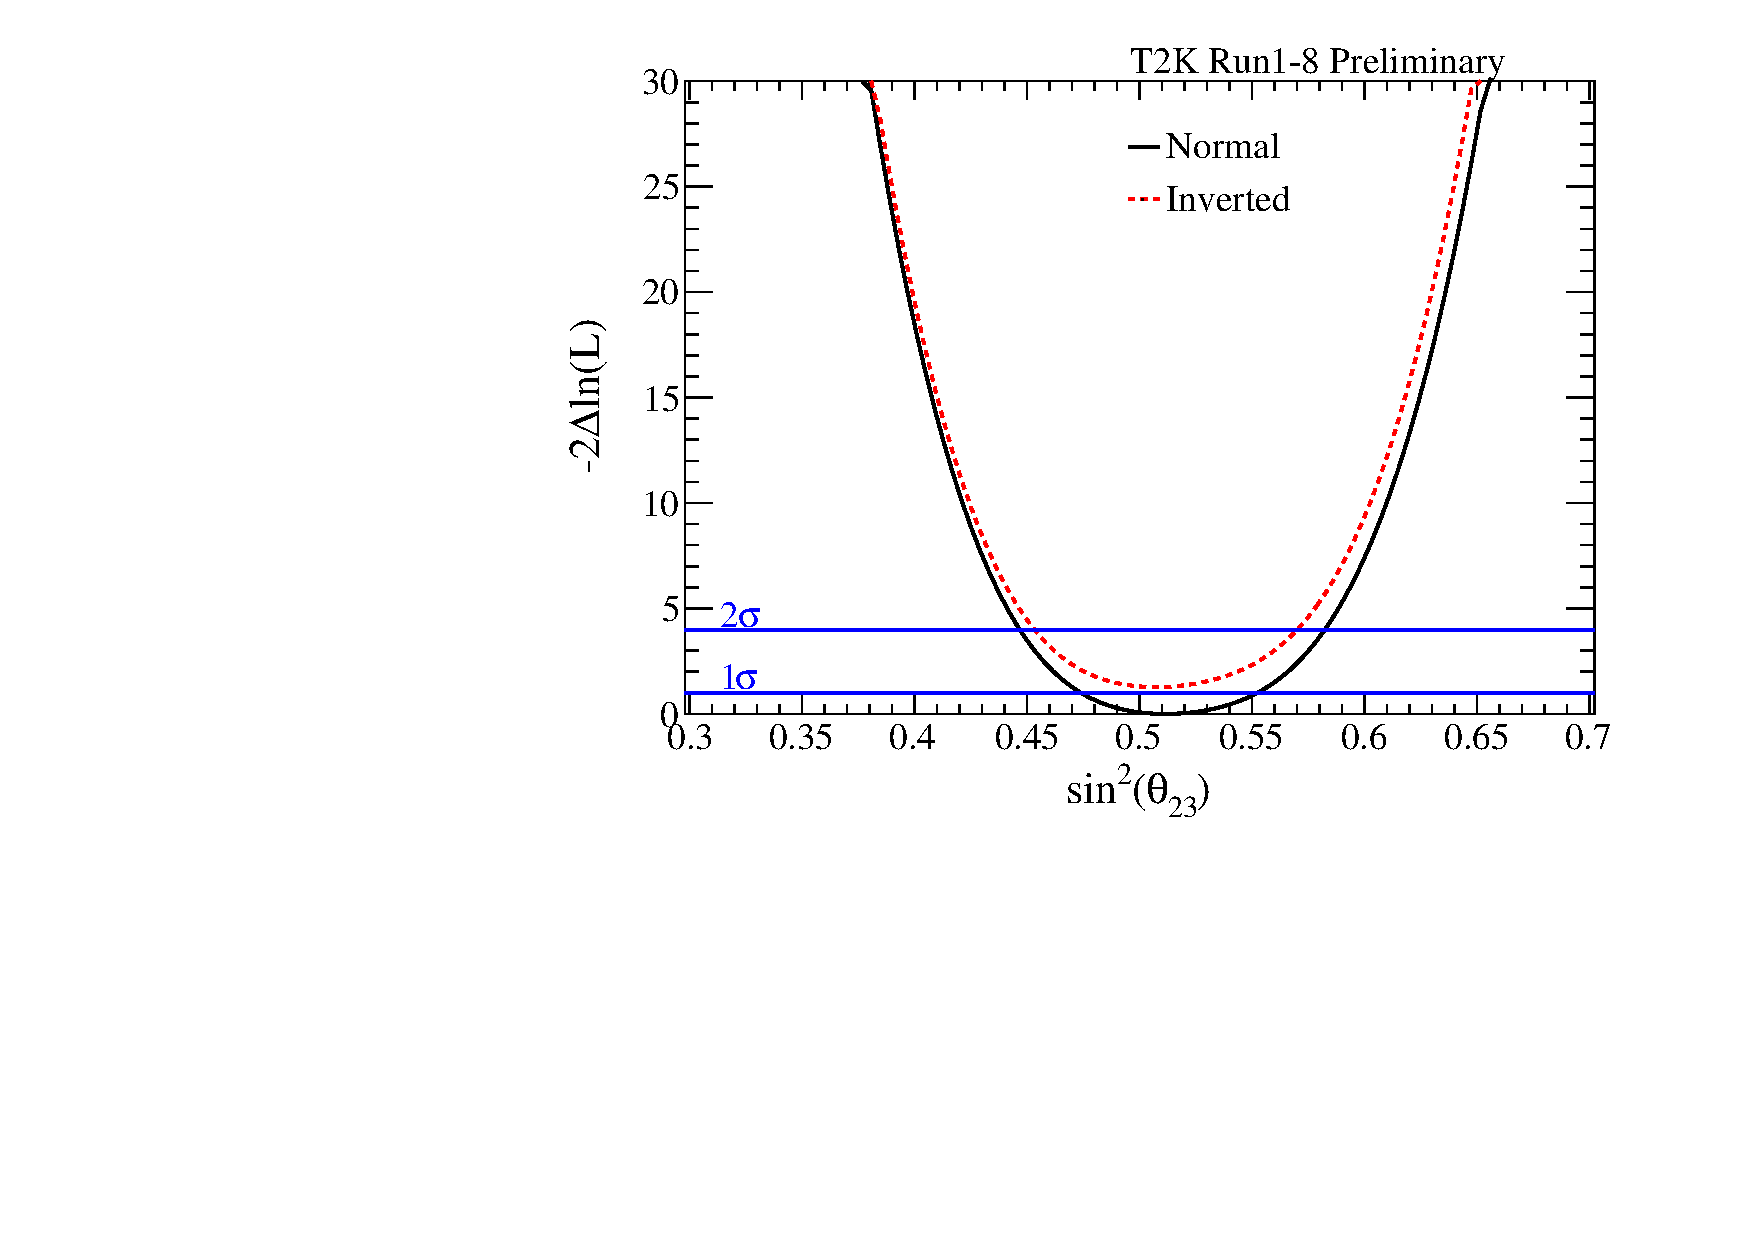
\includegraphics[width=0.9\textwidth]{data/t2k/2017b/mixing23_data_t2k_global}
		\caption{\ssqthtwothree T2K only}
	\end{subfigure}
	\caption {
		The expected $\Delta\chi^2$ distribution as a function of \ssqthtwothree with and without reactor constraint. The mass hierarchy is minimized, with normal and inverted hierarchy $\Delta\chi^2$ distributions shifted to the same global best-fit $\chi^2$ value, which is taken to be the minimum between normal and inverted hierarchy. All 5 samples were used to produce these fits.
	}
	\label{fig:th23_data_2017b}
\end{figure*}

\subsubsection{Results for \dmsq}

The result for \dmsq with reactor constraint and T2K only is shown in fig.~\ref{fig:dmsq23_data_2017b}.

\begin{figure*}[htb]
	\center
	\begin{subfigure}[b]{0.49\textwidth}
		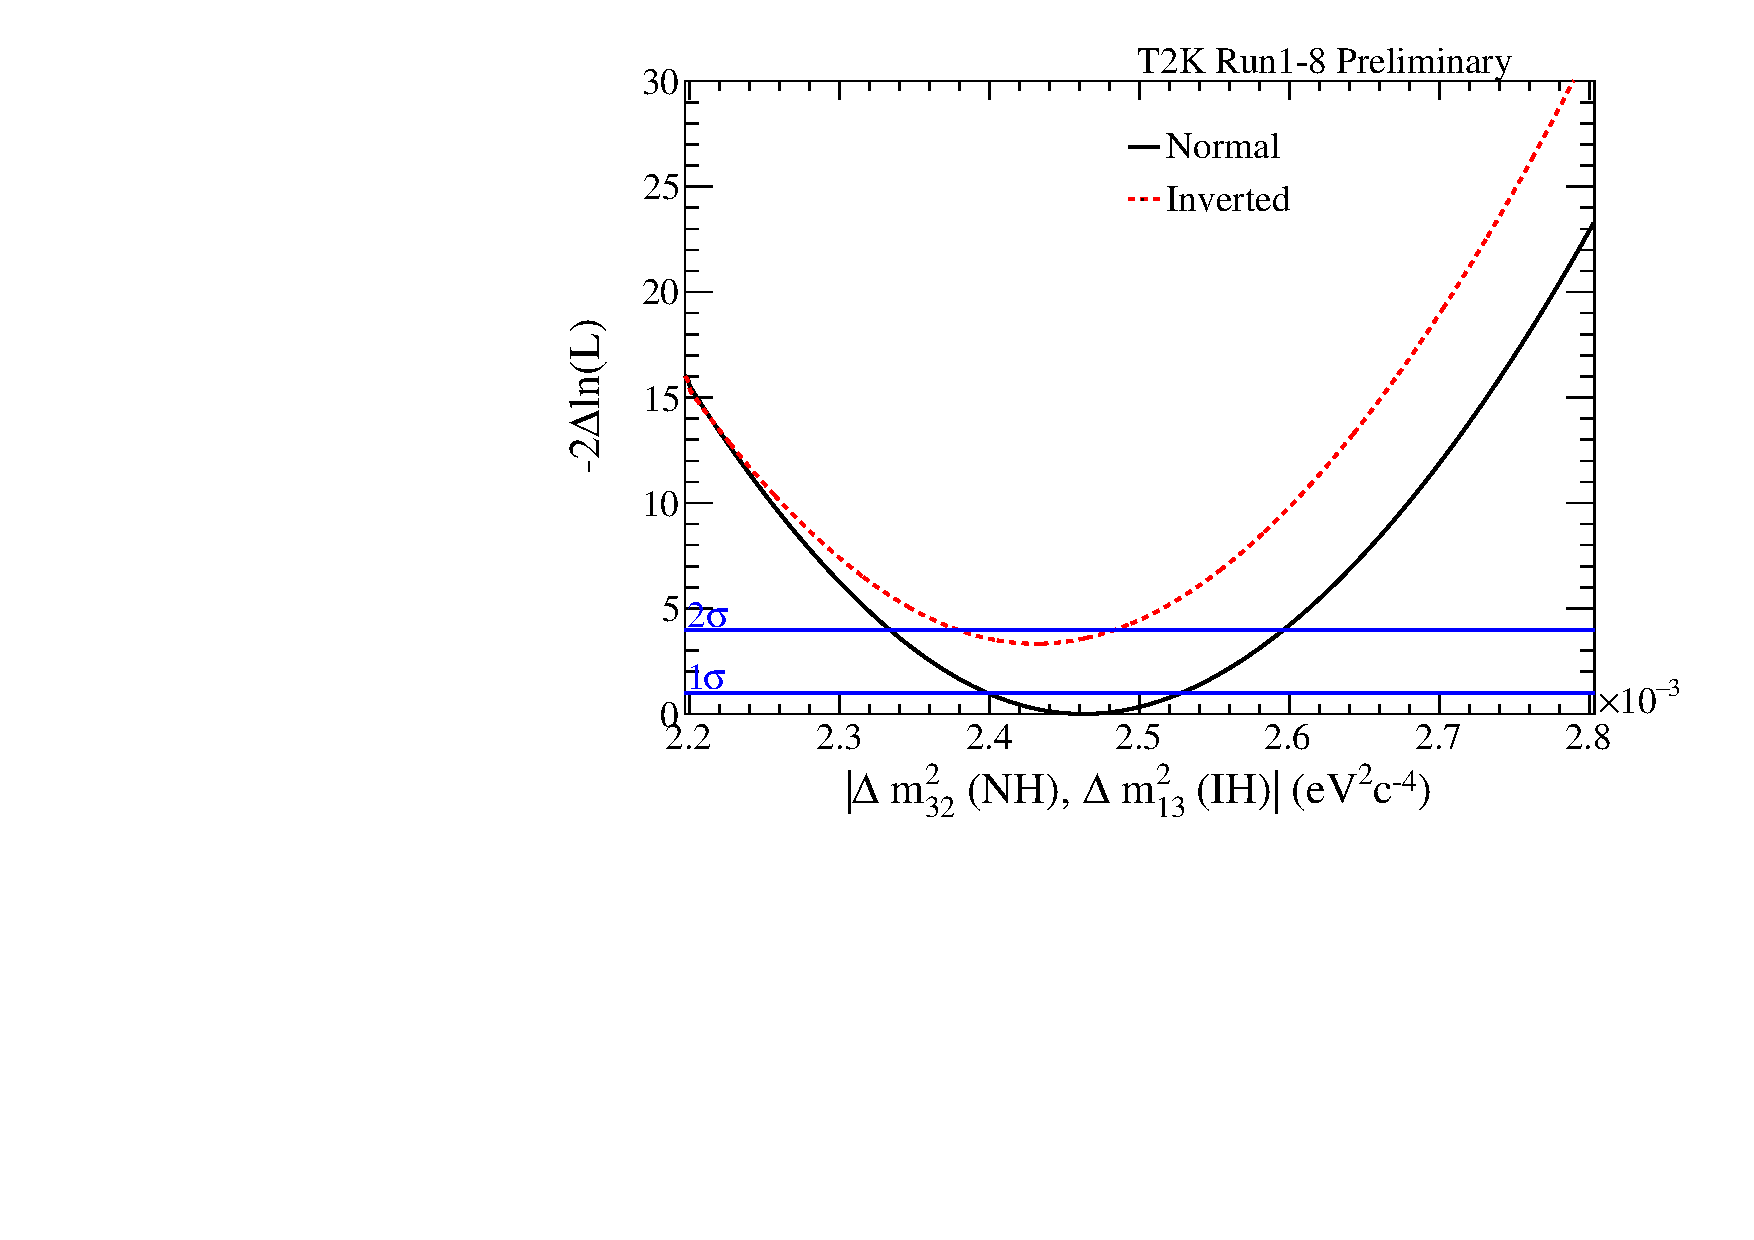
\includegraphics[width=0.9\textwidth]{data/reactor/2017b/dmsq23_data_reactor_global}
		\caption{\dmsq with reactor constraint}
	\end{subfigure}
	\begin{subfigure}[b]{0.49\textwidth}
		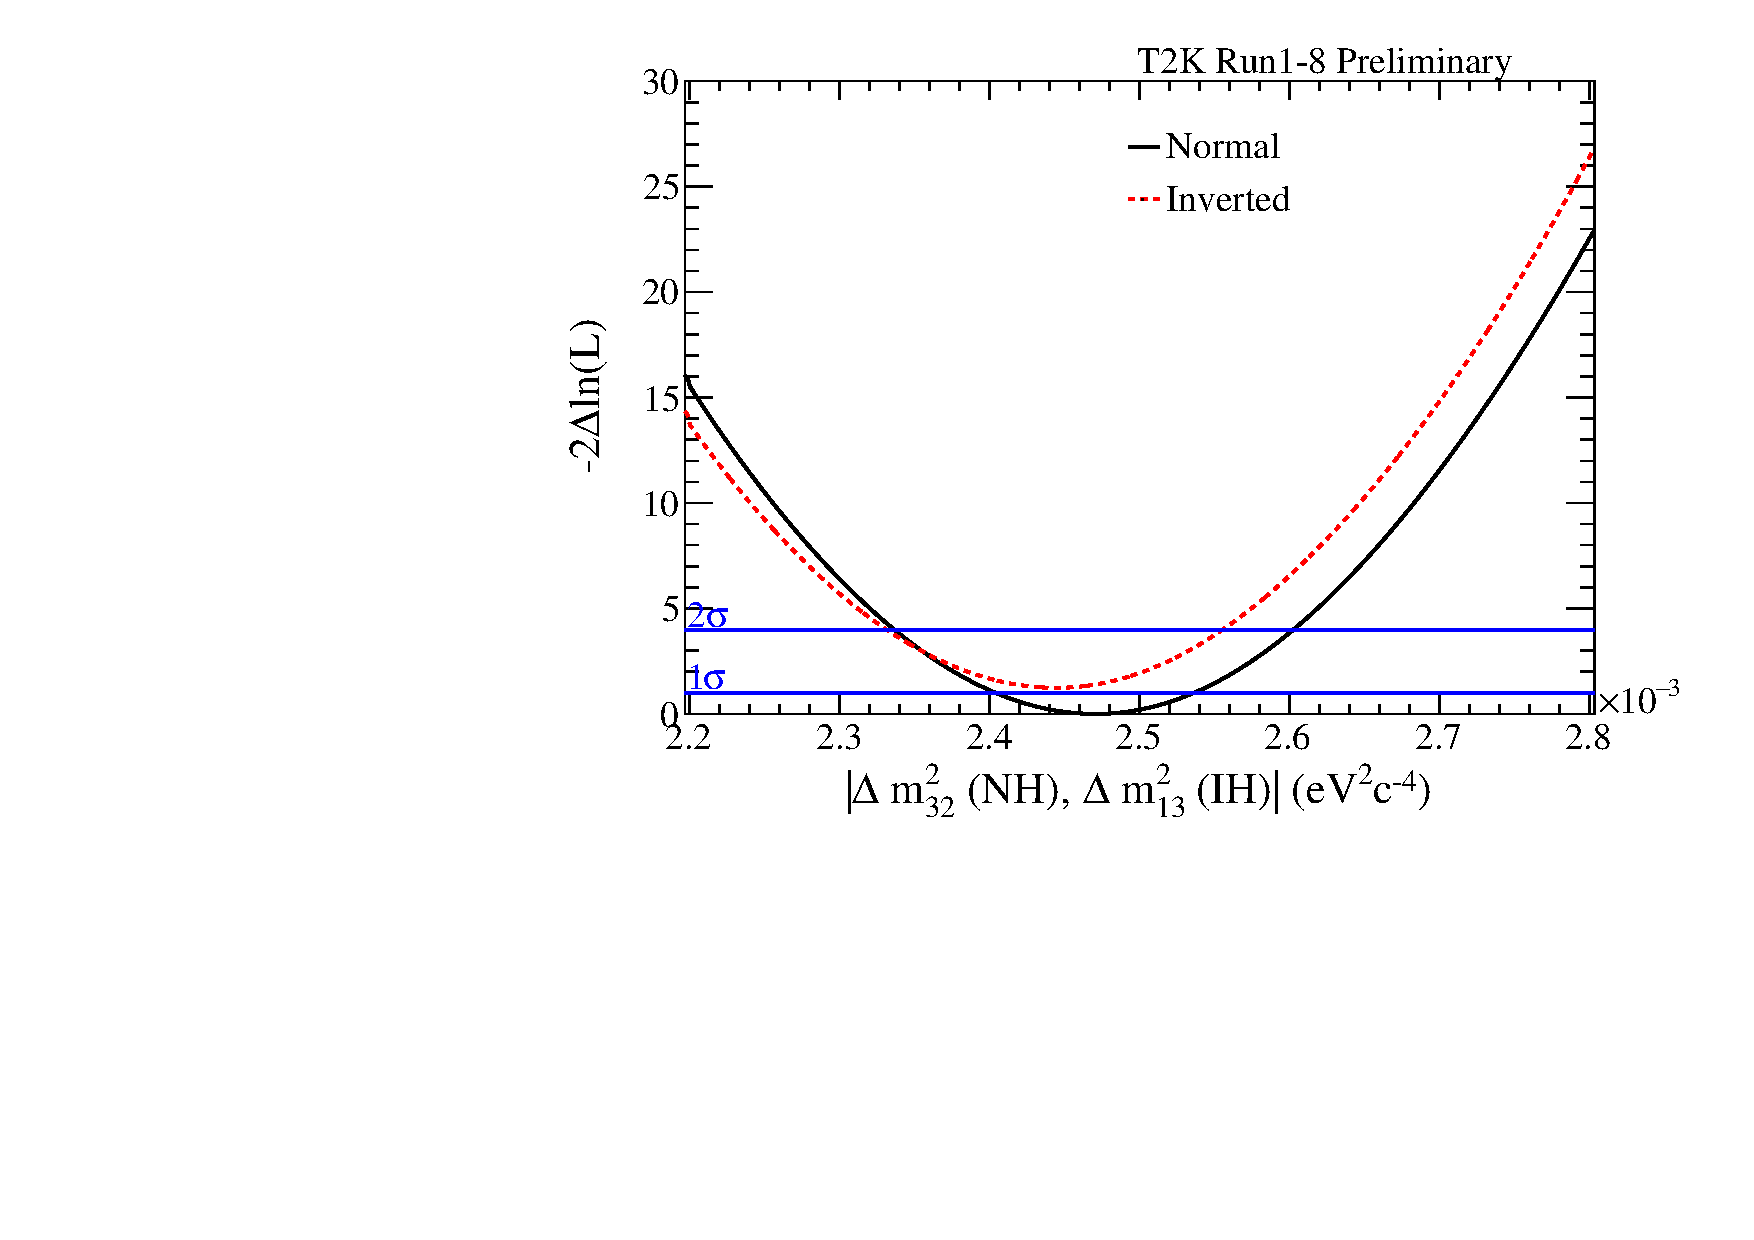
\includegraphics[width=0.9\textwidth]{data/t2k/2017b/dmsq23_data_t2k_global}
		\caption{\dmsq T2K only}
	\end{subfigure}
	\caption {
		The expected $\Delta\chi^2$ distribution as a function of \dmsq with and without reactor constraint. The mass hierarchy is minimized, with normal and inverted hierarchy $\Delta\chi^2$ distributions shifted to the same global best-fit $\chi^2$ value, which is taken to be the minimum between normal and inverted hierarchy. All 5 samples were used to produce these fits.
	}
	\label{fig:dmsq23_data_2017b}
\end{figure*}

\subsection {Feldman-Cousins simultaneous fit of \deltacp and mass hierarchy}
\label{sec:fc_significance_2017b}

This section presents the results of the Feldman-Cousins fit of \deltacp and mass hierarchy. Throws of oscillation parameters are made according to PDG 2016 best-fit values and errors for \ssqthonethree, \ssqthonetwo and \dmsqonetwo, whilst \ssqthtwothree and \dmsq are thrown according to the smeared likelihood distribution produced by an Asimov fit using the best-fit from data for these parameters. \deltacp is fixed at one of 9 evenly specified values on the range $\left[-\pi,\pi\right]$.

\subsubsection{Input oscillation parameters}
\label{sec:fc_significance:inputs_2017b}

The distributions of oscillation parameters (for normal hierarchy) are shown in \cref{fig:fc_input_dist_2017b}. The distributions of the atmospheric parameters are shown in \cref{fig:fc_input_disapp_2017b}.

\begin{figure*}[htb]
	\center
	\begin{subfigure}[b]{0.49\textwidth}
		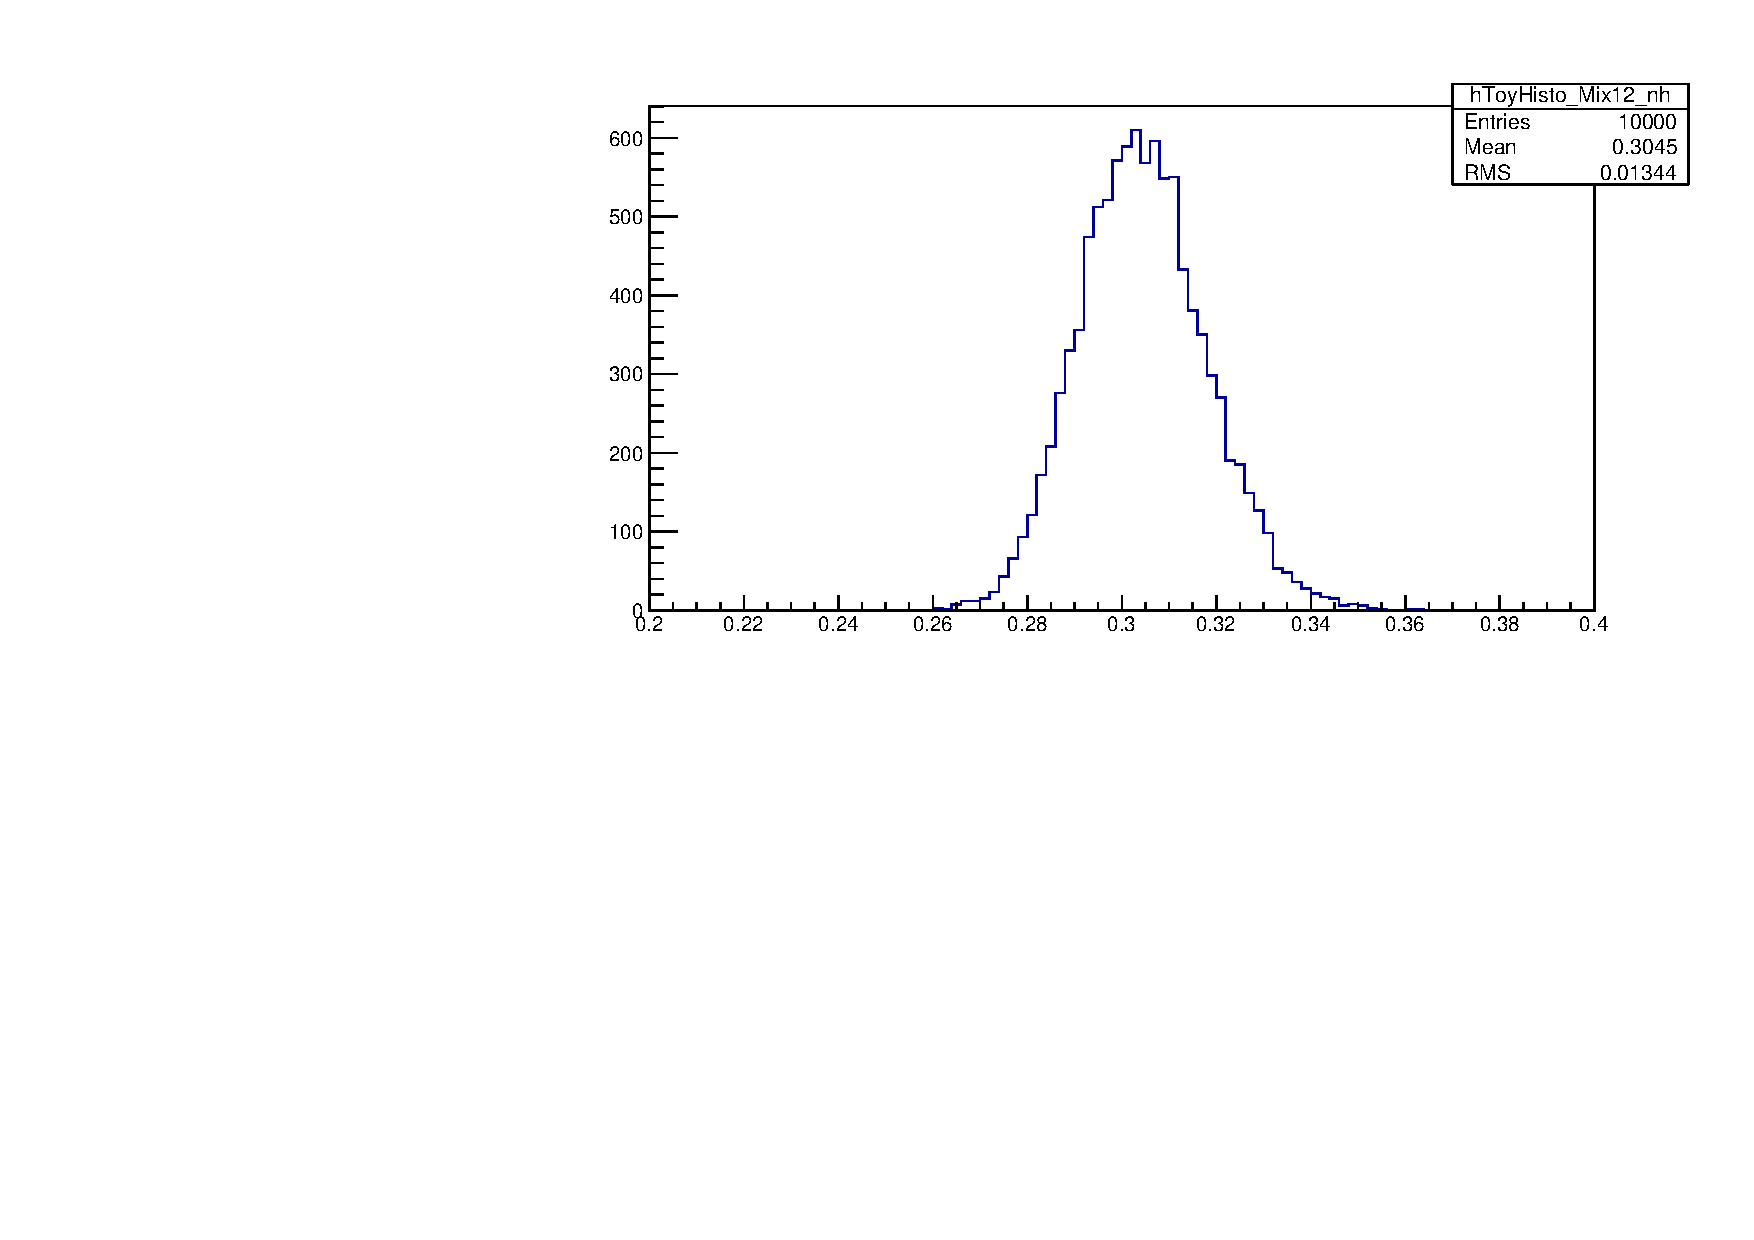
\includegraphics[width=0.9\textwidth]{data/fc/inputs/2017b/mixing12_in}
		\caption{\ssqthonetwo}
	\end{subfigure}
	\begin{subfigure}[b]{0.49\textwidth}
		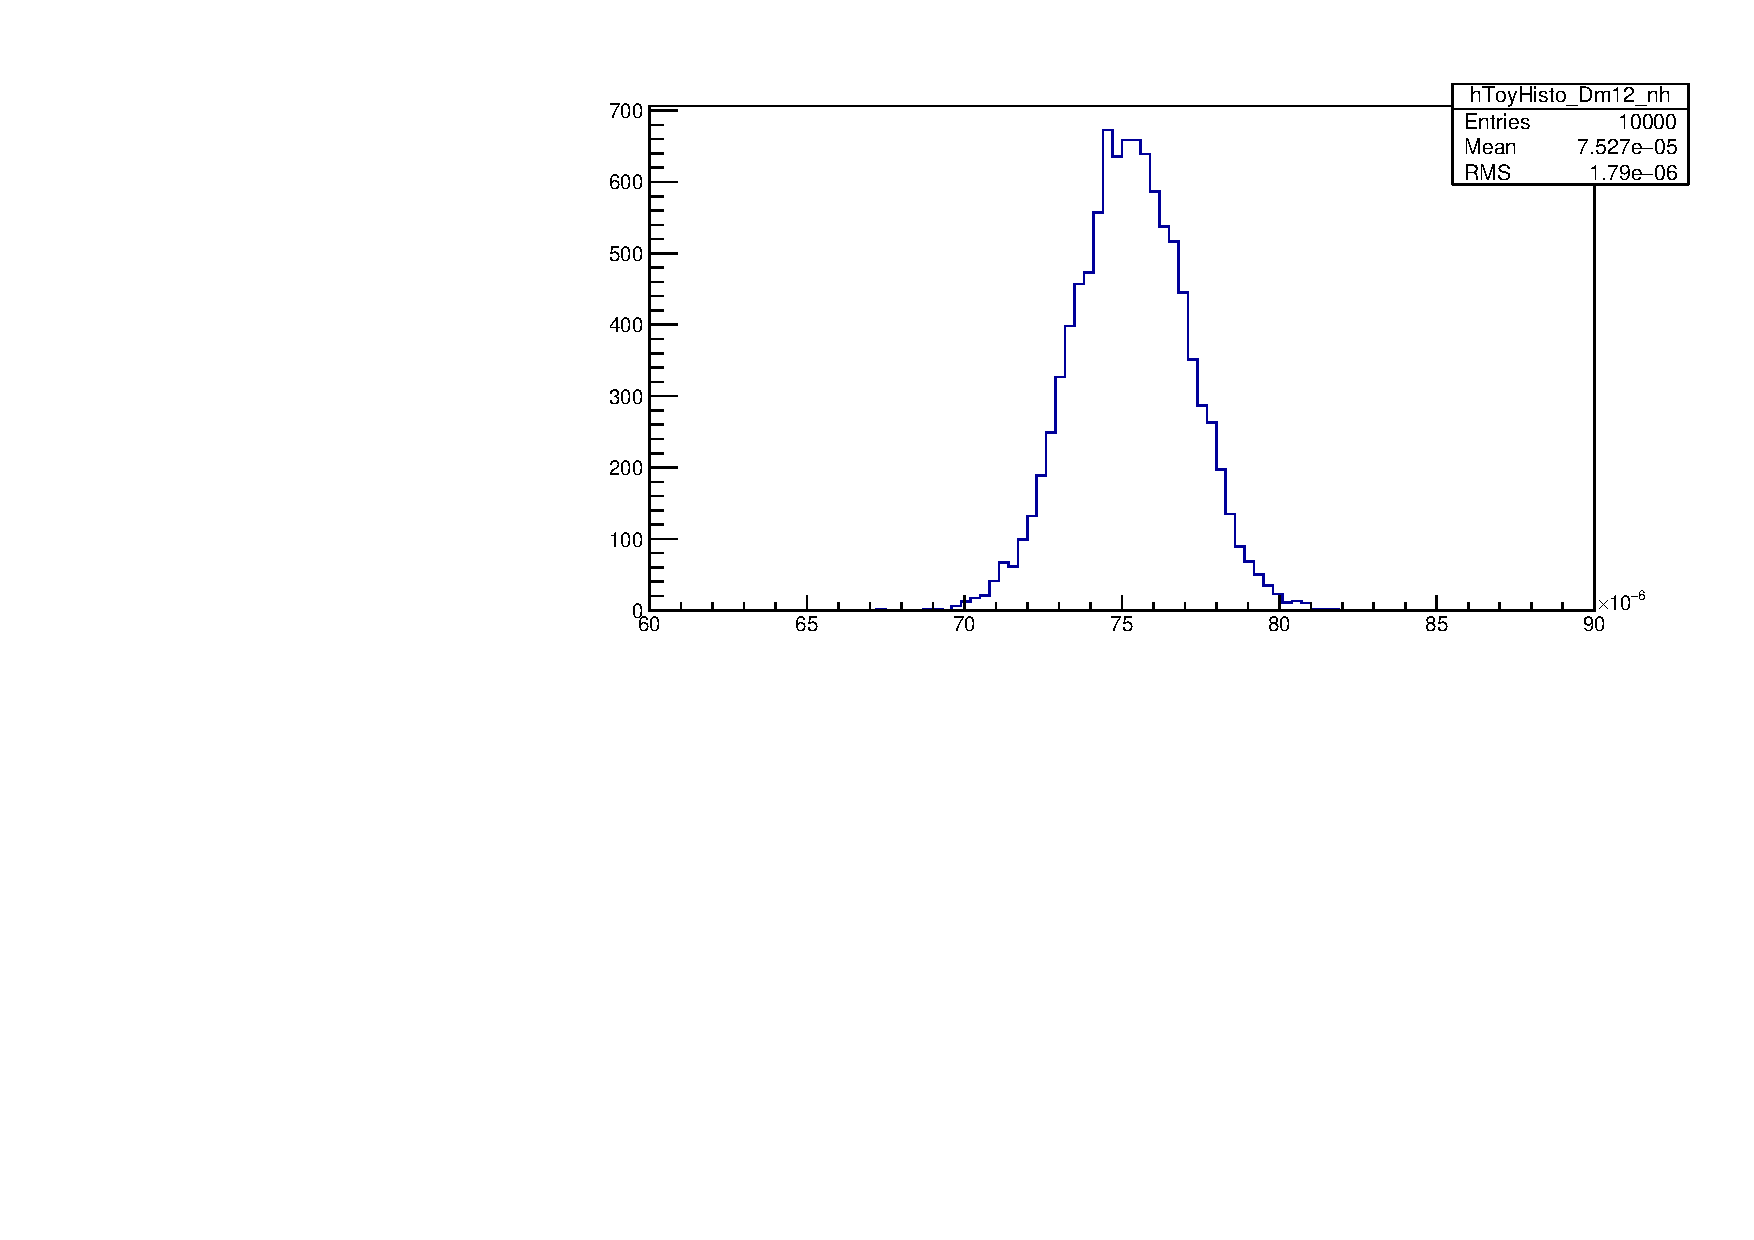
\includegraphics[width=0.9\textwidth]{data/fc/inputs/2017b/dmsq12_in}
		\caption{\dmsqonetwo}
	\end{subfigure}
	\begin{subfigure}[b]{0.49\textwidth}
		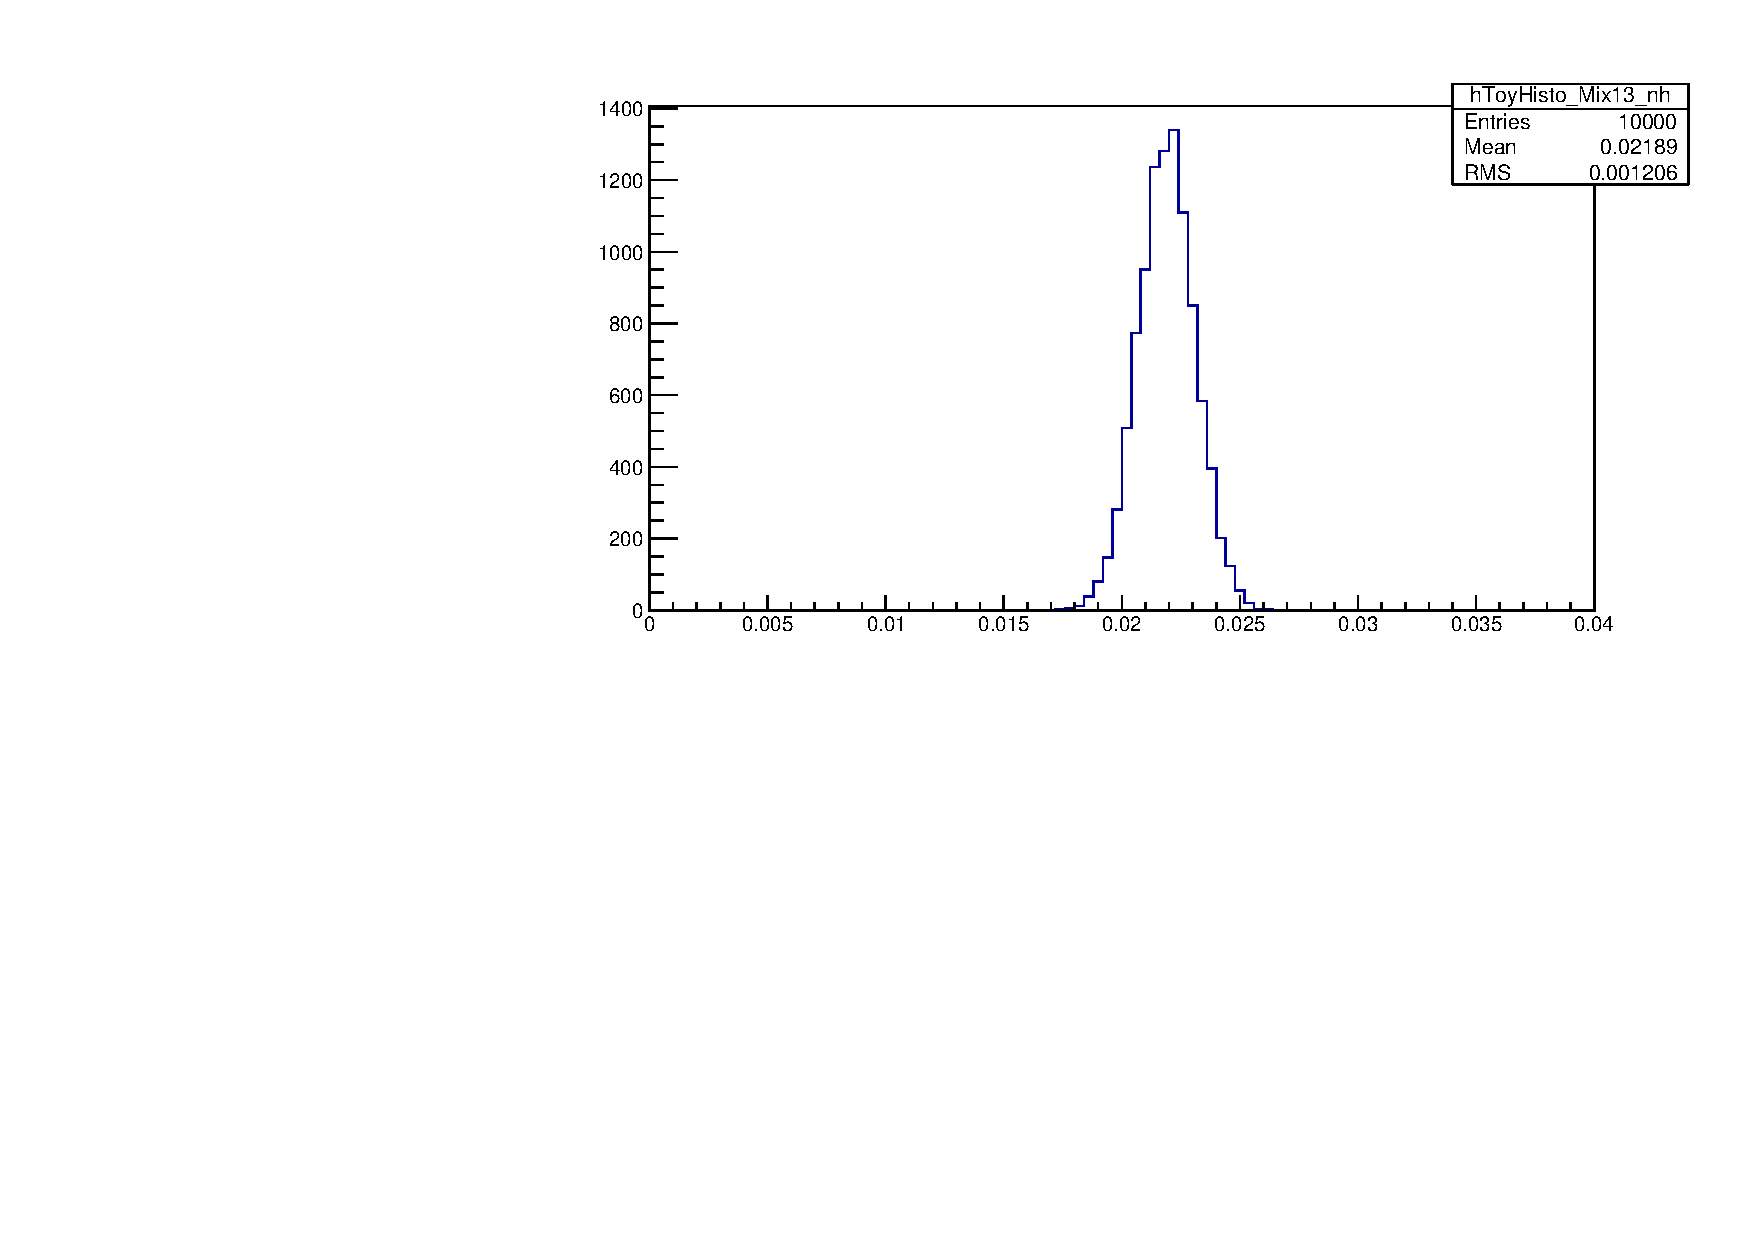
\includegraphics[width=0.9\textwidth]{data/fc/inputs/2017b/mixing13_in}
		\caption{\ssqthonethree}
	\end{subfigure}
	\caption {
		Distribution of oscillation parameter throws for Feldman-Cousins fits.
	}
	\label{fig:fc_input_dist_2017b}
\end{figure*}

\begin{figure*}[htb]
	\begin{subfigure}[b]{0.49\textwidth}
		\includegraphics[width=0.9\textwidth, page=2]{data/fc/inputs/2017b/disappearance_nh_likelihood}
		\caption{Normal hierarchy}
	\end{subfigure}
	\begin{subfigure}[b]{0.49\textwidth}
		\includegraphics[width=0.9\textwidth, page=2]{data/fc/inputs/2017b/disappearance_ih_likelihood}
		\caption{Inverted hierarchy}
	\end{subfigure}
	\caption {
		Likelihood surfaces for throws of the disappearance parameter.
	}
	\label{fig:fc_input_disapp_2017b}
\end{figure*}

\subsubsection{Feldman-Cousins critical values and confidence intervals}
\label{sec:fc_significance:intervals_2017b}

In \cref{fig:fc_interval_2017b} the confidence intervals obtained with the `Feldman-Cousins' method are shown for \deltacp and mass hierarchy with reactor constraint for the \RunPeriod data set. The critical values at 90\%, $2\sigma$ and $3\sigma$ CL are computed for both the mass hierarchies at the following true values of \deltacp; $-\pi$, $-3\pi/4$, $-\pi/2$, $-\pi/4$, 0, $+\pi/4$, $+\pi/2$, $+3\pi/4$, and $+\pi$. Inverted hierarchy is almost excluded at $2\sigma$, except for a small interval around $\delta_{CP} = -\pi/2$. Both $\delta_{CP} = 0$ and $\delta_{CP} = \pi$ are excluded at $2\sigma$. In \cref{tab:fc_interval_2017b} the $2\sigma$ CL intervals for \deltacp versus mass hierarchy, obtained with the Feldman-Cousins method, are shown. \color{blue}Comparison to p-theta critical values are shown in \cref{app:fc_compare}.\color{black}

\begin{figure*}[htb]
	\center
	\begin{subfigure}[b]{0.6\textwidth}
		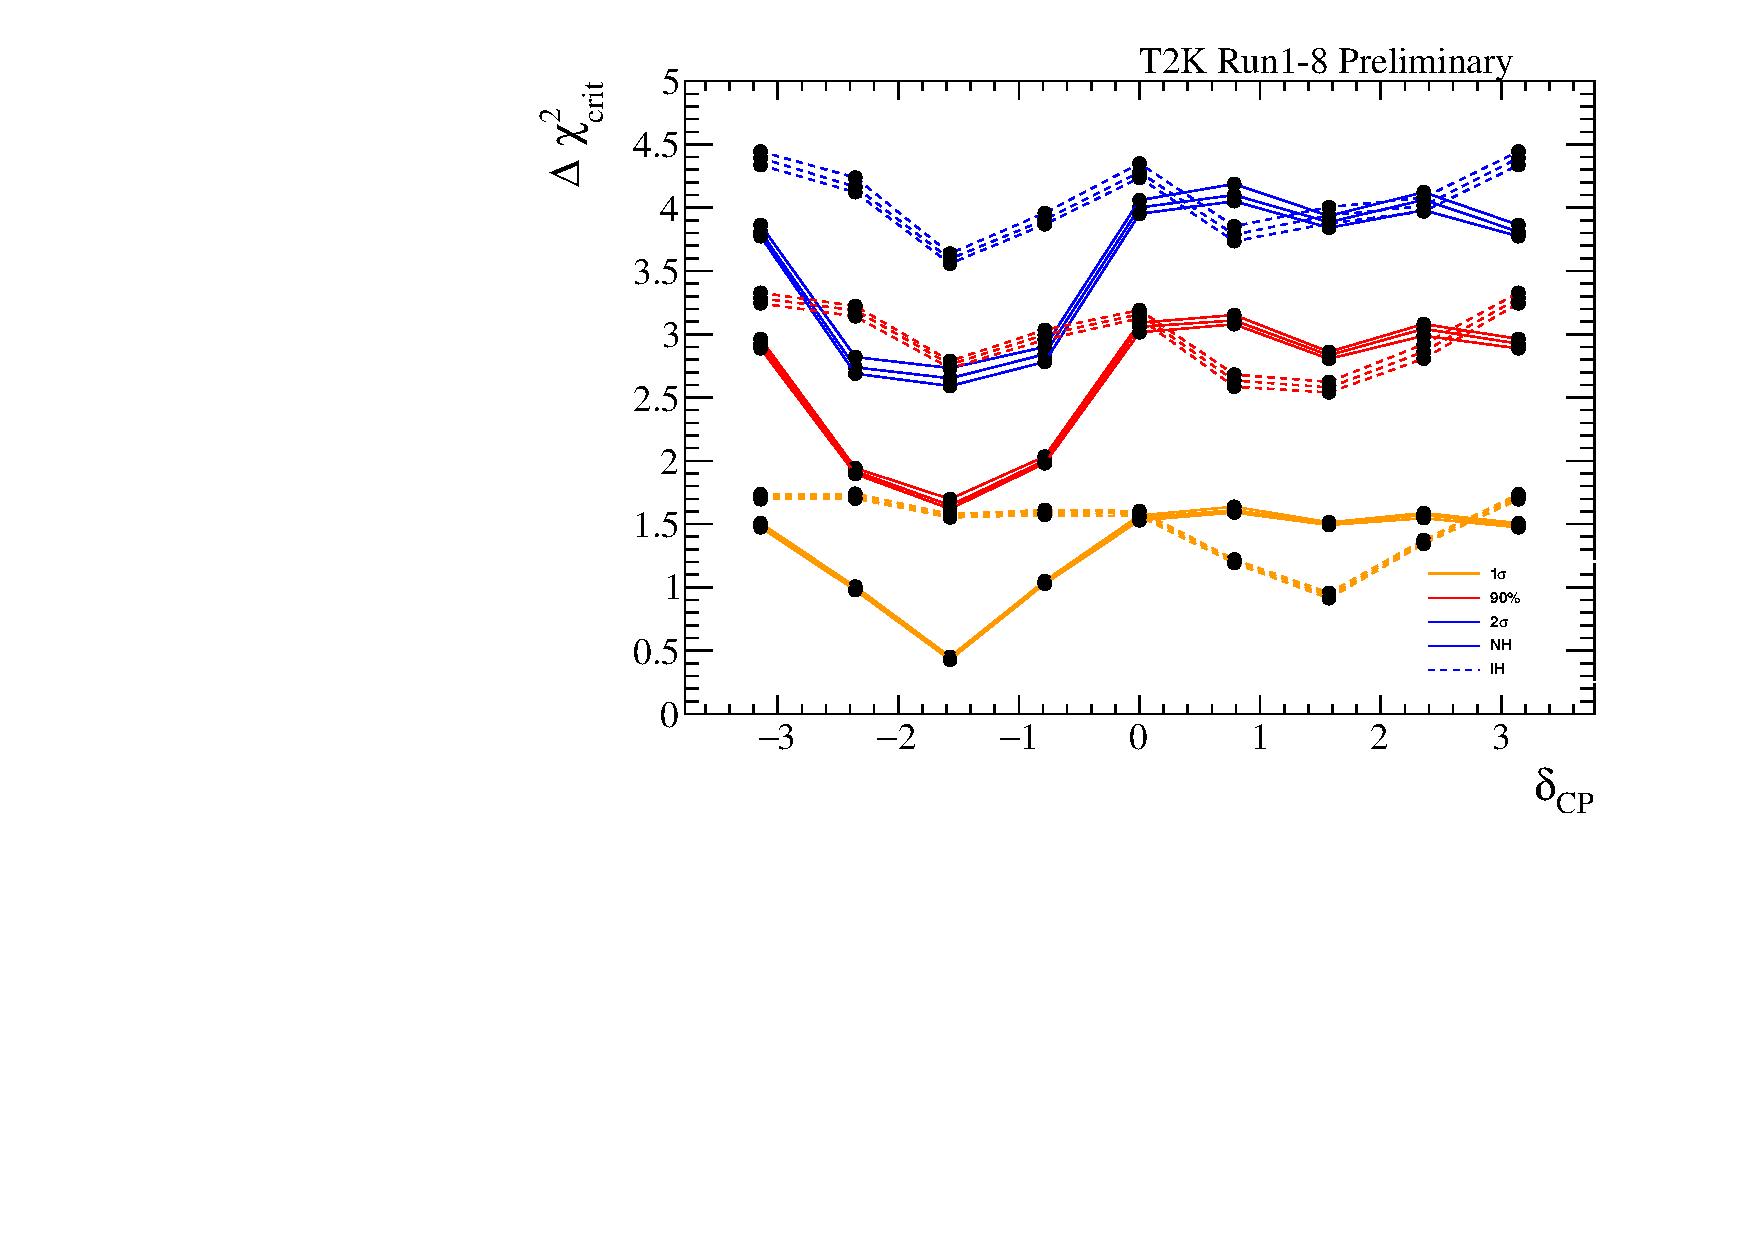
\includegraphics[width=0.9\textwidth]{data/fc/2017b/FC_critical_values}
		\caption{\label{fig:fc_critval_2017b}Critical $\Delta\chi^2$ values}
	\end{subfigure}
	\begin{subfigure}[b]{0.49\textwidth}
		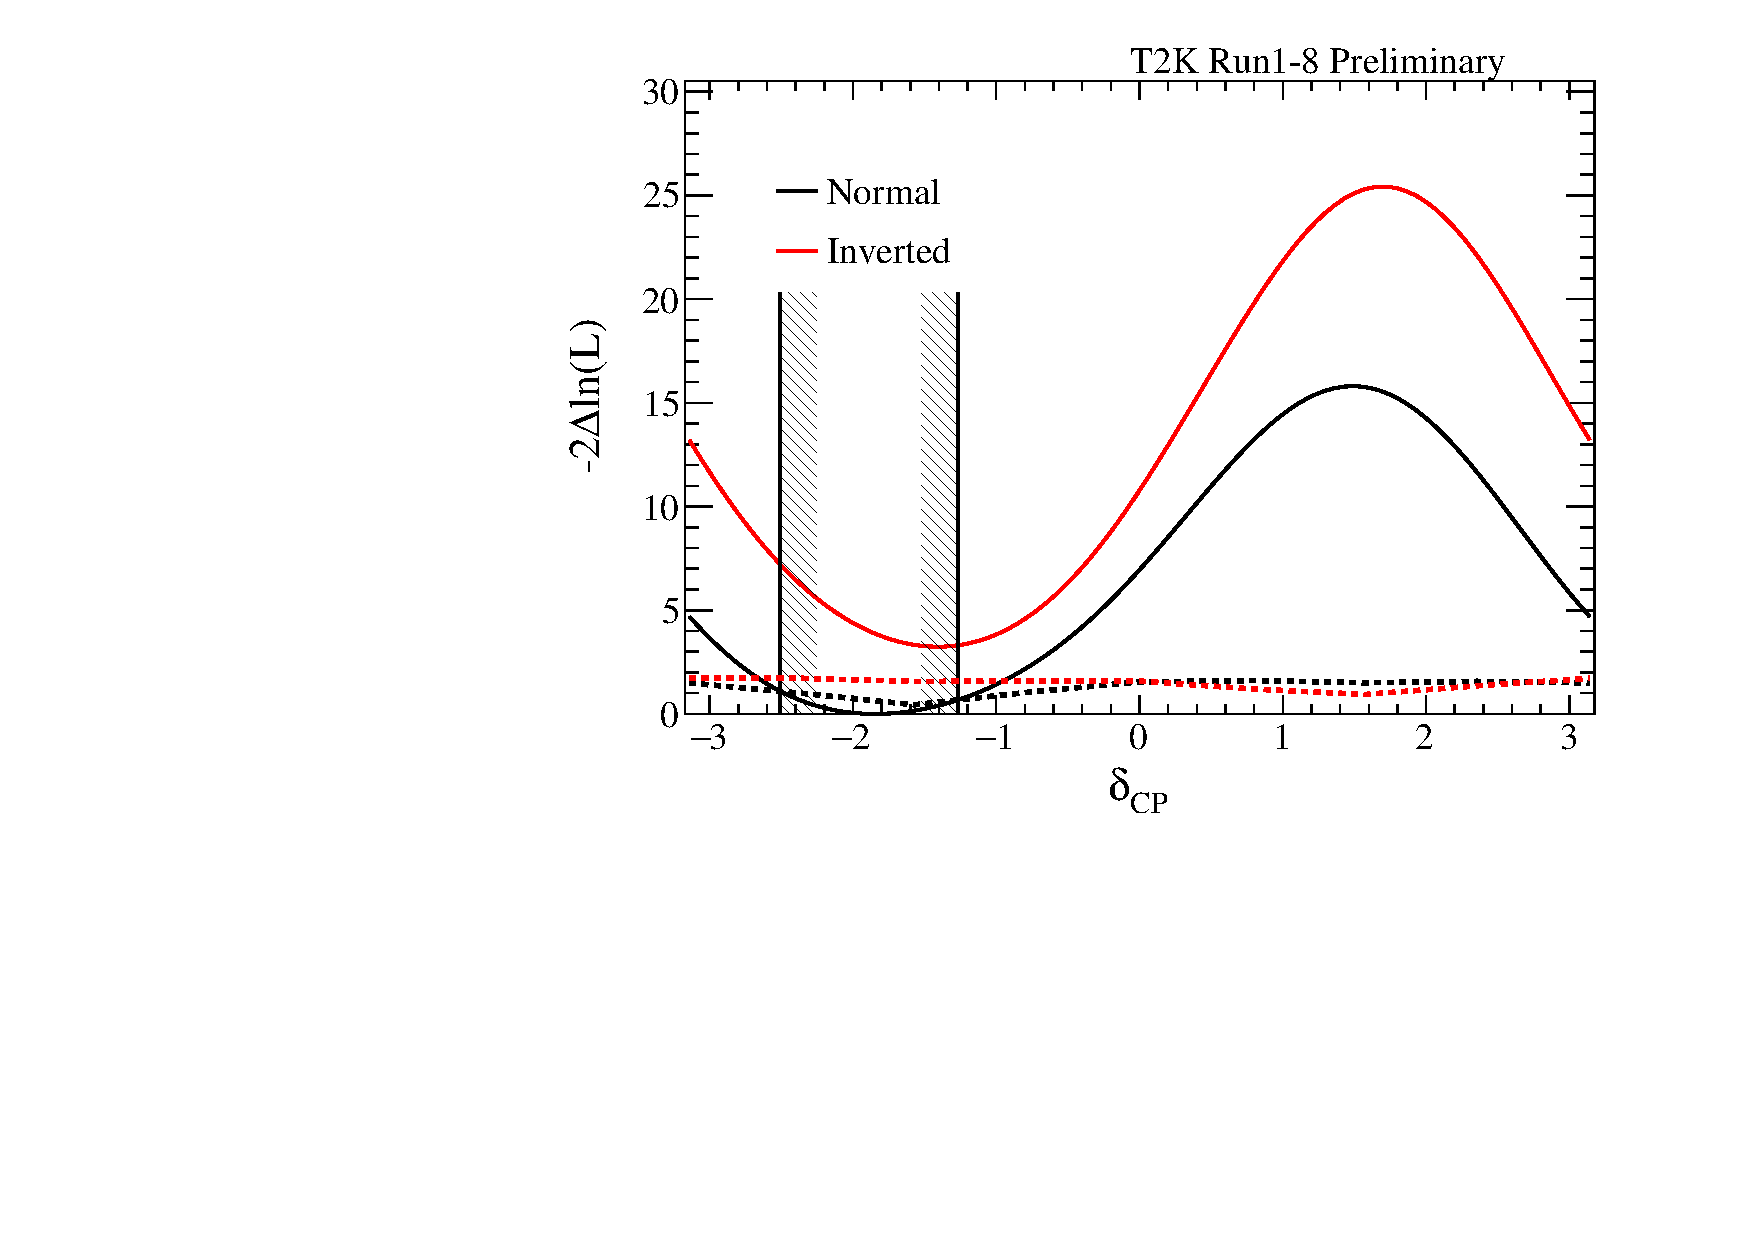
\includegraphics[width=0.9\textwidth]{data/fc/2017b/deltacp_FC_1sigma_CL}
		\caption{$1\sigma$ CL exclusion region}
	\end{subfigure}
	\begin{subfigure}[b]{0.49\textwidth}
		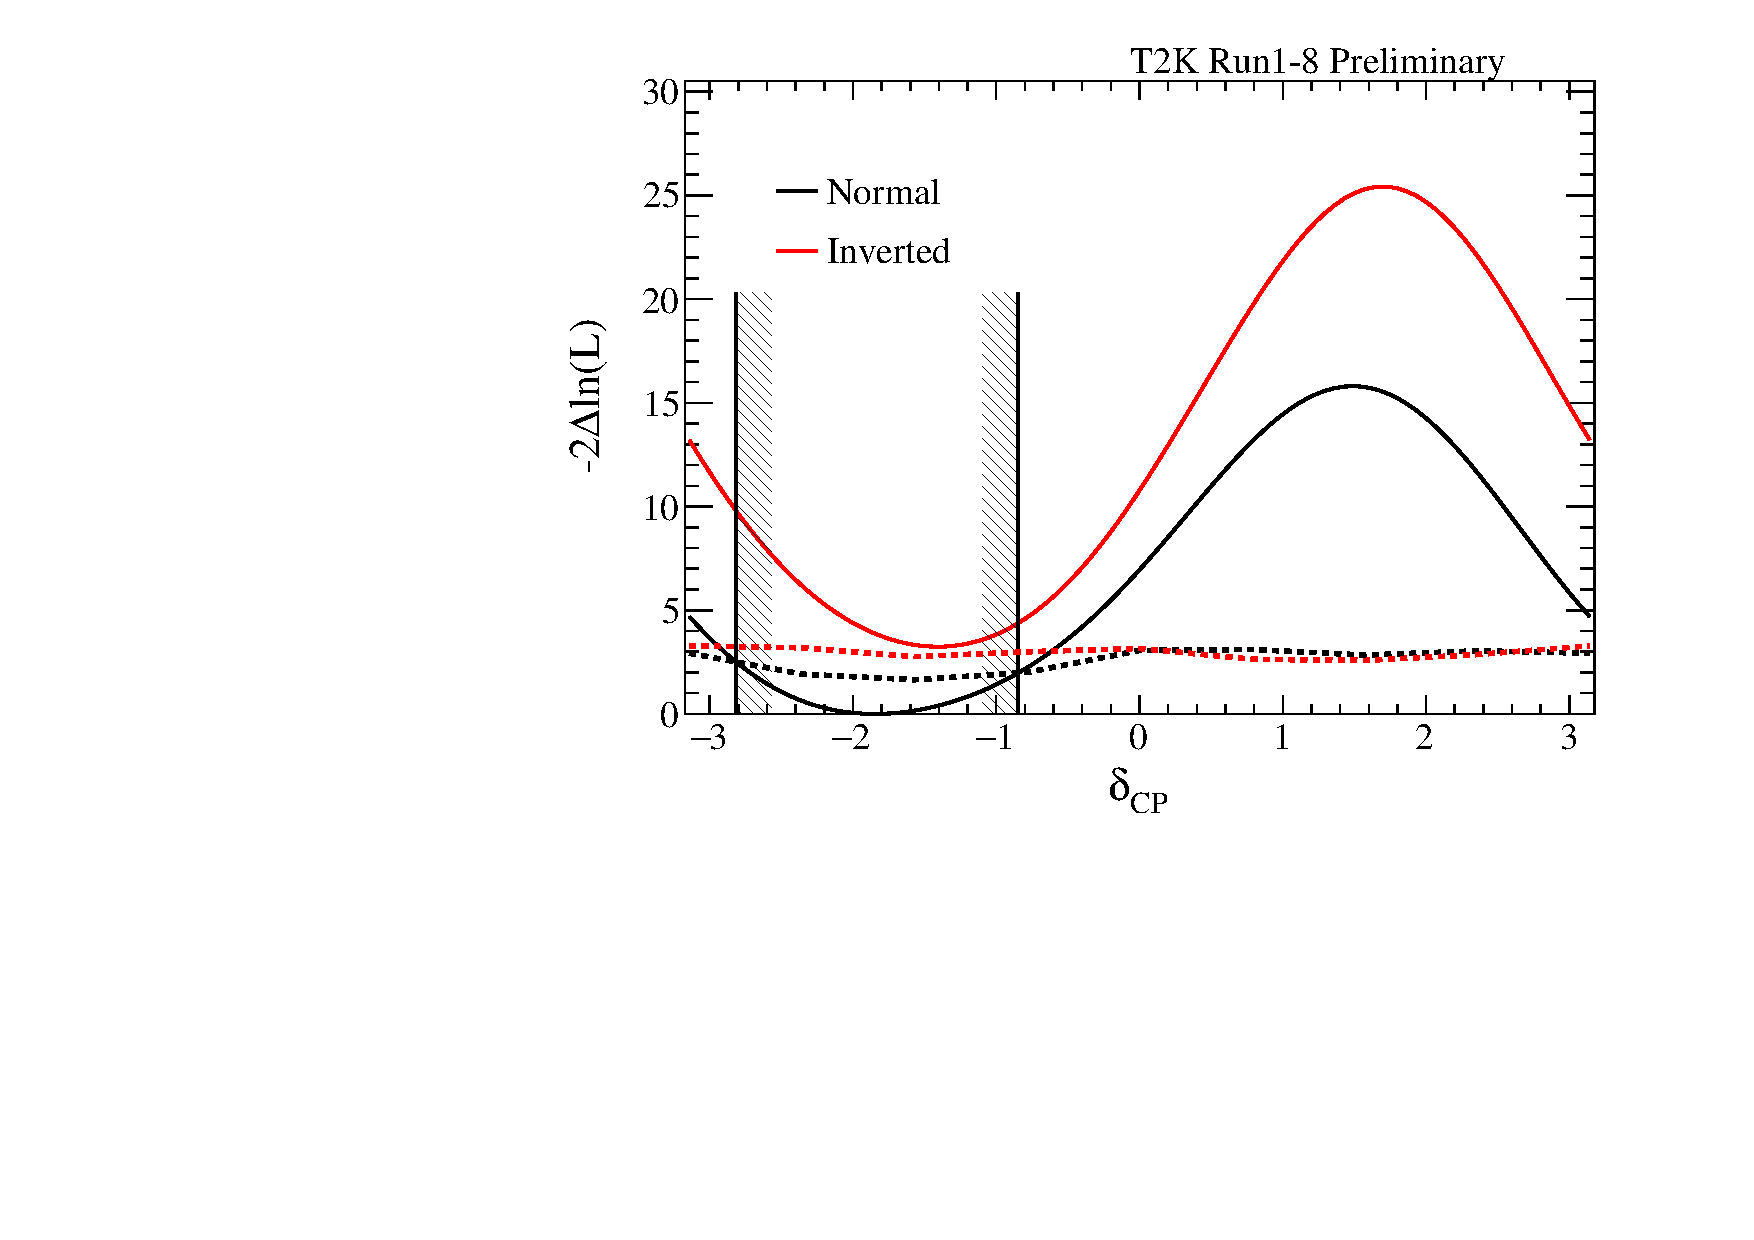
\includegraphics[width=0.9\textwidth]{data/fc/2017b/deltacp_FC_90_CL}
		\caption{90\% CL exclusion region}
	\end{subfigure}
	\begin{subfigure}[b]{0.49\textwidth}
		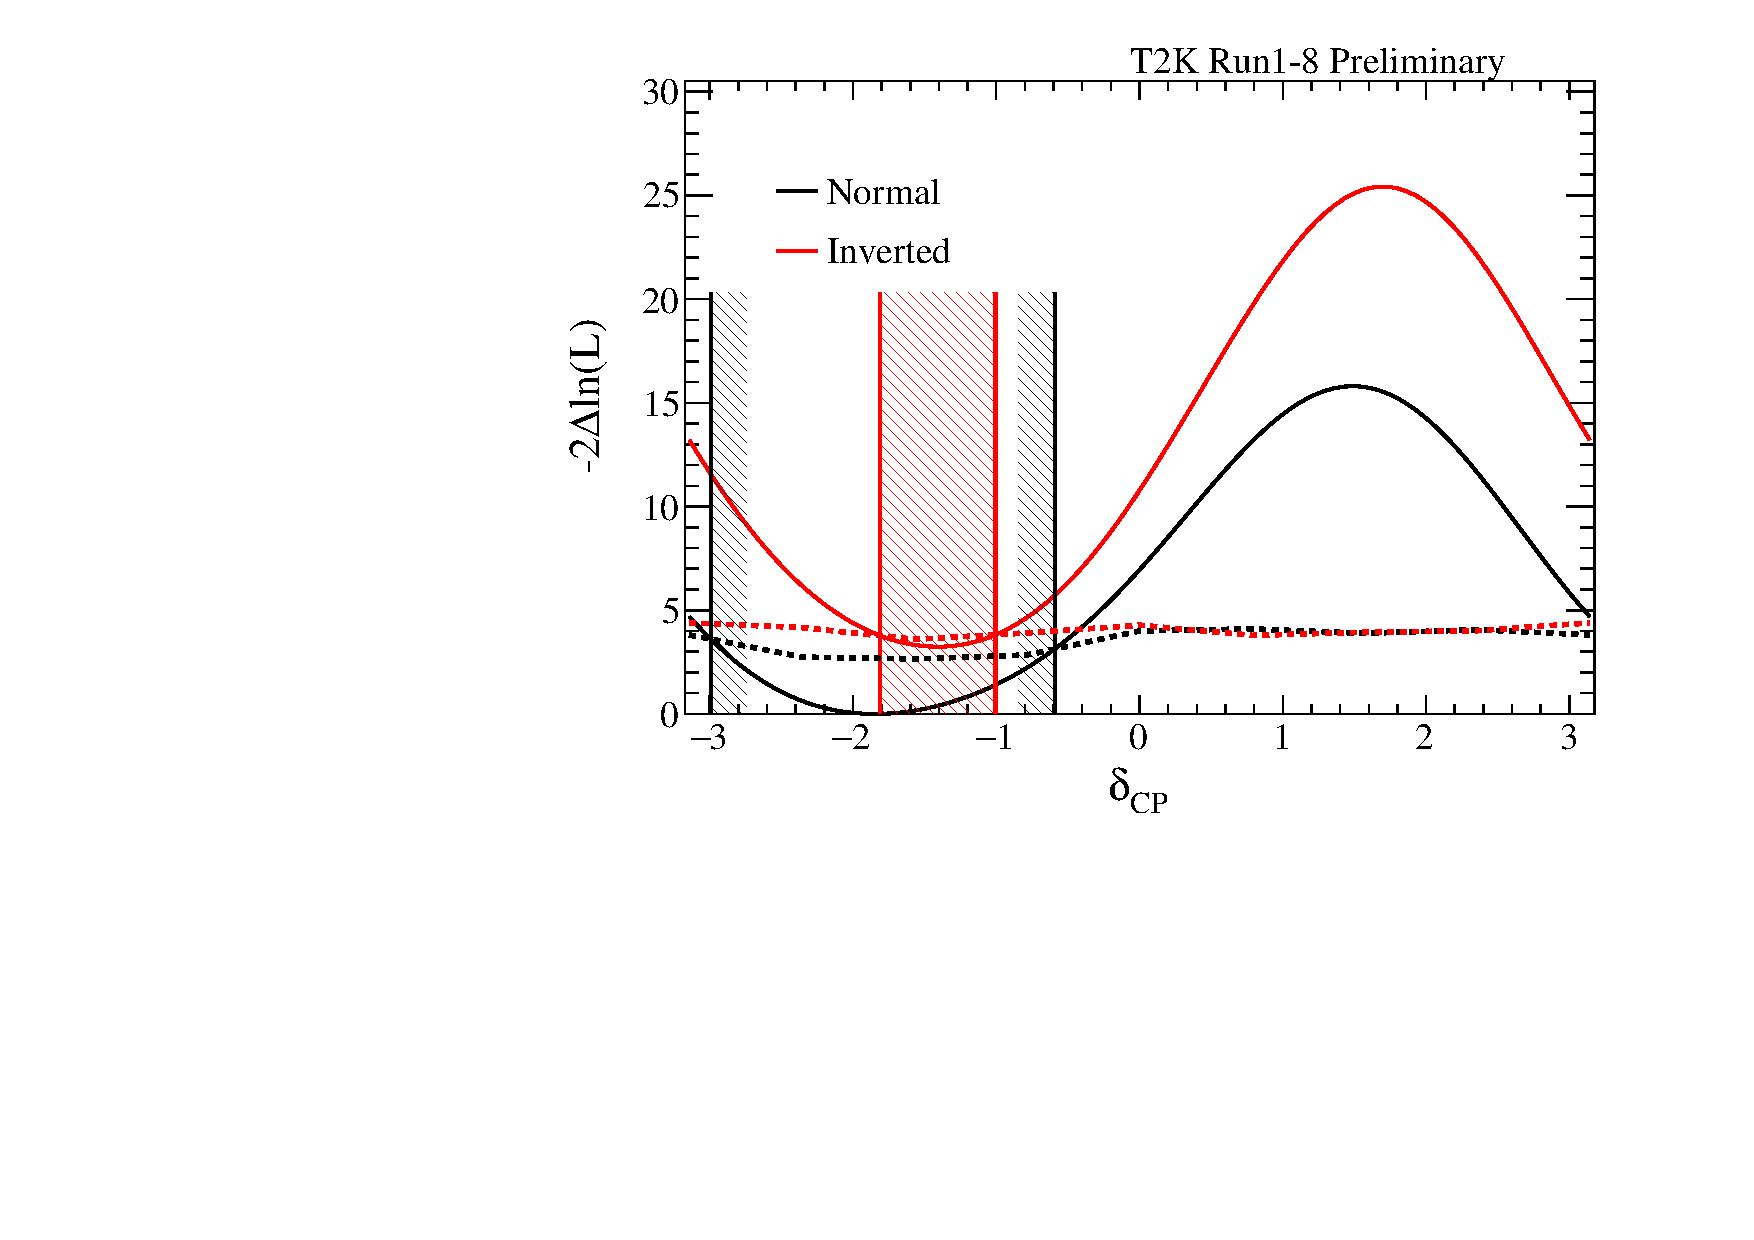
\includegraphics[width=0.9\textwidth]{data/fc/2017b/deltacp_FC_2sigma_CL}
		\caption{$2\sigma$ CL exclusion region}
	\end{subfigure}
	\caption {
$\Delta\chi^2$ critical values and confidence intervals for the measured $\Delta\chi^2$ distributions for \RunPeriod. Critical values obtained with the Feldman-Cousins method for \RunPeriod for 9 evenly spaced values on the range \( \left[-\pi,\pi\right] \). Critical values are shown for 1\( \sigma \), 2\( \sigma \) and 90\% CL for normal (solid lines) and inverted (dashed lines) hierarchies. At least \num{1e4} toy experiments are performed for each point. The three bands of lines show the \( \pm 1\sigma \) uncertainty on the critical values. Also shown are the measured \( \Delta \chi^2 \) distributions shifted with respect to the same global minium and the $1\sigma$, 90\% and $2\sigma$ exclusion regions for both mass hierarchies. 
	}
	\label{fig:fc_interval_2017b}
\end{figure*}

\begin{table}[htb]
	\centering
	\begin{tabular}{| c | c | c | c | c |}
\hline
Parameter & Reactor & CL & Normal hierarchy & Inverted hierarchy \\
\hline
\deltacp		& Yes & 90\% & $\left[ -2.815, -0.847 \right]$ & - \\
\deltacp		& Yes & $ 2\sigma $ & $\left[ -2.992, -0.592 \right]$ & $\left[ -1.808, -1.005 \right]$ \\
\hline
\end{tabular}

	\caption{
		The confidence intervals at 90\% CL and $2\sigma$ CL obtained with the Feldman-Cousins method for the \RunPeriod data set is shown for the measurement of \deltacp versus mass hierarchy.
	}
	\label{tab:fc_interval_2017b}
\end{table}

\subsubsection{$\delta_{CP} = -\pi/2$ - normal hierarchy}

In \cref{fig:brazilian_dcp_mpi2_2017b} the \RunPeriod data result for \deltacp versus mass hierarchy is compared to \color{blue}68.27\% and 95.45\% of toys from a $\Delta\chi^2$ distribution\color{black} corresponding to $\delta_{CP} = -\pi/2$ and (a) normal hierarchy and (b) inverted hierarchy. \color{blue}We see that more than 4.45\% ($2\sigma$ level) of toys provide a stronger constraint than the data contour for both normal and inverted hierarchy, consistent with the PMNS matrix\color{black}.

\color{blue}We also see an interesting feature near $\delta_{CP} = -\pi/2$ where the $\Delta\chi^2$ values have a wider distribution. This is due to the boundary at $\delta_{CP} = -\pi/2$ which causes a wider distribution when the parameter \deltacp would like to be pushed beyond the boundary in the fit.\color{black}

Finally from \cref{fig:brazilian_dcp_mpi2_2017b}(c) we see that $\delta_{CP} = 0$ and $\delta_{CP} = \pi$ are excluded at 90\% confidence level at between 40\% and 50\% (see \cref{tab:exclusion_prob_2017b}) of the toy experiments and excluded at $2\sigma$ confidence level in between 25\% and 35\% of the toy experiments, with $\delta_{CP} = \pi$ excluded in slightly fewer toy experiments in each case.

\begin{figure*}[htb]
	\center
	\begin{subfigure}[b]{0.49\textwidth}
		\includegraphics[width=0.9\textwidth]{comparison/2017b/dcp_run18_react_Data_braz_nh}
		\caption{Normal hierarchy}
	\end{subfigure}
	\begin{subfigure}[b]{0.49\textwidth}
		\includegraphics[width=0.9\textwidth]{comparison/2017b/dcp_run18_react_Data_braz_ih}
		\caption{Inverted hierarchy}
	\end{subfigure}
	\begin{subfigure}[b]{0.49\textwidth}
		\includegraphics[width=0.9\textwidth]{comparison/2017b/dcp_run18_react_Data_prob_chisq}
		\caption{Data \(\Delta \chi^2\) probability }
	\end{subfigure}
	\caption {
		The distribution of $\Delta\chi^2$ vs \deltacp obtained with \num{1e4} toy experiments generated with $\delta_{CP} = -\pi/2$ and normal hierarchy is shown. The $\Delta\chi^2$ distributions obtained by fixing the mass hierarchy to normal (left) and inverted (right) are shown, along with the $\Delta\chi^2$ values corresponding to 68.27\% and 95.45\% of the toy experiments and the average $\Delta\chi^2$ values from all experiments. Also shown are the fractions of toys which exclude each value of \deltacp to 90\% and $2\sigma$ using the Feldman-Cousins corrected critical values (bottom).
	}
	\label{fig:brazilian_dcp_mpi2_2017b}
\end{figure*}

\begin{table}[htb]
	\centering
	\begin{tabular}{| c | c | c | c |}
\hline
\deltacp & Hierarchy & 90\% & $2\sigma$ \\
\hline
0		& NH & 0.474 & 0.332 \\
$\pi$	& NH & 0.414 & 0.279 \\
0		& IH & 0.803 & 0.708 \\
$\pi$	& IH & 0.796 & 0.693 \\
\hline
\end{tabular}

	\caption{
		The fraction of toy experiments for which $\delta_{CP} = 0, \pi$ and normal and inverted hierarchy are excluded at 90\% and $2\sigma$ CL is shown. 10k toy experiments are used.
	}
	\label{tab:exclusion_prob_2017b}
\end{table}

\clearpage

\subsection{Comparison to 2017 results}
\label{sec:results:comparison}

This section presents comparisons of the updated fits with the 2017 fits described in \cref{sec:results} for the case of reactor fits (except in the case of \ssqthonethree, which does not apply the reactor constraint).

\subsubsection{Results for \appearance}
In \cref{fig:ssqth13_vs_dcp_data_compare} the result for \appearance with reactor constraint.

\begin{figure*}[htb]
	\center
	\begin{subfigure}[b]{0.49\textwidth}
		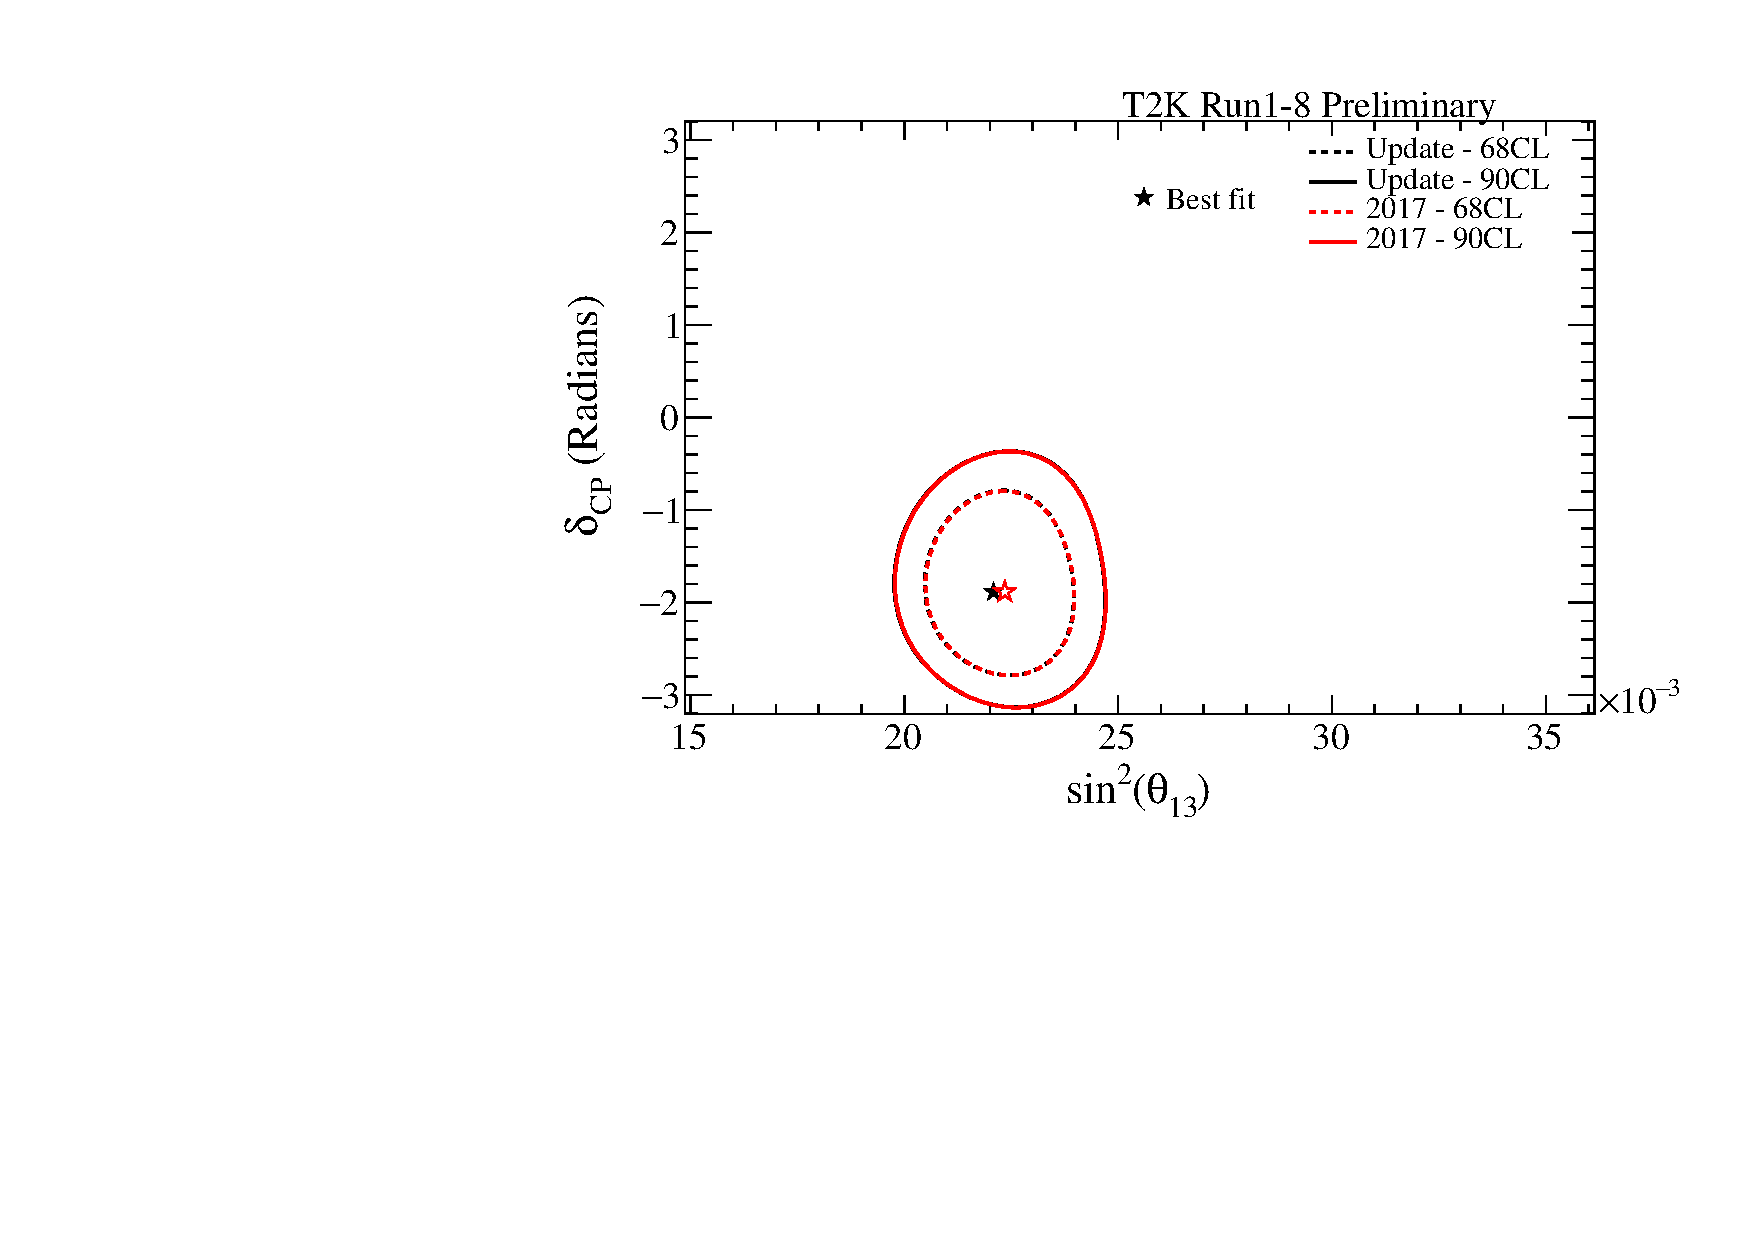
\includegraphics[width=0.9\textwidth]{data/reactor/2017b/comparisons/mixing13_deltacp_data_reactor_nh}
		\caption{\appearance NH}
	\end{subfigure}
	\begin{subfigure}[b]{0.49\textwidth}
		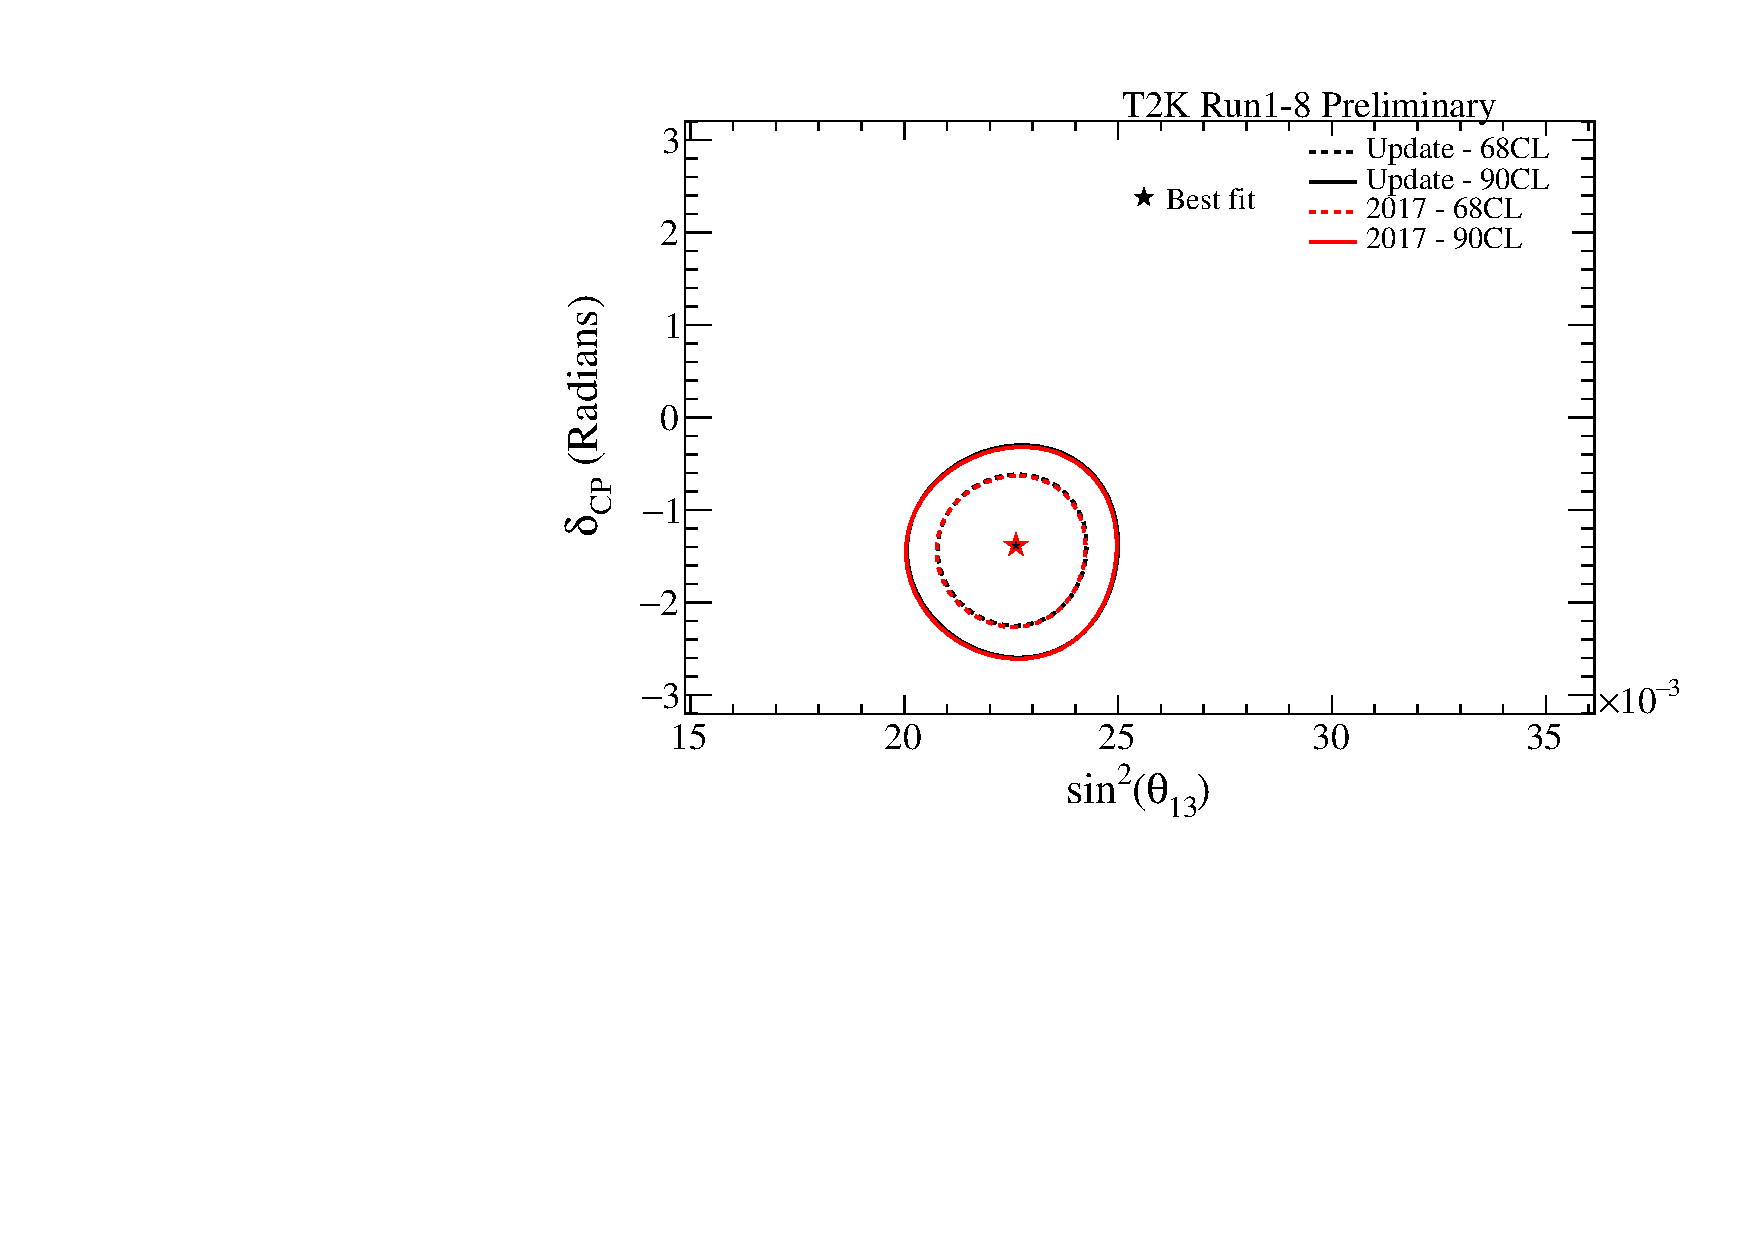
\includegraphics[width=0.9\textwidth]{data/reactor/2017b/comparisons/mixing13_deltacp_data_reactor_ih}
		\caption{\appearance IH}
	\end{subfigure}
	\caption {
		Contours at 68\% and 90\% CL for \appearance with reactor constraint. Normal and inverted hierarchy contours are independent. All 5 samples were used to produce these fits.
	}
	\label{fig:ssqth13_vs_dcp_data_compare}
\end{figure*}

\subsubsection{Results for \disappearance}

The result for \disappearance with reactor constraint is shown in fig.~\ref{fig:ssqth23_vs_dmsq23_data_compare}.

\begin{figure*}[htb]
	\center
	\begin{subfigure}[b]{0.49\textwidth}
		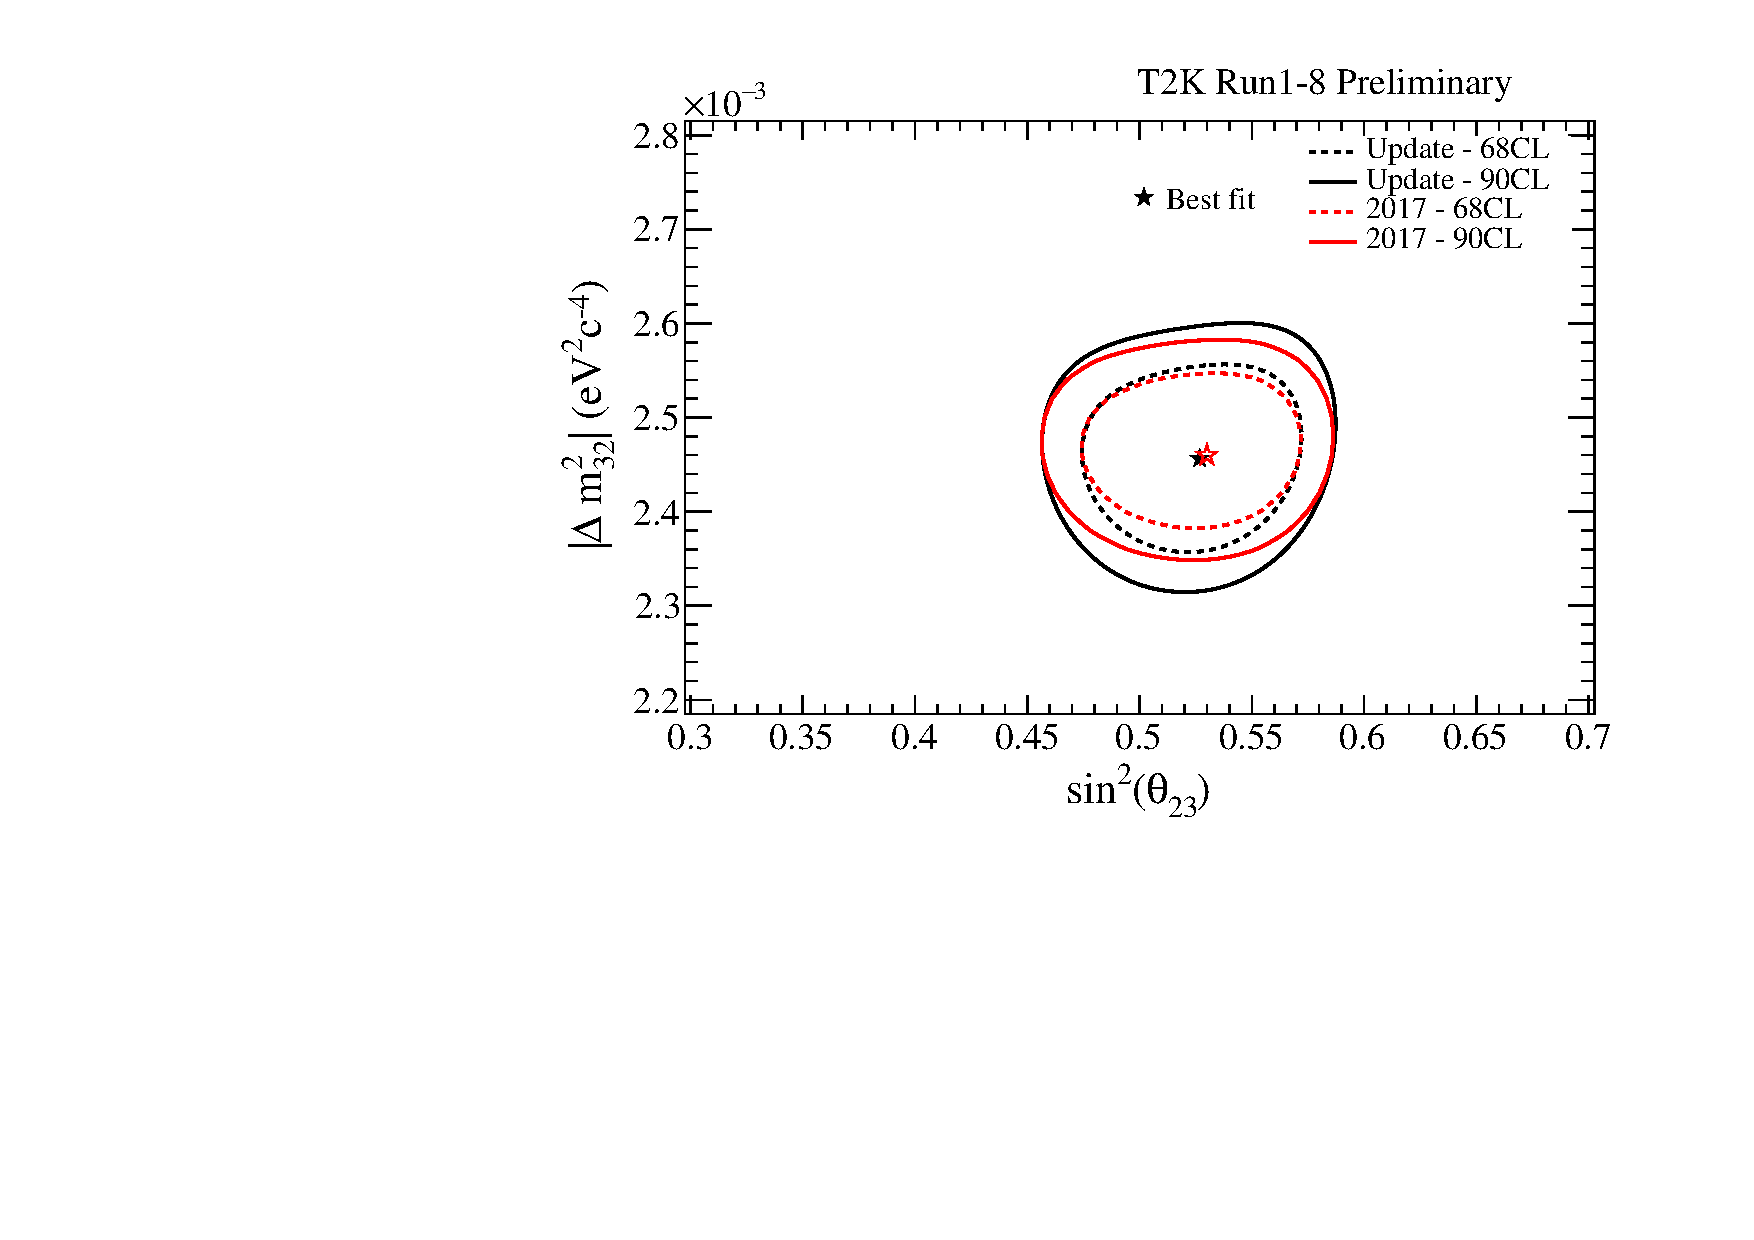
\includegraphics[width=0.9\textwidth]{data/reactor/2017b/comparisons/mixing23_dmsq23_data_reactor_nh}
		\caption{\disappearance NH}
	\end{subfigure}
	\begin{subfigure}[b]{0.49\textwidth}
		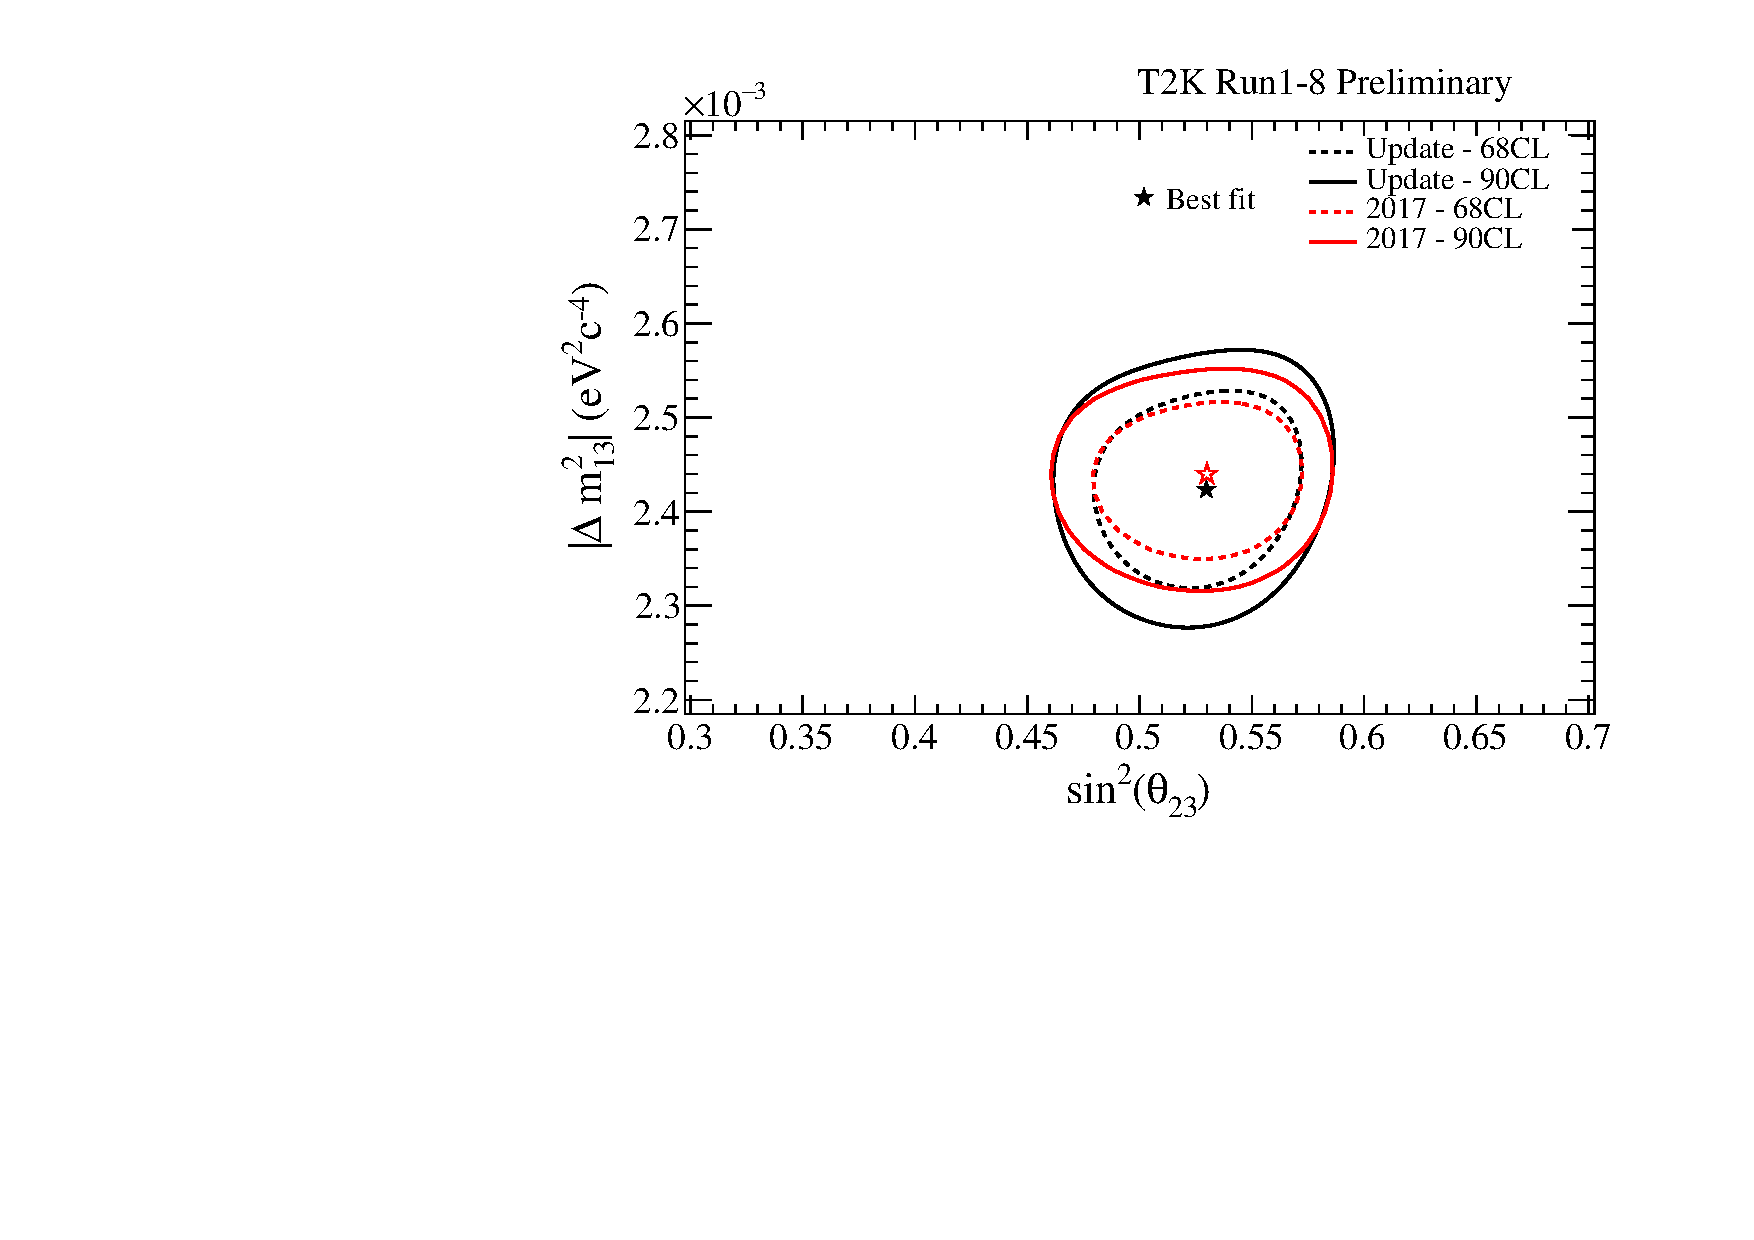
\includegraphics[width=0.9\textwidth]{data/reactor/2017b/comparisons/mixing23_dmsq23_data_reactor_ih}
		\caption{\disappearance IH}
	\end{subfigure}
	\caption {
		Contours at 68\% and 90\% CL for \disappearance with reactor constraint. Normal and inverted hierarchy contours are independent. All 5 samples were used to produce these fits.
	}
	\label{fig:ssqth23_vs_dmsq23_data_compare}
\end{figure*}

\clearpage

\subsubsection{Results for \deltacp}

The result for \deltacp with reactor constraint is shown in fig.~\ref{fig:dcp_data_compare}.

\begin{figure*}[htb]
	\center
	\begin{subfigure}[b]{0.49\textwidth}
		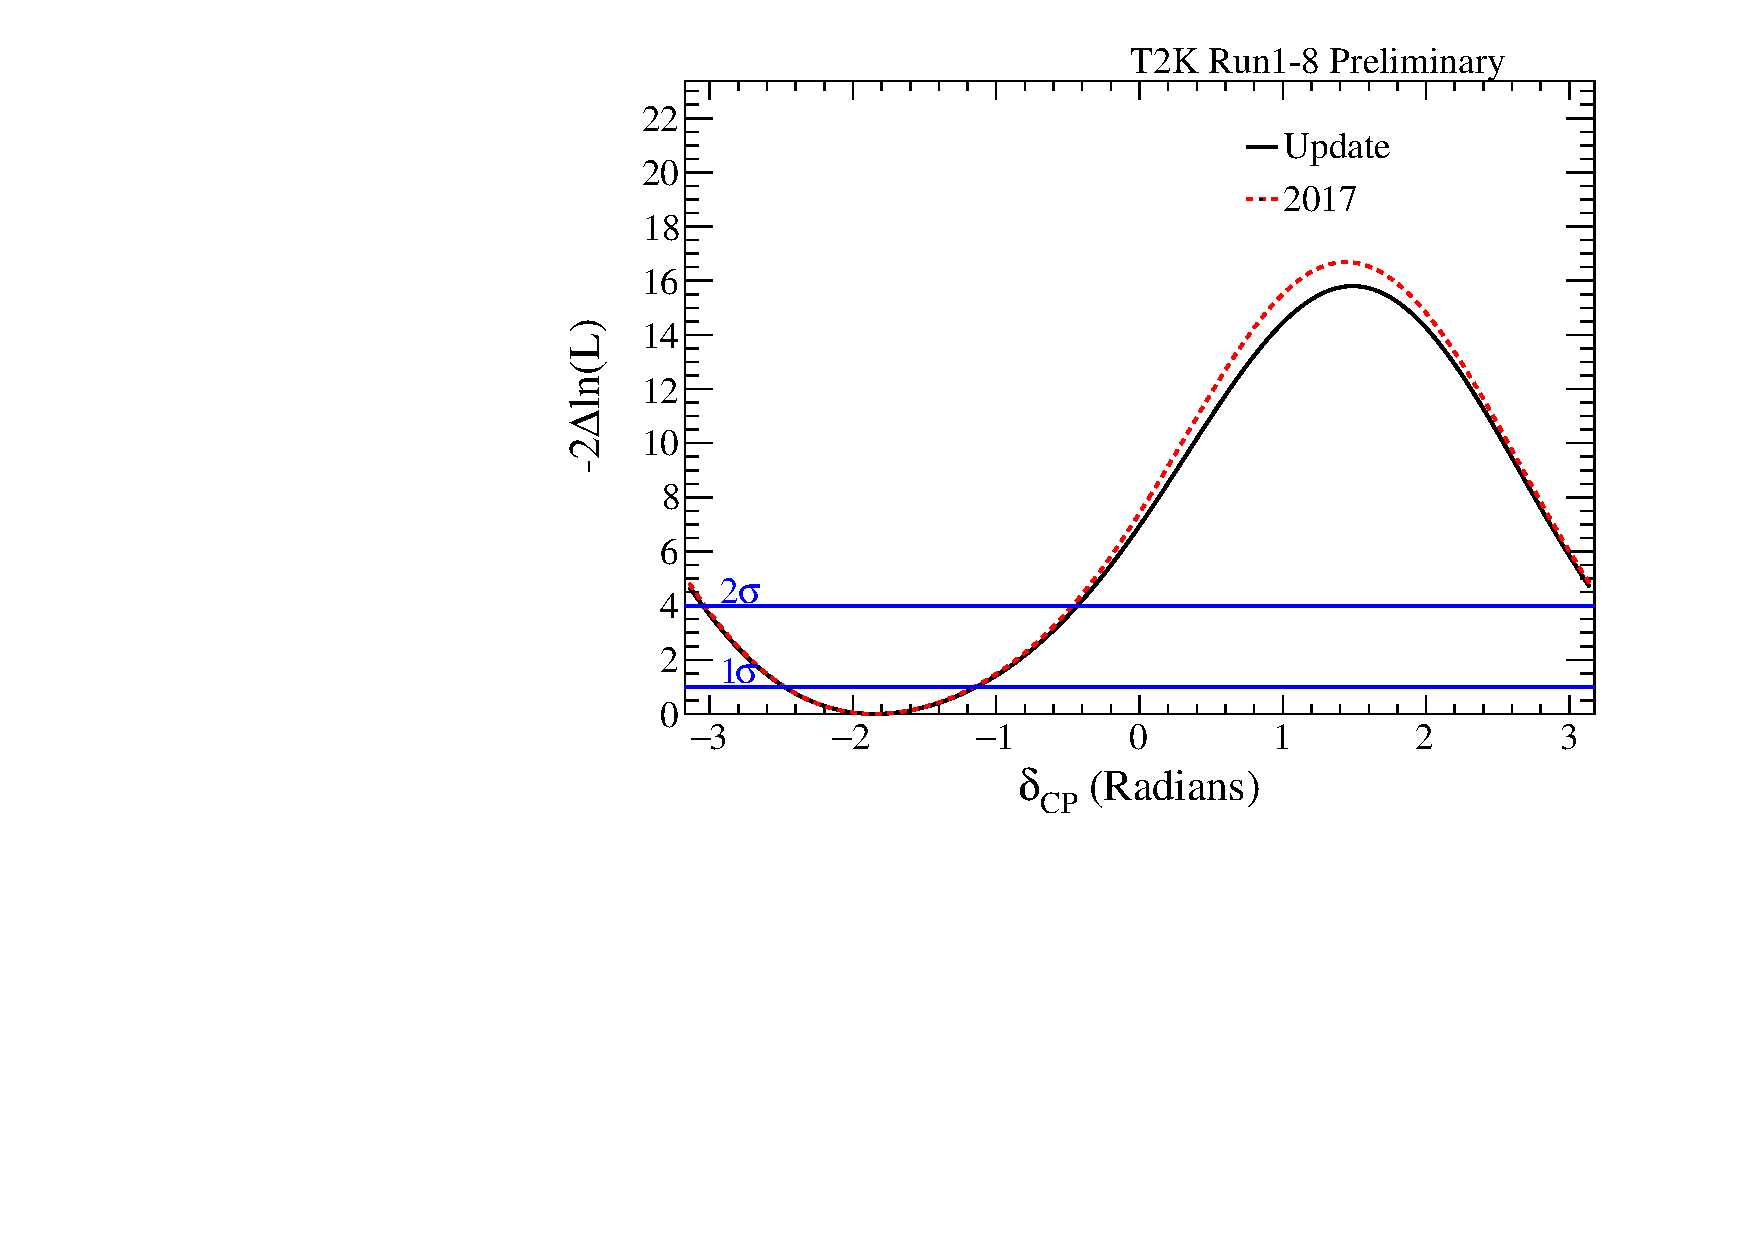
\includegraphics[width=0.9\textwidth]{data/reactor/2017b/comparisons/deltacp_data_reactor_nh}
		\caption{\deltacp NH}
	\end{subfigure}
	\begin{subfigure}[b]{0.49\textwidth}
		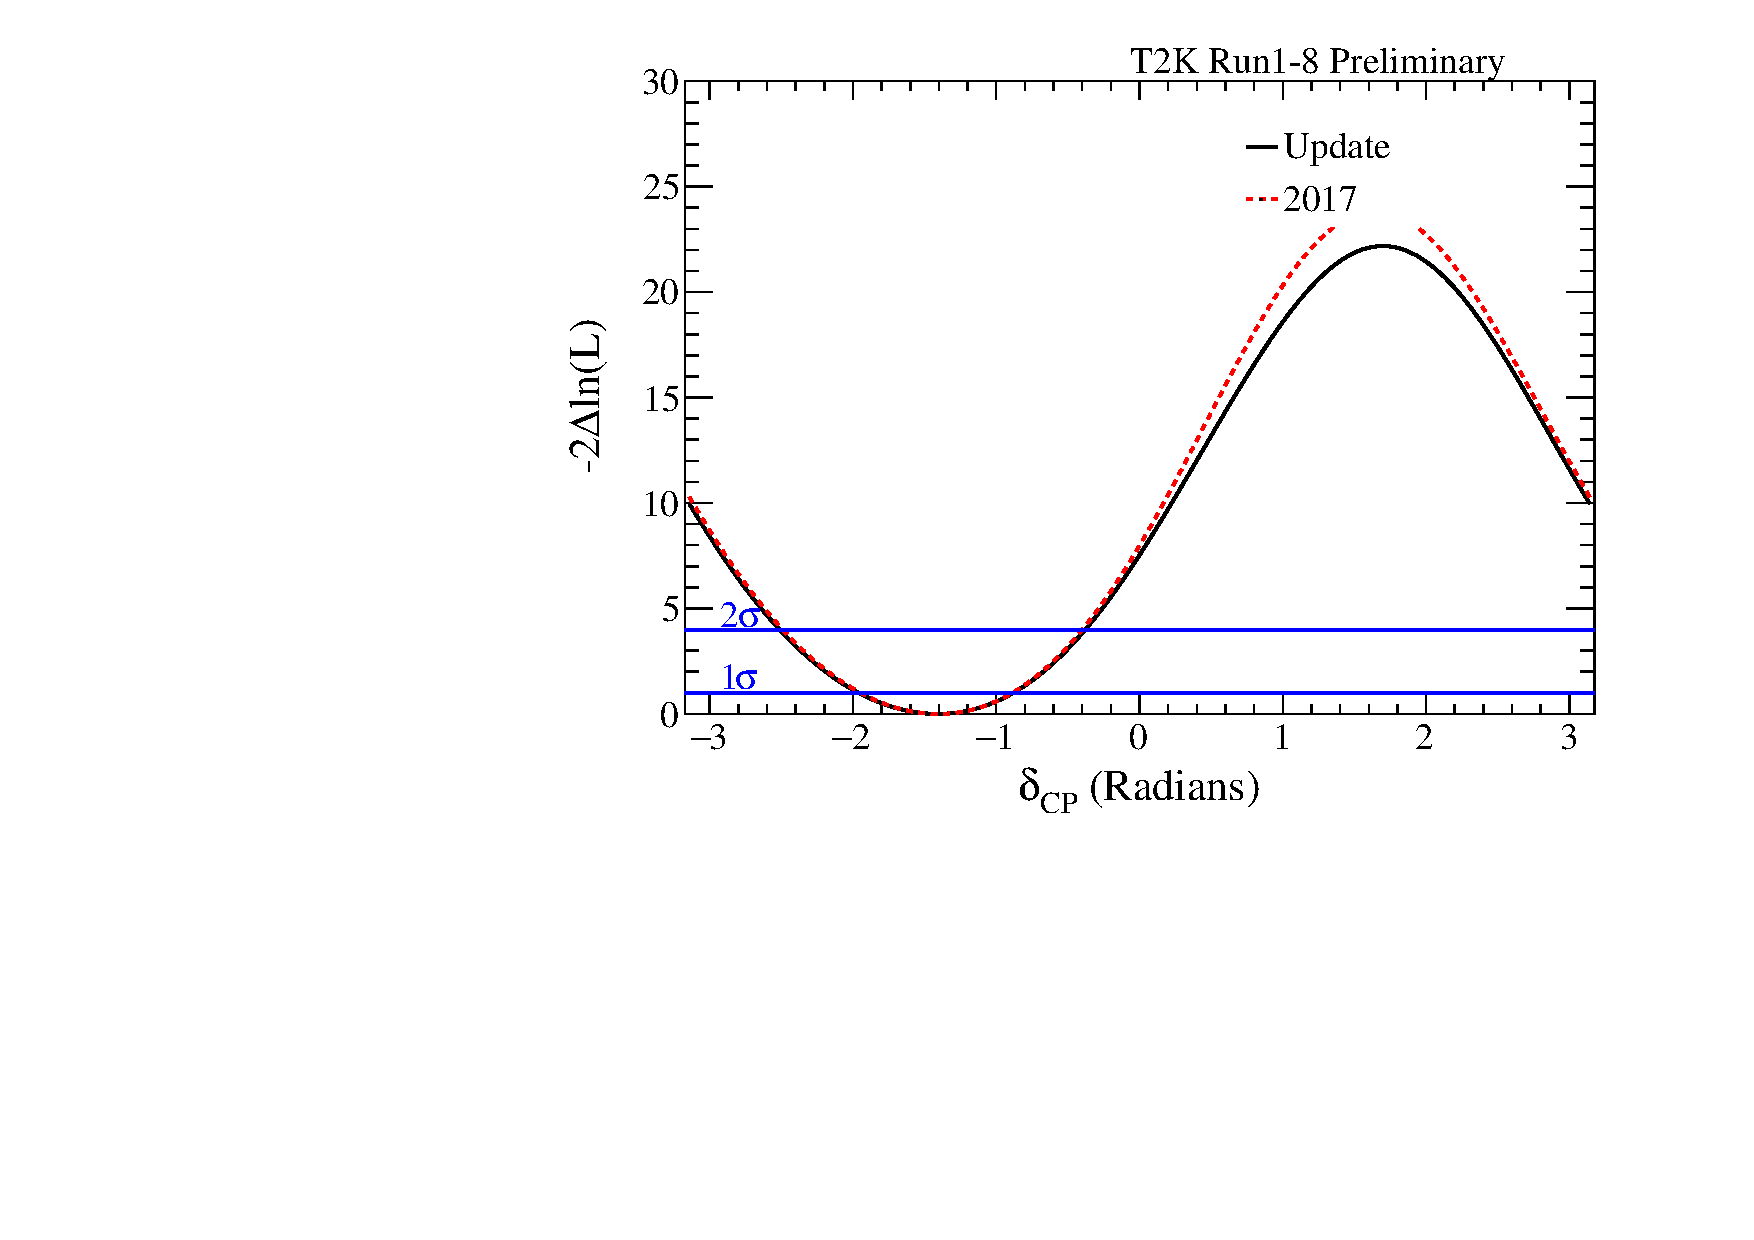
\includegraphics[width=0.9\textwidth]{data/reactor/2017b/comparisons/deltacp_data_reactor_ih}
		\caption{\deltacp IH}
	\end{subfigure}
	\caption {
		The expected $\Delta\chi^2$ distribution as a function of \deltacp with reactor constraint. The mass hierarchy is minimized, with normal and inverted hierarchy $\Delta\chi^2$ distributions shifted to the same global best-fit $\chi^2$ value, which is taken to be the minimum between normal and inverted hierarchy. All 5 samples were used to produce these fits.
	}
	\label{fig:dcp_data_compare}
\end{figure*}

\subsubsection{Results for \ssqthonethree}

The result for \ssqthonethree (without reactor constraint) is shown in fig.~\ref{fig:th13_data_compare}.

\begin{figure*}[htb]
	\center
	\begin{subfigure}[b]{0.49\textwidth}
		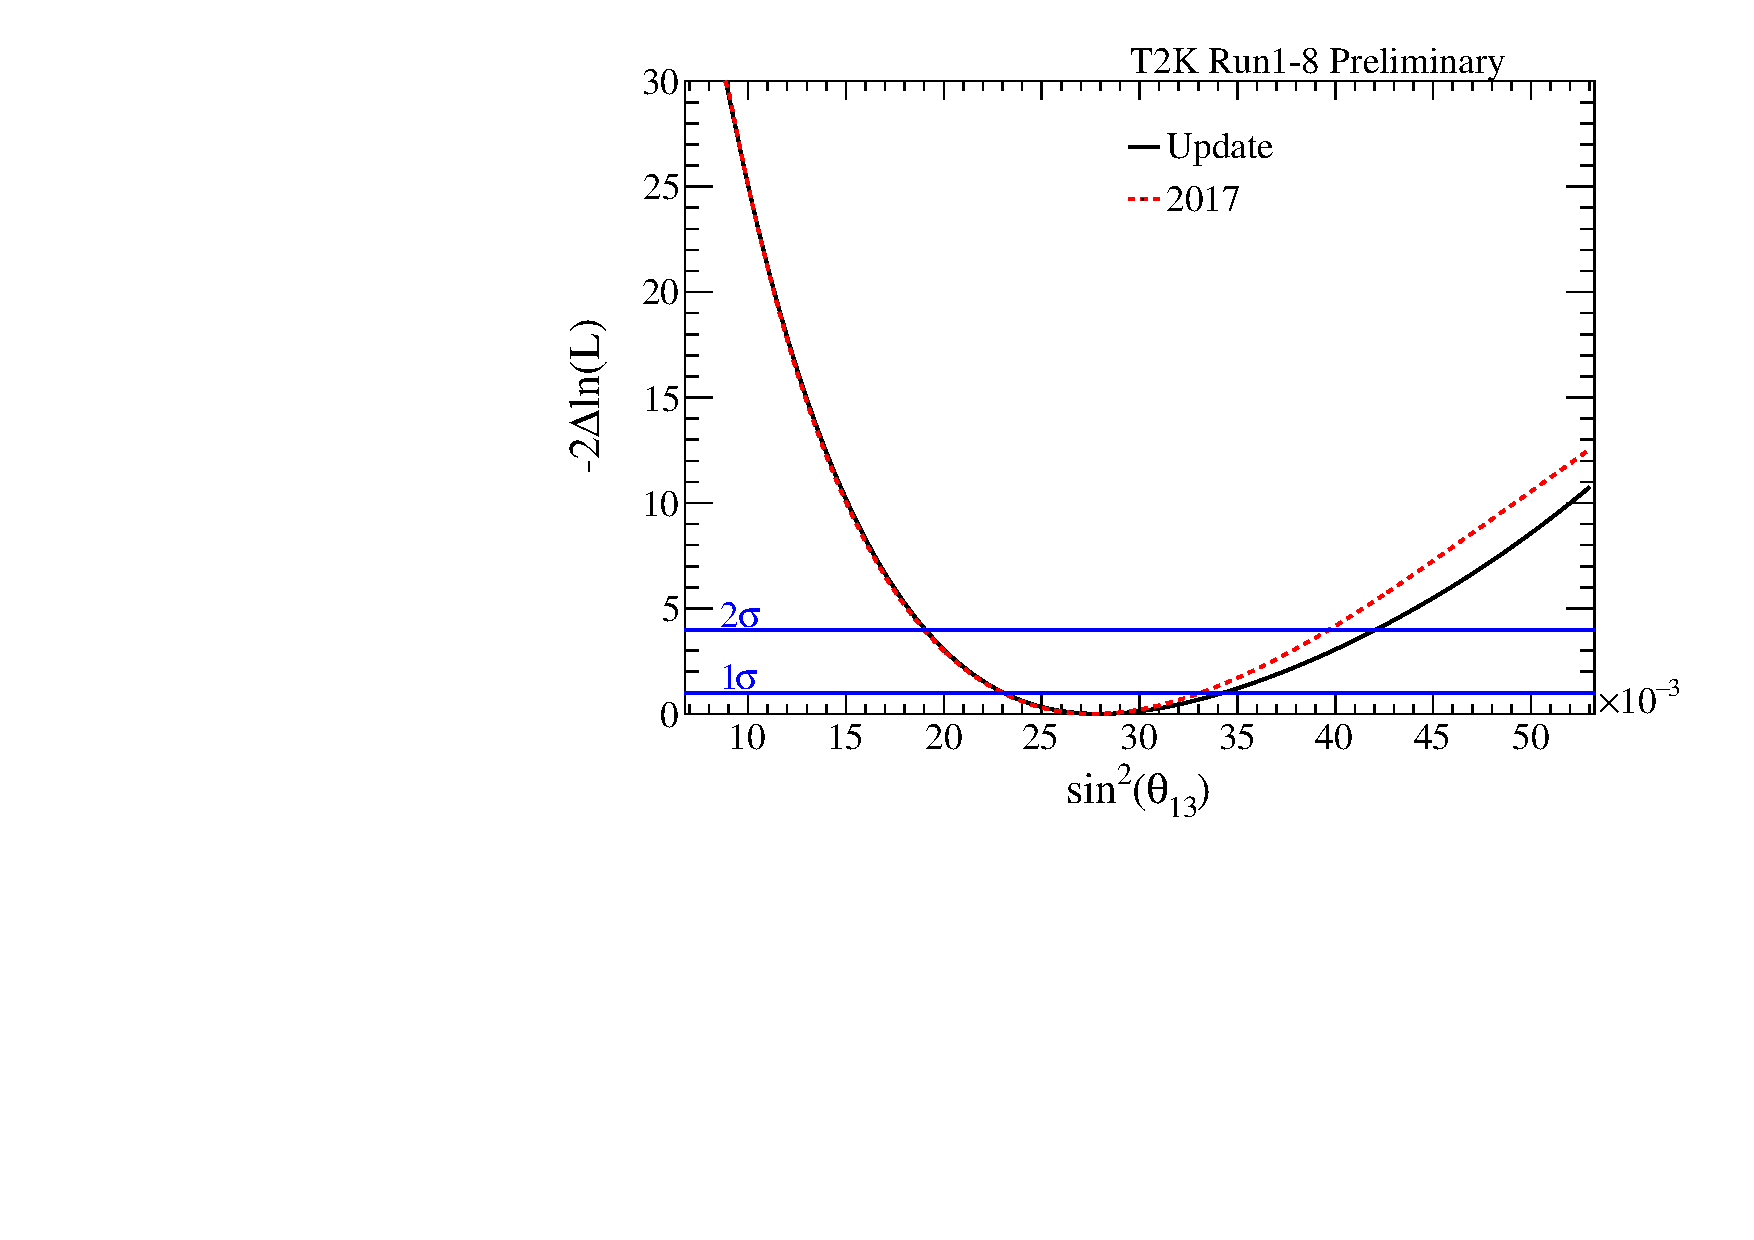
\includegraphics[width=0.9\textwidth]{data/t2k/2017b/comparisons/mixing13_data_t2k_nh}
		\caption{\ssqthonethree NH}
	\end{subfigure}
	\begin{subfigure}[b]{0.49\textwidth}
		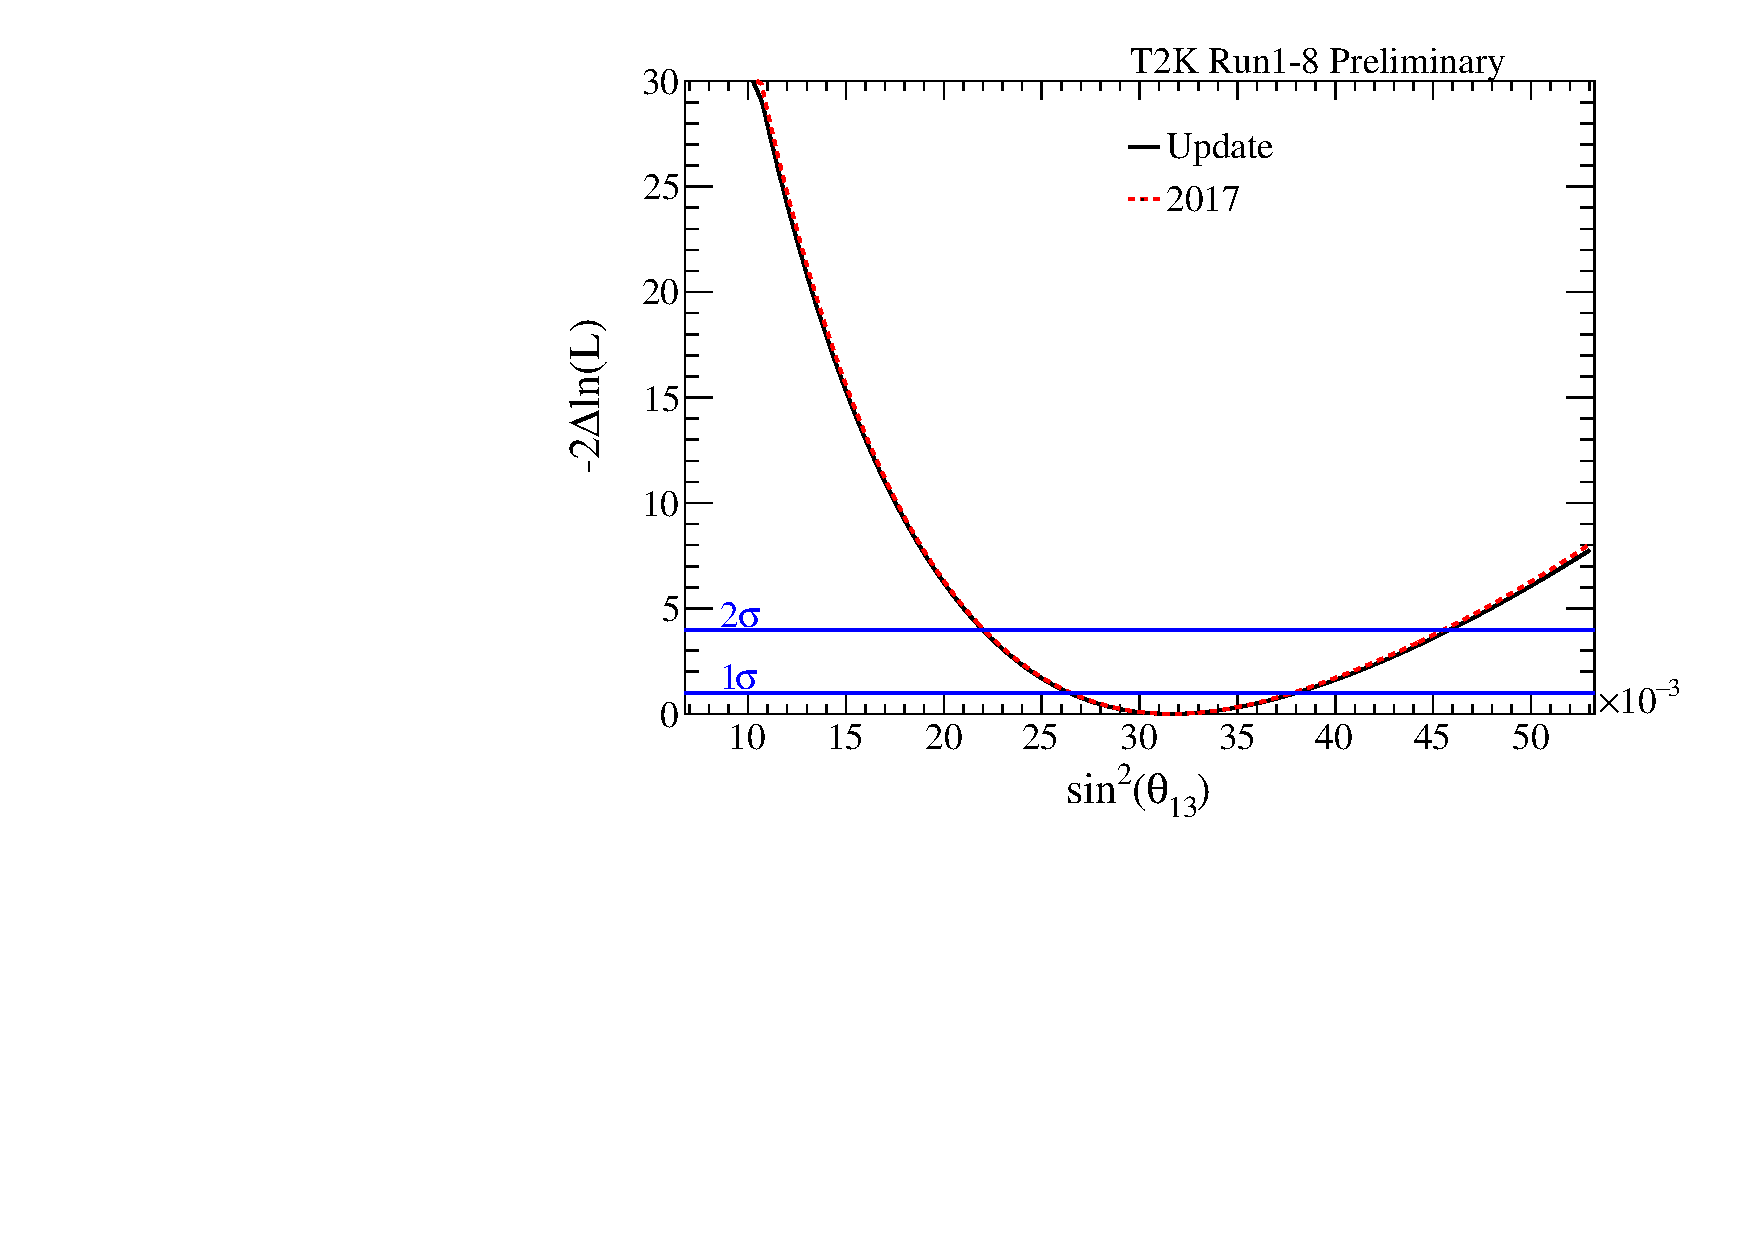
\includegraphics[width=0.9\textwidth]{data/t2k/2017b/comparisons/mixing13_data_t2k_ih}
		\caption{\ssqthonethree IH}
	\end{subfigure}
	\caption {
		The expected $\Delta\chi^2$ distribution as a function of \ssqthonethree without reactor constraint. The mass hierarchy is minimized, with normal and inverted hierarchy $\Delta\chi^2$ distributions shifted to the same global best-fit $\chi^2$ value, which is taken to be the minimum between normal and inverted hierarchy. All 5 samples were used to produce these fits.
	}
	\label{fig:th13_data_compare}
\end{figure*}

\clearpage

\subsubsection{Results for \ssqthtwothree}

The result for \ssqthtwothree with reactor constraint is shown in fig.~\ref{fig:th23_data_compare}.

\begin{figure*}[htb]
	\center
	\begin{subfigure}[b]{0.49\textwidth}
		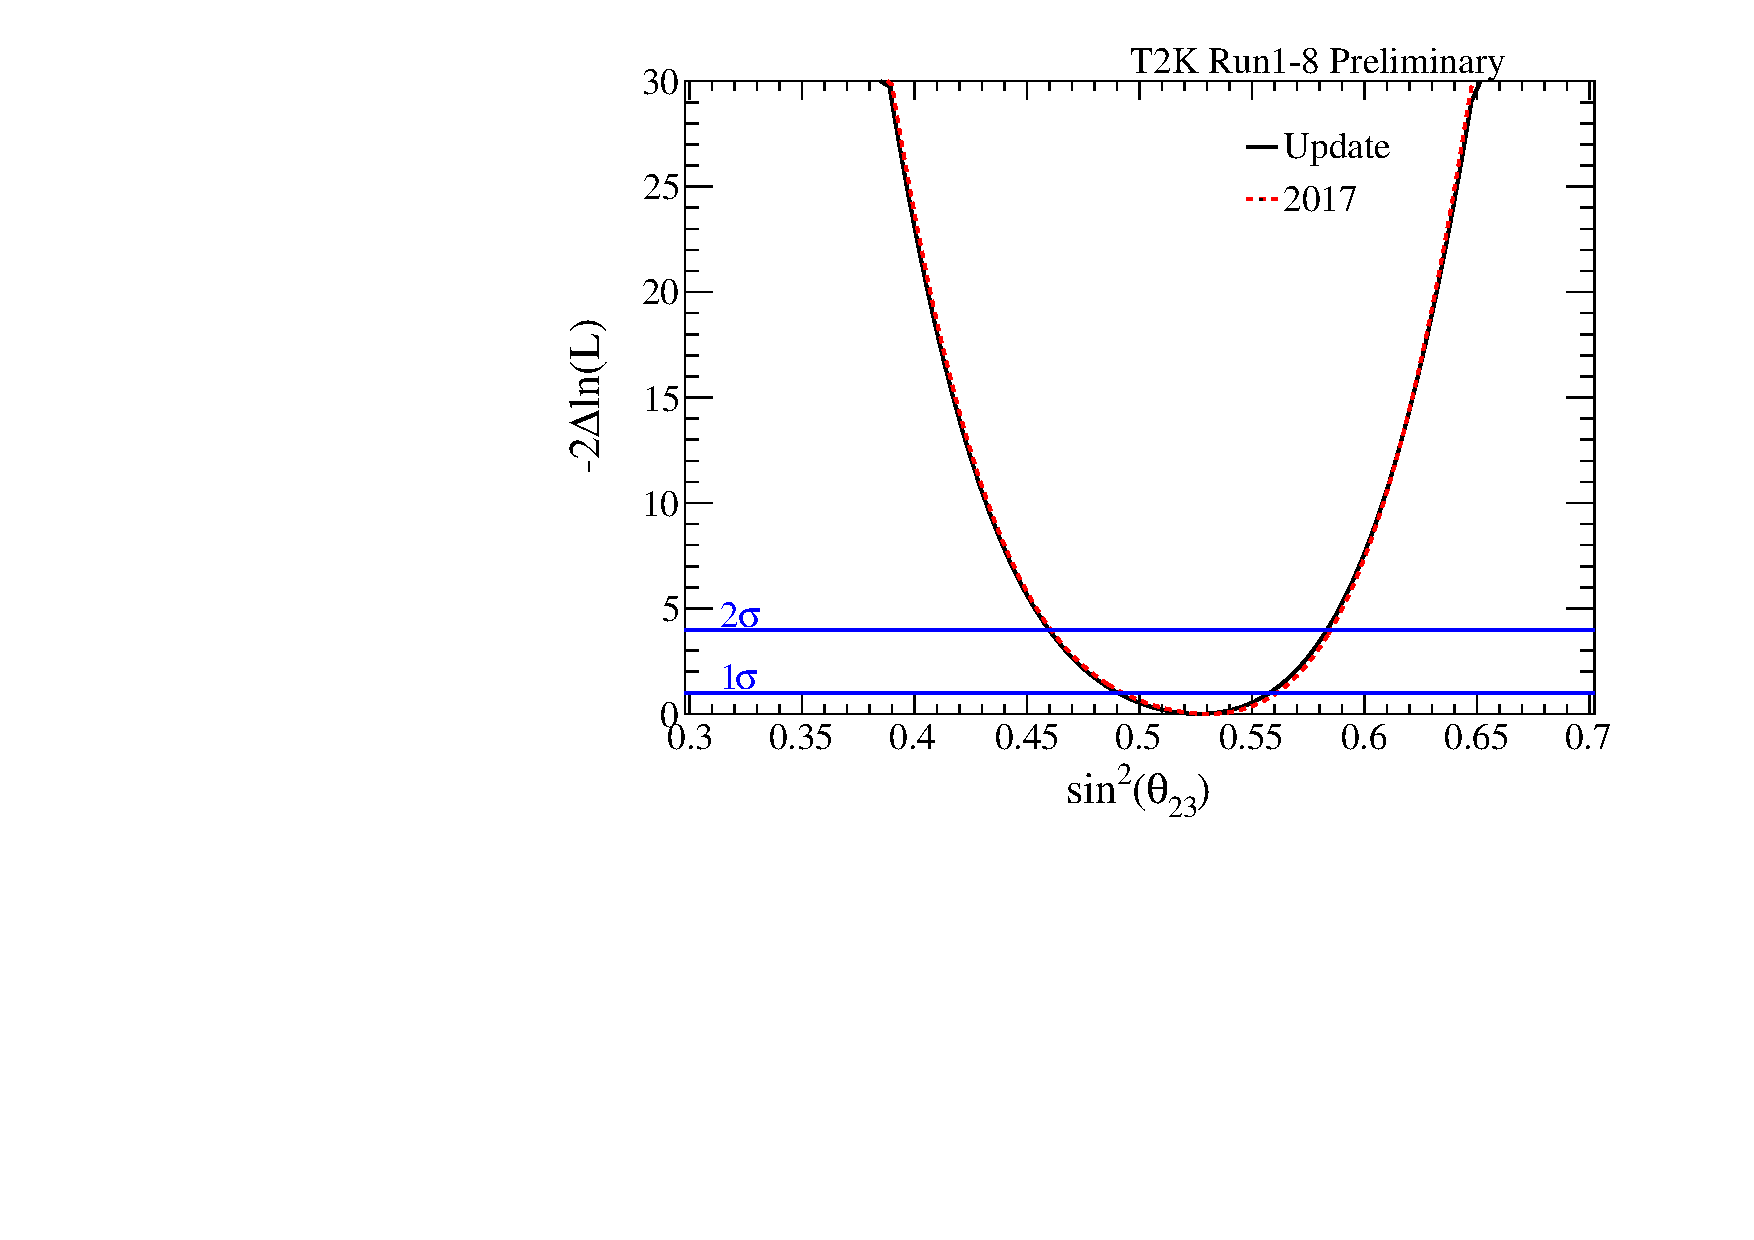
\includegraphics[width=0.9\textwidth]{data/reactor/2017b/comparisons/mixing23_data_reactor_nh}
		\caption{\ssqthtwothree NH}
	\end{subfigure}
	\begin{subfigure}[b]{0.49\textwidth}
		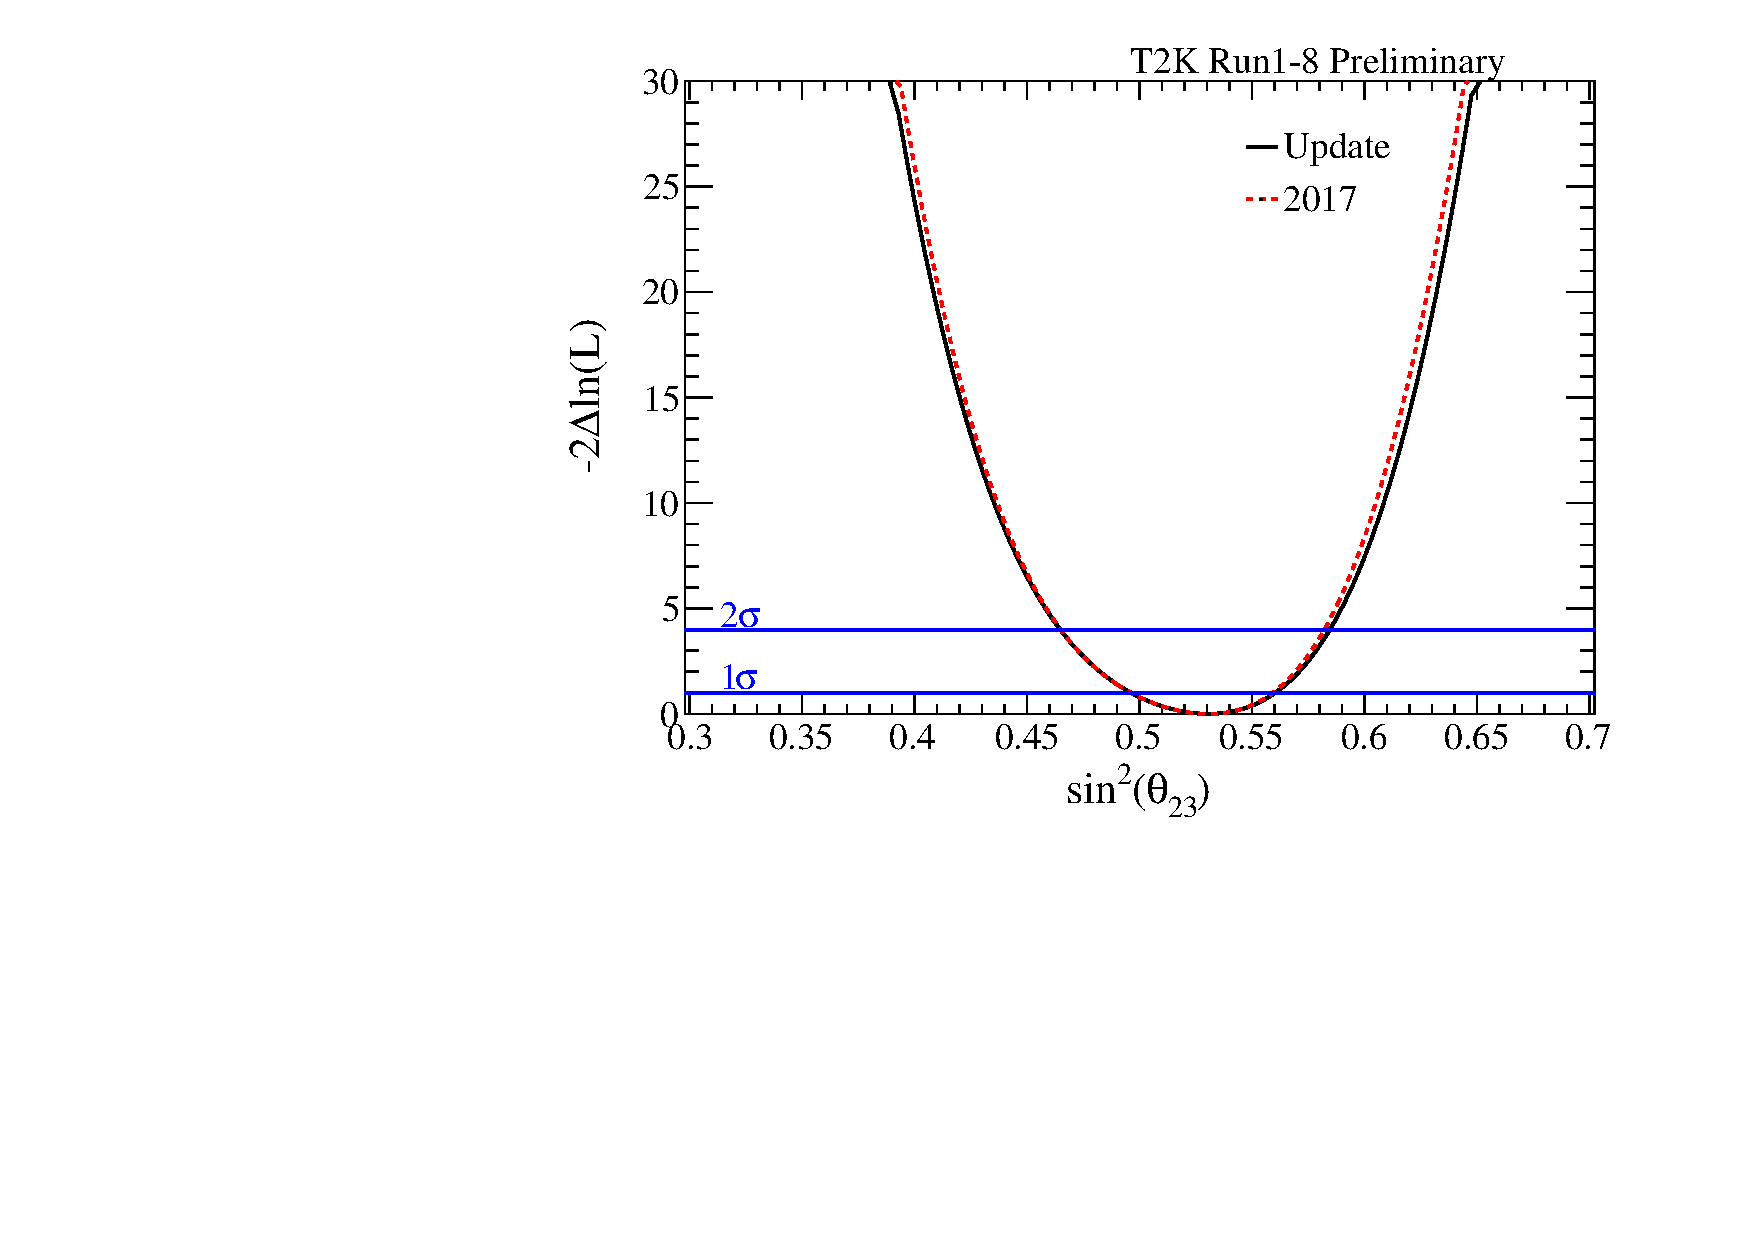
\includegraphics[width=0.9\textwidth]{data/reactor/2017b/comparisons/mixing23_data_reactor_ih}
		\caption{\ssqthtwothree IH}
	\end{subfigure}
	\caption {
		The expected $\Delta\chi^2$ distribution as a function of \ssqthtwothree with reactor constraint. The mass hierarchy is minimized, with normal and inverted hierarchy $\Delta\chi^2$ distributions shifted to the same global best-fit $\chi^2$ value, which is taken to be the minimum between normal and inverted hierarchy. All 5 samples were used to produce these fits.
	}
	\label{fig:th23_data_compare}
\end{figure*}

\subsubsection{Results for \dmsq}

The result for \dmsq with reactor constraint is shown in fig.~\ref{fig:dmsq23_data_compare}.

\begin{figure*}[htb]
	\center
	\begin{subfigure}[b]{0.49\textwidth}
		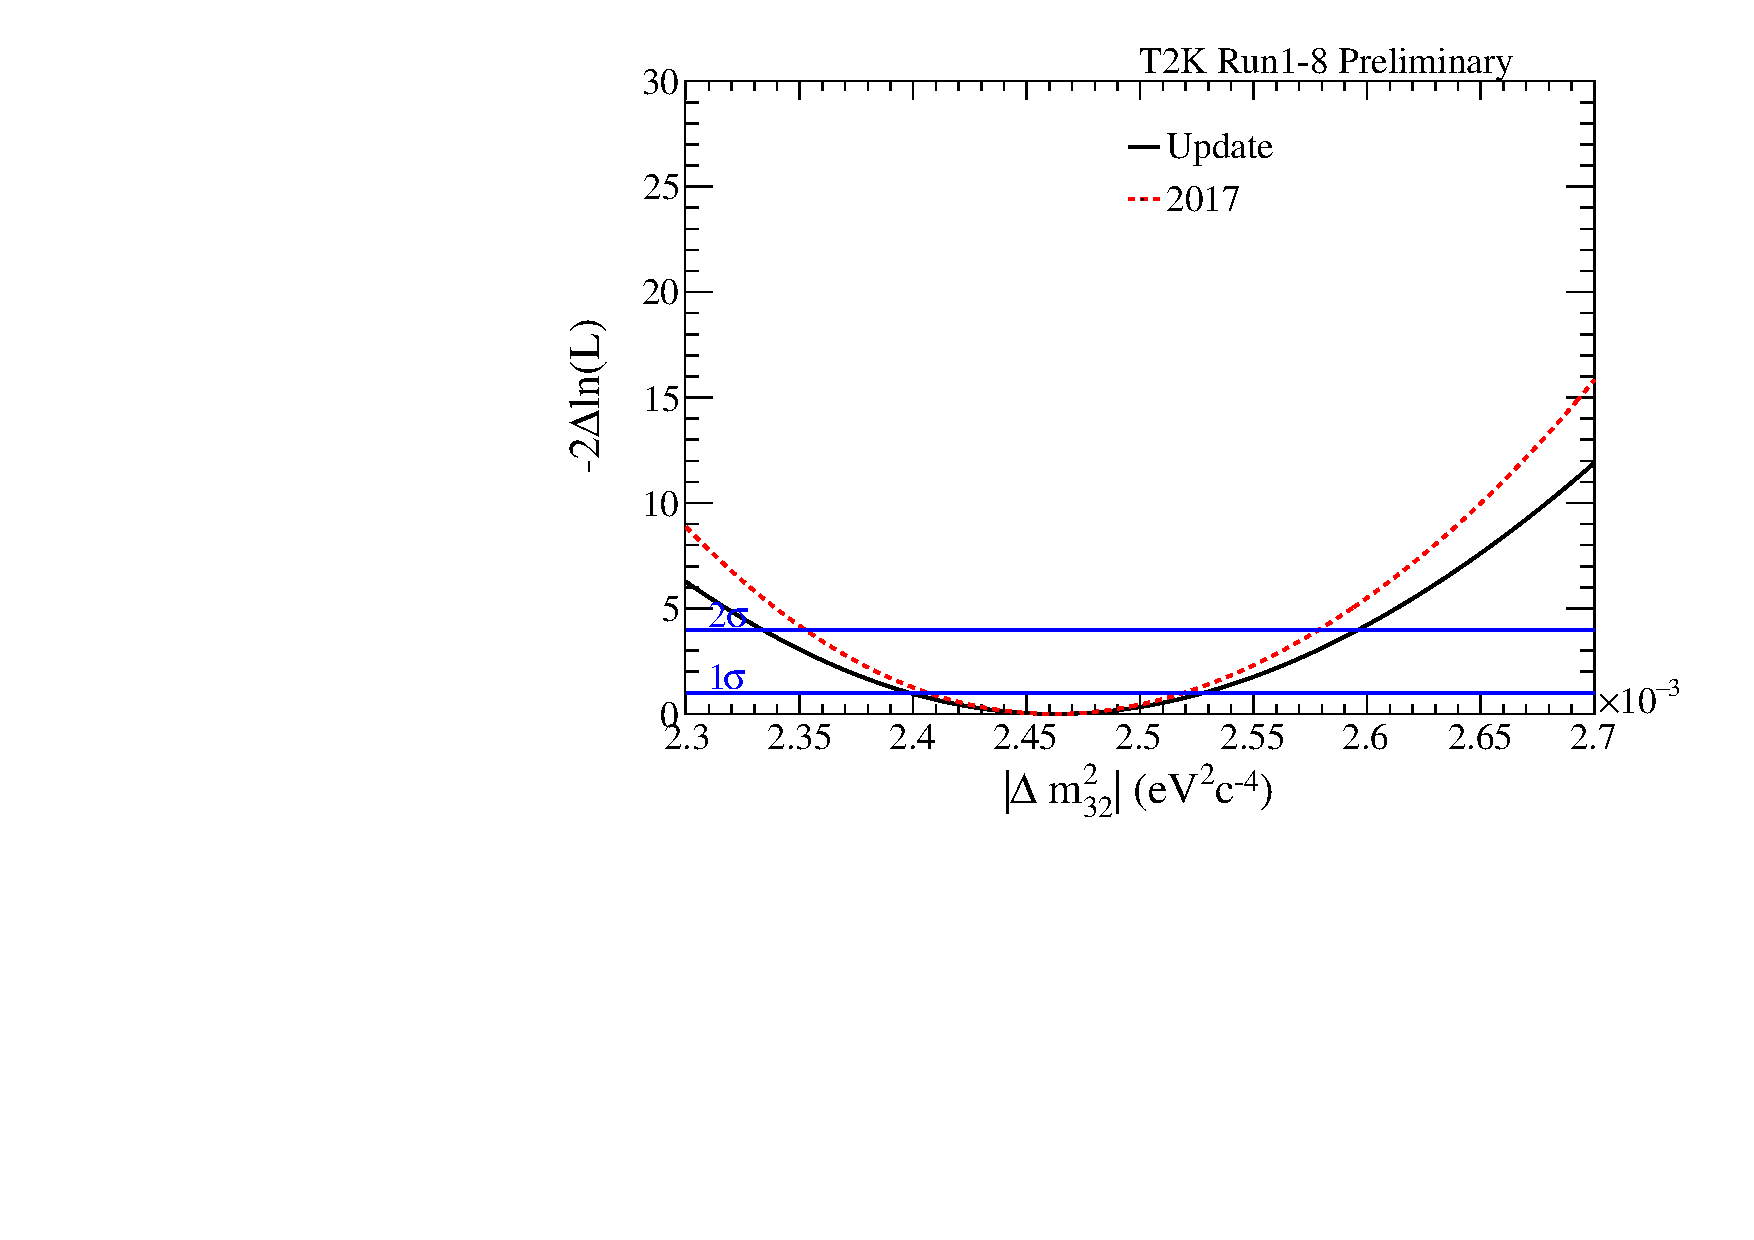
\includegraphics[width=0.9\textwidth]{data/reactor/2017b/comparisons/dmsq23_data_reactor_nh}
		\caption{\dmsq NH}
	\end{subfigure}
	\begin{subfigure}[b]{0.49\textwidth}
		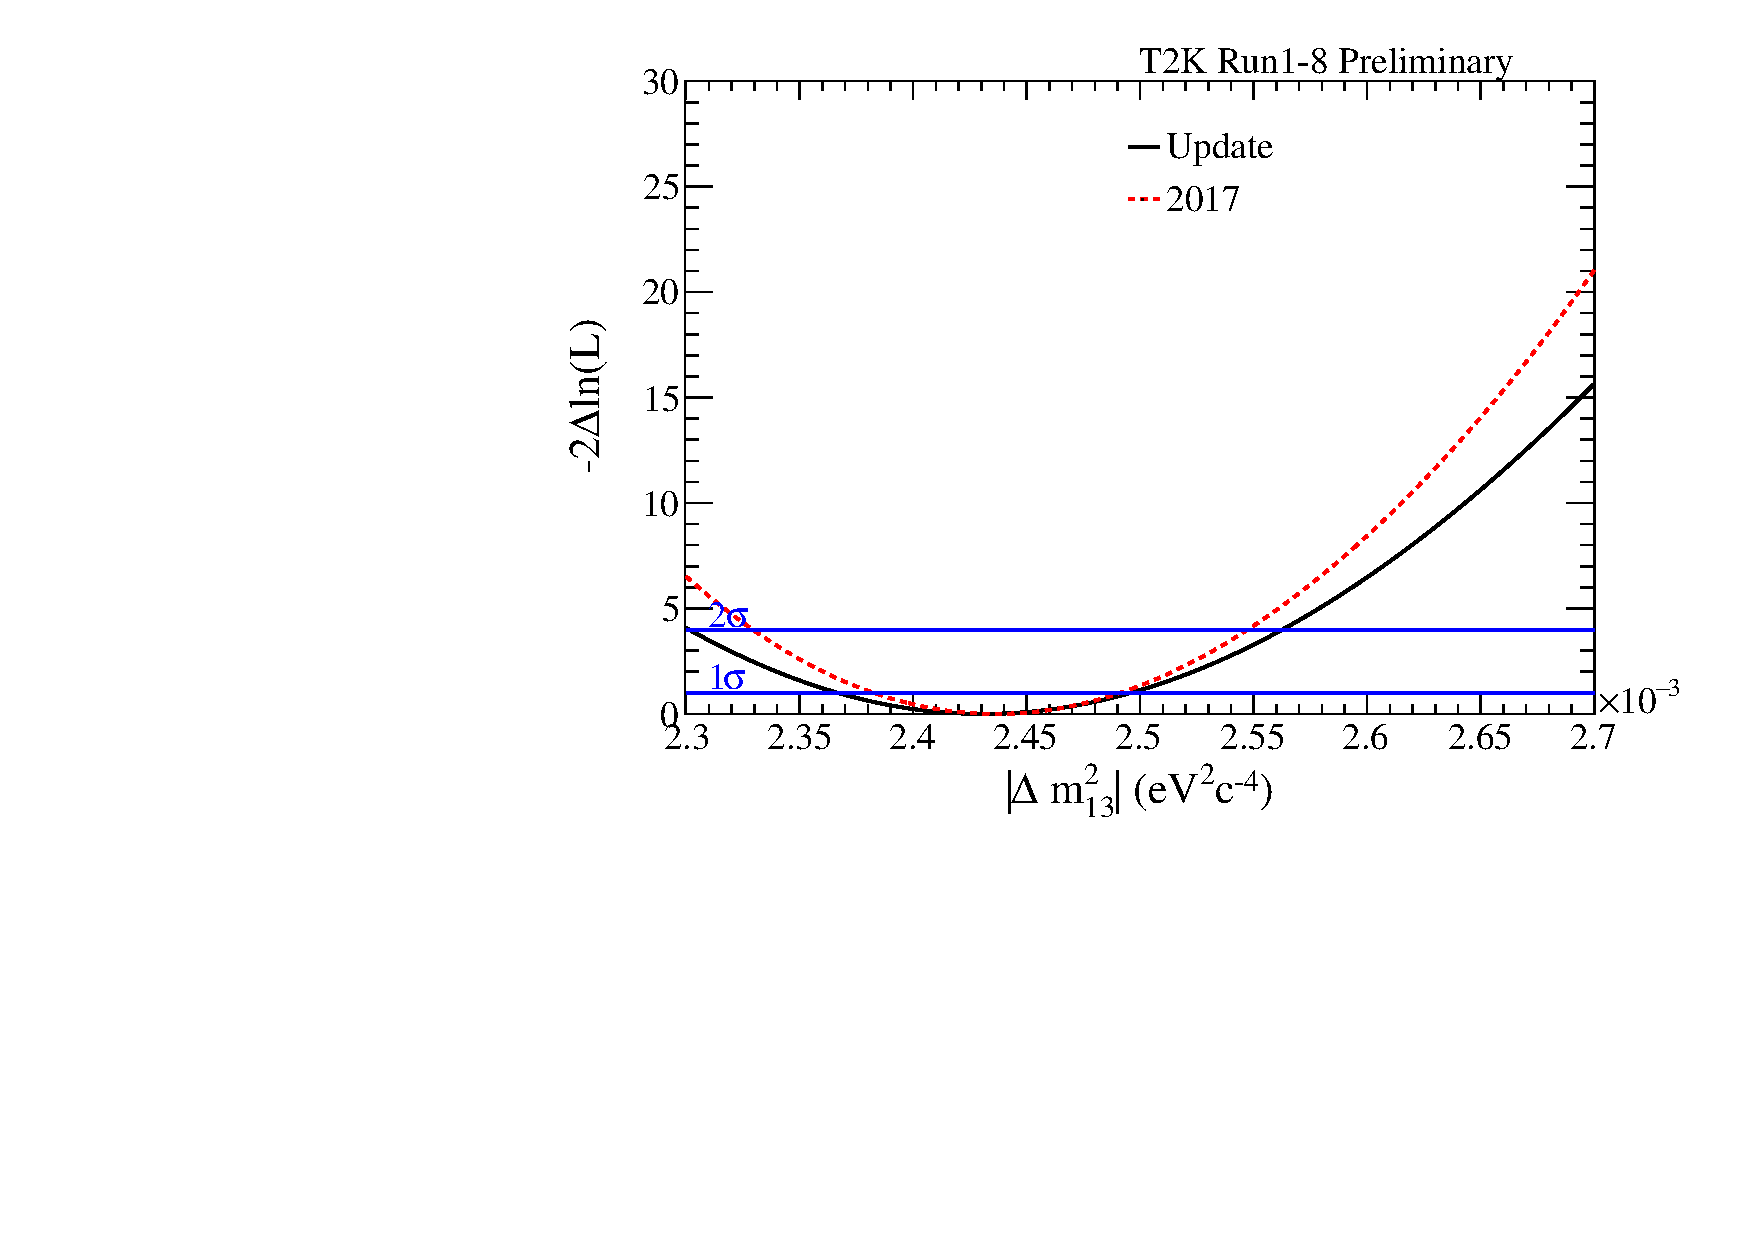
\includegraphics[width=0.9\textwidth]{data/reactor/2017b/comparisons/dmsq23_data_reactor_ih}
		\caption{\dmsq IH}
	\end{subfigure}
	\caption {
		The expected $\Delta\chi^2$ distribution as a function of \dmsq with reactor constraint. The mass hierarchy is minimized, with normal and inverted hierarchy $\Delta\chi^2$ distributions shifted to the same global best-fit $\chi^2$ value, which is taken to be the minimum between normal and inverted hierarchy. All 5 samples were used to produce these fits.
	}
	\label{fig:dmsq23_data_compare}
\end{figure*}

\subsection {Discussion of the \RunPeriod data fit results}
\label{sec:results:discussion_2017b}

It can be seen from section \cref{sec:results:comparison} that the majority of fits show little change between the 2017 and updated analyses for fits of \ssqthonethree, \ssqthtwothree and \deltacp. The best-fit values show changes of no more than a single bin in the fit parameter; this being most evident in the normal hierarchy \appearance fit, where the binning is coarser. The contours for the \appearance fit are almost identical. A moderate inflation of the T2K-only \ssqthonethree contour in normal hierarchy can be seen. \color{blue}A possible explanation of the asymmetry in the inflation of this contour is that as the value of \ssqthonethree increases a larger combination of values of other oscillation parameters can produce equivalent spectra; the addition of the Eb parameter then provides additional freedom in this respect and thereby weakens the fit in this region. The effect diminishes for smaller values of \ssqthonethree as there is less of an appearance signal for Eb to act upon\color{black}. Modest changes in the \deltacp contours are evident, with slightly less extreme values of $\Delta\chi^2$ around the peak near $\delta_{CP}=\pi/2$, but this does not alter the rejection of CP conservation at $2\sigma$, as demonstrated in \cref{sec:fc_significance:intervals_2017b}.

Differences are evident in the fits of the atmospheric parameters, particularly \dmsq. The addition of the Eb parameter and \dmsq smearing has inflated the contours, most notably in the \dmsq parameter, as expected. The best-fit point is little changed in normal hierarchy (again being most evident in the coarser-binned 2D fit), and a small shift in \dmsq is observed in both 2D and 1D fits in inverted hierarchy. The 1D fits of \ssqthtwothree show slight inflation of the contours, with the inflation clearly evident in the 1D fits of \dmsq.

\clearpage

%%% Local Variables:
%%% mode: latex
%%% TeX-master: "../TN327"
%%% End:
